% ============================================================================================
% European and American option pricing: binomial trees, Monte Carlo and the variational PDE
% Structure, equations, tables and figures live in this file; every prose paragraph lives in
% paras/Pxx.tex (one file per paragraph, draft sentences to be rewritten) and is pulled in with \input.
% Every number in the prose is a macro defined in macros.tex, which the notebook regenerates.
% Build:  pdflatex main && bibtex main && pdflatex main && pdflatex main
% ============================================================================================
\documentclass[12pt]{amsart}
\usepackage{amsthm,amssymb,amsmath}
\usepackage{graphicx}
\usepackage{booktabs}
\usepackage{listings}
\usepackage{multicol}
\usepackage{placeins}
\usepackage{natbib}
\usepackage{xcolor}
\usepackage[colorlinks=true,linkcolor=blue!50!black,citecolor=blue!50!black,urlcolor=blue!50!black]{hyperref}

\textwidth 175mm
\oddsidemargin -5mm
\evensidemargin -5mm
\textheight 230mm
\topmargin -10mm

\graphicspath{{figures/}}
% AUTO-GENERATED by notebooks/option_pricing.ipynb: do not edit by hand
\newcommand{\AmBearly}{7.4}
\newcommand{\AmBhalf}{7.87}
\newcommand{\AmV}{0.7110}
\newcommand{\AmVegaTree}{3.90}
\newcommand{\AmVeight}{0.7109}
\newcommand{\AmVzero}{0.7109}
\newcommand{\BAWSc}{7.55}
\newcommand{\BAWV}{0.7100}
\newcommand{\BAWerr}{\ensuremath{-}0.0011}
\newcommand{\BSdOne}{0.2655}
\newcommand{\BSdTwo}{\ensuremath{-}0.1118}
\newcommand{\BSdelta}{0.6047}
\newcommand{\BSgamma}{0.00427}
\newcommand{\BSprice}{38.7493}
\newcommand{\BSput}{31.9207}
\newcommand{\BSrho}{105.71}
\newcommand{\BSrhoPct}{1.057}
\newcommand{\BStheta}{\ensuremath{-}20.42}
\newcommand{\BSthetaDay}{\ensuremath{-}0.056}
\newcommand{\BSvega}{92.01}
\newcommand{\BSvegaPct}{0.920}
\newcommand{\BermFifty}{0.7105}
\newcommand{\BhalfHigh}{6.68}
\newcommand{\BhalfLow}{9.06}
\newcommand{\BhalfMid}{7.86}
\newcommand{\BhalfRhigh}{8.20}
\newcommand{\BoundGap}{0.10}
\newcommand{\CRRerrHundredOdd}{\ensuremath{8.4\times10^{-2}}}
\newcommand{\CRRhundredErr}{0.0882}
\newcommand{\CRRtenk}{38.7484}
\newcommand{\CRRtenkErr}{0.0009}
\newcommand{\CRRthousandErr}{0.0088}
\newcommand{\DeltaPathOneEnd}{\ensuremath{-}0.99}
\newcommand{\DeltaRangeHi}{\ensuremath{-}0.41}
\newcommand{\DeltaRangeLo}{\ensuremath{-}0.48}
\newcommand{\DeltaStart}{\ensuremath{-}0.44}
\newcommand{\DeskBawErr}{0.0011}
\newcommand{\DeskBawMs}{1}
\newcommand{\DeskCrrClassMs}{12}
\newcommand{\DeskCrrThousandMs}{3.4}
\newcommand{\DeskCrrVecErr}{\ensuremath{-}0.035}
\newcommand{\DeskCrrVecMs}{0.6}
\newcommand{\DeskLrErr}{0.0002}
\newcommand{\DeskLrMs}{0.2}
\newcommand{\DeskLsmErr}{0.0016}
\newcommand{\DeskLsmMs}{1402}
\newcommand{\DeskLsmSE}{0.0019}
\newcommand{\DeskMcCvErr}{0.068}
\newcommand{\DeskMcCvSE}{0.082}
\newcommand{\DeskMcEulerMs}{398.1}
\newcommand{\DeskMcPlainErr}{0.209}
\newcommand{\DeskMcPlainMs}{3.5}
\newcommand{\DeskMcPlainSE}{0.215}
\newcommand{\DeskPdeCoarseErr}{0.00008}
\newcommand{\DeskPdeCoarseMs}{132}
\newcommand{\DeskPdeFineErr}{0.00001}
\newcommand{\DeskPdeFineMs}{1361}
\newcommand{\DeskPutClassMs}{24}
\newcommand{\DeskPutRefMs}{533}
\newcommand{\DeskPutTreeErr}{0.00007}
\newcommand{\DeskPutTreeMs}{51}
\newcommand{\DeskPutVecMs}{15}
\newcommand{\DeskSmoothErr}{0.0000}
\newcommand{\DeskSmoothMs}{2.5}
\newcommand{\DeskSobolErr}{0.0013}
\newcommand{\DeskSobolMs}{2.6}
\newcommand{\DivPremSix}{0.229}
\newcommand{\EEPatm}{0.0175}
\newcommand{\EEPatmPct}{2.5}
\newcommand{\EEPmaxPct}{13}
\newcommand{\EMstrongSlope}{\ensuremath{-}0.49}
\newcommand{\EMweakSlope}{\ensuremath{-}0.96}
\newcommand{\HedgeSDdaily}{1.91}
\newcommand{\HedgeSDdailyPct}{4.9}
\newcommand{\HedgeSDfour}{14.19}
\newcommand{\HedgeSDweekly}{4.15}
\newcommand{\HedgeSDweeklyPct}{10.7}
\newcommand{\HedgeSlope}{\ensuremath{-}0.49}
\newcommand{\IVcrrHundred}{\ensuremath{-}0.10}
\newcommand{\IVmcHi}{37.90}
\newcommand{\IVmcLo}{37.49}
\newcommand{\KSconst}{0.399}
\newcommand{\LRerrHundred}{\ensuremath{1.7\times10^{-4}}}
\newcommand{\LRerrThousand}{\ensuremath{1.7\times10^{-6}}}
\newcommand{\LSMfifty}{0.7095}
\newcommand{\LSMfiftySE}{0.0018}
\newcommand{\LatBcoarse}{5.25}
\newcommand{\LatBfine}{5.09}
\newcommand{\LatVgap}{0.00085}
\newcommand{\LatVgapCoarse}{0.00303}
\newcommand{\LongBhundred}{5.20}
\newcommand{\LongBthousand}{5.18}
\newcommand{\LongDecay}{0.040}
\newcommand{\LongFloor}{0.0020}
\newcommand{\LongGapThousand}{\ensuremath{2.0\times10^{-3}}}
\newcommand{\LongVthousand}{2.4980}
\newcommand{\MCbest}{38.7236}
\newcommand{\MCbestErr}{0.0257}
\newcommand{\MCbestSE}{0.096}
\newcommand{\MCcoverage}{95.2}
\newcommand{\MCdeltaPW}{0.6048}
\newcommand{\MCgammaBumpSE}{0.00003}
\newcommand{\MCgammaLR}{0.00428}
\newcommand{\MCgammaLRSE}{0.00001}
\newcommand{\MapPaths}{100\,000}
\newcommand{\MapPnLmismatch}{\ensuremath{+}0.45}
\newcommand{\MapRegretHighLow}{0.017}
\newcommand{\MapRegretLowHigh}{0.326}
\newcommand{\MapRegretMax}{0.326}
\newcommand{\MapSE}{0.0034}
\newcommand{\MaxGapTen}{0.238}
\newcommand{\MaxGapTwoHundred}{0.049}
\newcommand{\MisHighLoss}{0.036}
\newcommand{\MisHighPnL}{\ensuremath{+}0.35}
\newcommand{\MisHighTau}{0.766}
\newcommand{\MisHighTauOpt}{0.883}
\newcommand{\MisLowLoss}{0.016}
\newcommand{\MisLowPnL}{\ensuremath{-}0.41}
\newcommand{\MisLowTau}{0.977}
\newcommand{\MisLowTauOpt}{0.854}
\newcommand{\NvdaBhalf}{147.8}
\newcommand{\NvdaBhalfPct}{61.9}
\newcommand{\NvdaPutAm}{32.5674}
\newcommand{\NvdaPutDelta}{\ensuremath{-}0.407}
\newcommand{\NvdaPutDeltaEu}{\ensuremath{-}0.395}
\newcommand{\NvdaPutEEP}{0.6467}
\newcommand{\NvdaPutEEPpct}{2.03}
\newcommand{\NvdaPutEu}{31.9207}
\newcommand{\NvdaPutIV}{38.43}
\newcommand{\NvdaPutIVup}{0.70}
\newcommand{\NvdaR}{2.9}
\newcommand{\NvdaS}{238.90}
\newcommand{\NvdaSigma}{37.73}
\newcommand{\ParityHi}{0.1980}
\newcommand{\ParityLo}{0.0000}
\newcommand{\ParityMid}{0.1805}
\newcommand{\ParityNvda}{\ensuremath{3\times10^{-14}}}
\newcommand{\PathOneTau}{0.48}
\newcommand{\PdeEuErr}{\ensuremath{9\times10^{-6}}}
\newcommand{\PdeTreeDiff}{\ensuremath{9.5\times10^{-6}}}
\newcommand{\PdeV}{0.71107}
\newcommand{\PerpBeta}{1}
\newcommand{\PerpResidual}{\ensuremath{8\times10^{-9}}}
\newcommand{\PerpSstar}{5}
\newcommand{\PerpV}{2.5}
\newcommand{\PnLPes}{1.54}
\newcommand{\PnLPmean}{\ensuremath{-}0.094}
\newcommand{\PnLPmeanTen}{\ensuremath{-}0.246}
\newcommand{\PnLPpex}{0.46}
\newcommand{\PnLPqNinetyNine}{1.63}
\newcommand{\PnLPsd}{0.81}
\newcommand{\PnLPtau}{0.894}
\newcommand{\PnLPtot}{54.4}
\newcommand{\PnLQes}{1.56}
\newcommand{\PnLQmean}{\ensuremath{-}0.0041}
\newcommand{\PnLQqNinetyNine}{1.63}
\newcommand{\PnLQse}{0.0026}
\newcommand{\PnLQtot}{48.8}
\newcommand{\PnLmean}{\ensuremath{-}0.004}
\newcommand{\PnLpex}{0.52}
\newcommand{\PnLsd}{0.83}
\newcommand{\PnLse}{0.008}
\newcommand{\PnLtau}{0.877}
\newcommand{\QVBMtenk}{1.0000}
\newcommand{\RegretSE}{0.007}
\newcommand{\ReplError}{\ensuremath{4\times10^{-15}}}
\newcommand{\SawEven}{\ensuremath{-}8.81}
\newcommand{\SawOdd}{8.54}
\newcommand{\TVBMtenk}{79.8}
\newcommand{\TVtheorytenk}{79.8}
\newcommand{\TreeDelta}{0.6047}
\newcommand{\TreeGamma}{0.00428}
\newcommand{\TreeRichV}{0.71108}
\newcommand{\TreeVega}{91.98}
\newcommand{\TwoStepAm}{0.6527}
\newcommand{\TwoStepDelta}{\ensuremath{-}0.4647}
\newcommand{\TwoStepEu}{0.6034}
\newcommand{\VRM}{262\,144}
\newcommand{\VRanti}{1.8}
\newcommand{\VRcv}{7.7}
\newcommand{\VRsobol}{76727}
\newcommand{\WPcrrMs}{94}
\newcommand{\WPcrrN}{10\,000}
\newcommand{\WPcvSec}{21}
\newcommand{\WPlrMs}{0.10}
\newcommand{\WPlrN}{41}
\newcommand{\WPmcM}{4.6\times10^{9}}
\newcommand{\WPmcSec}{162}
\newcommand{\WPsmMs}{2}
\newcommand{\WPsmN}{201}
\newcommand{\WPsobolM}{131\,072}
\newcommand{\WPtol}{0.001}
\newcommand{\WrongMuPrice}{49.96}
\newcommand{\WrongVolLoss}{\ensuremath{-}15.78}
\newcommand{\WrongVolTheory}{\ensuremath{-}15.72}
                      % numbers generated by notebooks/option_pricing.ipynb

\newtheorem*{remark}{Remark}
\renewcommand{\topfraction}{0.9}\renewcommand{\bottomfraction}{0.9}\renewcommand{\textfraction}{0.08}\renewcommand{\floatpagefraction}{0.75}
\lstset{basicstyle=\ttfamily\fontsize{5}{6}\selectfont,breaklines=true,columns=fullflexible,keepspaces=true,language=Python,
        commentstyle=\itshape,showstringspaces=false}

\title[Option pricing: trees, Monte Carlo, PDE]{European and American Option Pricing:\\ Binomial Trees, Monte Carlo and the Variational PDE}
\author{Bolong Tang}

\begin{document}

\begin{abstract}
% P00 | Abstract | Abstract
% guide: dev_notes/paragraph_guides/P00_abstract.txt
We compare discrete-time and continuous-time models for pricing and hedging options on two problems: a one-year at-the-money European call on NVIDIA and an American put.
A scaled symmetric random walk converges to Brownian motion, with a Kolmogorov distance at the terminal time that falls like $N^{-1/2}$ with the exact constant \KSconst.
Path functionals such as the running maximum converge at the same slow rate, which is why discretely monitored barriers need a correction.
The CRR tree reaches the Black--Scholes price of \$\BSprice\ to within \$\CRRtenkErr\ at $N=10{,}000$ steps, whereas the Euler--Maruyama Monte Carlo price has a standard error of \$\MCbestSE\ at $5\cdot10^5$ paths.
A Leisen--Reimer tree with only 101 steps is accurate to \$\DeskLrErr, and a control variate reduces the Monte Carlo variance by a factor of \VRcv.
For the American put, a CRR tree, a finite-difference solver for the variational inequality and least-squares Monte Carlo agree on a value of about \TreeRichV\ for the baseline contract, and the early-exercise premium is \EEPatmPct\% of the European put at the money.
On the NVIDIA inputs the American put is worth \$\NvdaPutAm, \NvdaPutEEPpct\% more than the European put.
Daily delta hedging of the call leaves a hedging error with a standard deviation of \HedgeSDdailyPct\% of the premium, and a wrong volatility distorts the American exercise rule asymmetrically: exercising too early costs about twenty times as much as exercising too late in our worst cases.

\end{abstract}

\maketitle

% ======================================================================================== 1
\section{Introduction}
% P01 | 1 Introduction | Motivation: why numerical option pricing
% guide: dev_notes/paragraph_guides/P01_motivation_why_numerical_option_pricing.txt
Option prices are needed continuously, for thousands of contracts at a time, both to quote them and to measure the risk of a book.
A closed-form price exists only for the simplest contracts, so in practice trees, Monte Carlo simulation and PDE solvers do most of the work, and each of them trades accuracy against computing time.
These methods come from two modelling languages: a discrete-time language, in which the stock follows a random walk on a lattice, and a continuous-time language, in which it follows a geometric Brownian motion.
The two languages describe the same market in the limit of small time steps, so the useful question is not whether they agree but how quickly, and at what computational price.
We study two contracts that stress the methods in different ways.
The European call on NVIDIA has a closed-form Black--Scholes price and is therefore a clean benchmark, whereas the American put has no closed form because its holder may exercise at any time and the optimal exercise boundary has to be found together with the price.
The question we answer is a practical one: which method should be used for which job, given measured errors and measured run times?


% P02 | 1 Introduction | Roadmap of the three parts
% guide: dev_notes/paragraph_guides/P02_roadmap_of_the_three_parts.txt
Section~\ref{sec:A} shows that a scaled symmetric random walk converges to Brownian motion and measures the convergence in three ways: quadratic and total variation, an exact Kolmogorov distance at the terminal time, and the law of the running maximum.
This is the bridge between the discrete and the continuous language, because the binomial tree is a random walk with drift.
Section~\ref{sec:B} prices a one-year at-the-money call on NVIDIA with the Cox--Ross--Rubinstein (CRR) tree and with Monte Carlo simulation of geometric Brownian motion, and benchmarks both against Black--Scholes.
It then asks what a practitioner would ask next: how to make each method more accurate, how to compute sensitivities, how to read the price as an implied volatility, and how well the option can be hedged in discrete time.
Section~\ref{sec:C} turns to the American put: the optimal stopping problem and its variational PDE, the closed-form perpetual put, the CRR tree with its exercise boundary and hedge, and independent checks by a finite-difference solver, least-squares Monte Carlo and a quasi-analytic approximation.
It closes with the early-exercise premium, dividends, an American put on the NVIDIA inputs, and the profit and loss of the buyer under the pricing measure and under the real-world measure.
Section~\ref{sec:compare} compares every method on accuracy and run time, and Section~\ref{sec:concl} states the conclusions and their limits.


% P03 | 1 Introduction | How the work is organised and reproduced
% guide: dev_notes/paragraph_guides/P03_how_the_work_is_organised_and_reproduced.txt
The classes that were written by hand (\texttt{BrownianMotion}, \texttt{symmetric\_random\_walk}, \texttt{CRRBinomialModel}, \texttt{CRRTree} and the two GBM simulators) are used exactly as written.
Every extension is a subclass or a new function placed after them and marked \texttt{[EXT]} in the notebook, so each added result can be traced back to the original code it builds on.
A single notebook produces every figure, table and number in this report, all random numbers are seeded, and the numbers quoted in the text are read from a file generated by the notebook.
A complete run takes about ten minutes on one core.
The scope is deliberately narrow: constant volatility, a constant interest rate and no dividends, except in the one section where a dividend yield is introduced on purpose.
These are the assumptions under which every method in the report can be compared against an exact or near-exact answer.
Full derivations are collected in Appendix~\ref{app:derivations} and the code listing is in Appendix~\ref{app:code}.


% ======================================================================================== 2
\section{Setting and notation}\label{sec:setting}
% P04 | 2 Setting and notation | The market model and risk-neutral pricing
% guide: dev_notes/paragraph_guides/P04_the_market_model_and_risk_neutral_pricing.txt
The market has a bond $B_t=e^{rt}$ and a stock whose price follows, under the real-world measure $\mathbb P$,
\begin{equation}\label{eq:gbm}
 dS_t=\mu S_t\,dt+\sigma S_t\,dW_t,
\end{equation}
where $W$ is a Brownian motion, $\mu$ is the real-world drift and $\sigma$ the volatility.
Under the risk-neutral measure $\mathbb Q$ the drift $\mu$ is replaced by $r$, so that $e^{-rt}S_t$ is a martingale, and the arbitrage-free price at time $0$ of a European claim paying $h(S_T)$ is $e^{-rT}\mathbb E^{\mathbb Q}[h(S_T)]$.
The drift $\mu$ therefore plays no role in pricing; it matters only when we simulate profit and loss under $\mathbb P$ in Section~\ref{sec:C}.
We assume a constant volatility and interest rate, no dividends, no transaction costs and trading in continuous time, which are the textbook assumptions and are violated in real markets in ways that Section~\ref{sec:concl} lists.
Dividends are introduced in Section~\ref{sec:div} and discrete trading in Section~\ref{sec:hedge}.
With one stock driven by one Brownian motion and one bond the market is complete, so $\mathbb Q$ is unique and every claim is replicable by a self-financing portfolio.
This is what makes the price of an option the cost of its hedge, and it is the principle behind the hedging experiments of Sections~\ref{sec:hedge} and~\ref{sec:replication}.


% P05 | 2 Setting and notation | Data and parameters
% guide: dev_notes/paragraph_guides/P05_data_and_parameters.txt
The European problem uses the NVIDIA (NVDA) closing price of \$\NvdaS\ on 2026-10-05, a strike $K=S_0$ (at the money) and a maturity of one year, which is 252 trading days.
Time is measured in trading years, so a tree step of one day is $\Delta t=1/252$.
The volatility is the standard deviation of the last 250 daily log returns multiplied by $\sqrt{252}$, which gives $\sigma=\NvdaSigma\%$.
Using a historical volatility assumes that the next year looks like the last one; an implied volatility from market quotes would replace it in practice.
The risk-free rate is the Bank of Canada one-year Treasury-bill yield, $r=\NvdaR\%$, chosen to match the one-year maturity.
A Canadian rate is not the natural choice for a US-dollar asset, but the call is not very sensitive to it: its rho is about \BSrhoPct\ dollars per percentage point of the rate (Section~\ref{sec:B-greeks}).
The American put uses a deliberately simple baseline, $S_0=K=10$, $\sigma=20\%$, $r=2\%$, $T=1$ and a real-world drift $\mu=5\%$, for which the perpetual limit is known exactly.
Because the exercise boundary scaled by the strike depends only on $\sigma$, $r$ and the time to maturity, results for this baseline carry over to any strike; Table~\ref{tbl:params} lists both parameter sets.


\begin{table}[h!]
\centering
\begin{tabular}{lcc}
\toprule
 & European call (Part B) & American put (Part C)\\
\midrule
Underlying & NVDA, close of 2026-10-05 & generic, unit-free\\
Spot $S_0$ and strike $K$ & $\NvdaS$ and $K=S_0$ & $10$ and $K=S_0$\\
Volatility $\sigma$ & $\NvdaSigma\%$ (historical, 252 days) & $20\%$ (varied: $10\%$, $30\%$)\\
Interest rate $r$ & $\NvdaR\%$ (Bank of Canada, 1 year) & $2\%$ (varied: $0\%$, $4\%$)\\
Maturity $T$ & 1 year (252 trading days) & 1 year (varied up to $\infty$)\\
Real-world drift $\mu$ & $10\%$ (hedging experiments only) & $5\%$ (profit-and-loss under $\mathbb P$)\\
Dividend yield $q$ & $0$ & $0$ (varied in Section~\ref{sec:div})\\
\bottomrule
\end{tabular}
\caption{Parameters of the two benchmark problems.\label{tbl:params}}
\end{table}

% ======================================================================================== 3
\section{Part A: Brownian motion and scaled random walks}\label{sec:A}
% P06 | 3 Part A: Brownian motion and random walks | Brownian motion and the scaled random walk
% guide: dev_notes/paragraph_guides/P06_brownian_motion_and_the_scaled_random_walk.txt
A process $W=\{W_t\}_{t\ge0}$ is a Brownian motion on $(\Omega,\mathcal F,\{\mathcal F_t\},\mathbb P)$ if it is adapted with $W_0=0$, if $W_t-W_s\sim N(0,t-s)$ for $0\le s\le t$, if $W_t-W_s$ is independent of $\mathcal F_s$, and if $t\mapsto W_t(\omega)$ is continuous.
Independence and the Gaussian law of increments fix all finite-dimensional distributions, and continuity of the paths is what separates Brownian motion from other processes with the same increments.
The scaled symmetric random walk replaces the Gaussian increments by coin flips: with $\xi_i=\pm1$ equally likely,
\begin{equation}\label{eq:scaledwalk}
 W^{(N)}_{t_k}=\sqrt{T/N}\sum_{i=1}^{k}\xi_i,\qquad t_k=kT/N,
\end{equation}
so that $\mathbb E\,W^{(N)}_{t_k}=0$ and $\operatorname{Var}W^{(N)}_{t_k}=t_k$ for every $N$.
Mean, variance and independence of increments therefore agree with Brownian motion for every $N$, whereas the lattice support and the non-Gaussian increments do not.
Donsker's theorem states that the whole path $W^{(N)}$ converges in law to $W$ as $N\to\infty$, which is the statement we test numerically.
This matters for pricing because the CRR tree of Section~\ref{sec:B} is exactly such a walk with a drift, so its convergence to geometric Brownian motion is a consequence of the convergence studied here.


% P07 | 3 Part A: Brownian motion and random walks | How the paths were simulated
% guide: dev_notes/paragraph_guides/P07_how_the_paths_were_simulated.txt
The class \texttt{BrownianMotion} builds a path step by step from independent $N(0,\Delta t)$ increments on $[0,1]$, with $N_1=10{,}000$ steps.
Five independent paths are drawn for the figure.
The subclass \texttt{symmetric\_random\_walk} overrides only the step, replacing the Gaussian draw by $\pm\sqrt{\Delta t}$ with probability one half each.
It is run with $N_2\in\{10,50,200,1000\}$ steps on the same time interval.
For the quantitative checks we add vectorised generators that draw 2000 paths per $N$ and compute quadratic and total variation.
The Kolmogorov distance and the law of the running maximum are computed exactly from the binomial distribution, so they carry no sampling error.


% P08 | 3 Part A: Brownian motion and random walks | Result: sample paths
% guide: dev_notes/paragraph_guides/P08_result_sample_paths.txt
Figure~\ref{fig:part1} shows that the walk with $N_2=10$ makes very few turns and looks like a polygon, whereas the walk with $N_2=1000$ is hard to tell from a Brownian path.
Between these two the number of turns and the roughness of the path grow steadily with $N_2$.
The maxima and minima of the walks are comparable for every $N_2$, because the variance at $t=1$ is equal to $1$ whatever the step size.
What changes with $N_2$ is the fine structure of the path, not its overall range.
Neither object has a derivative, so the Brownian paths are not smoother than the walks: it is the walk that becomes Brownian as $N_2$ grows.
This is the point of Donsker's theorem.
A picture is suggestive but not a measurement, so the next three paragraphs quantify the convergence.


\begin{figure}[h!]
\centering
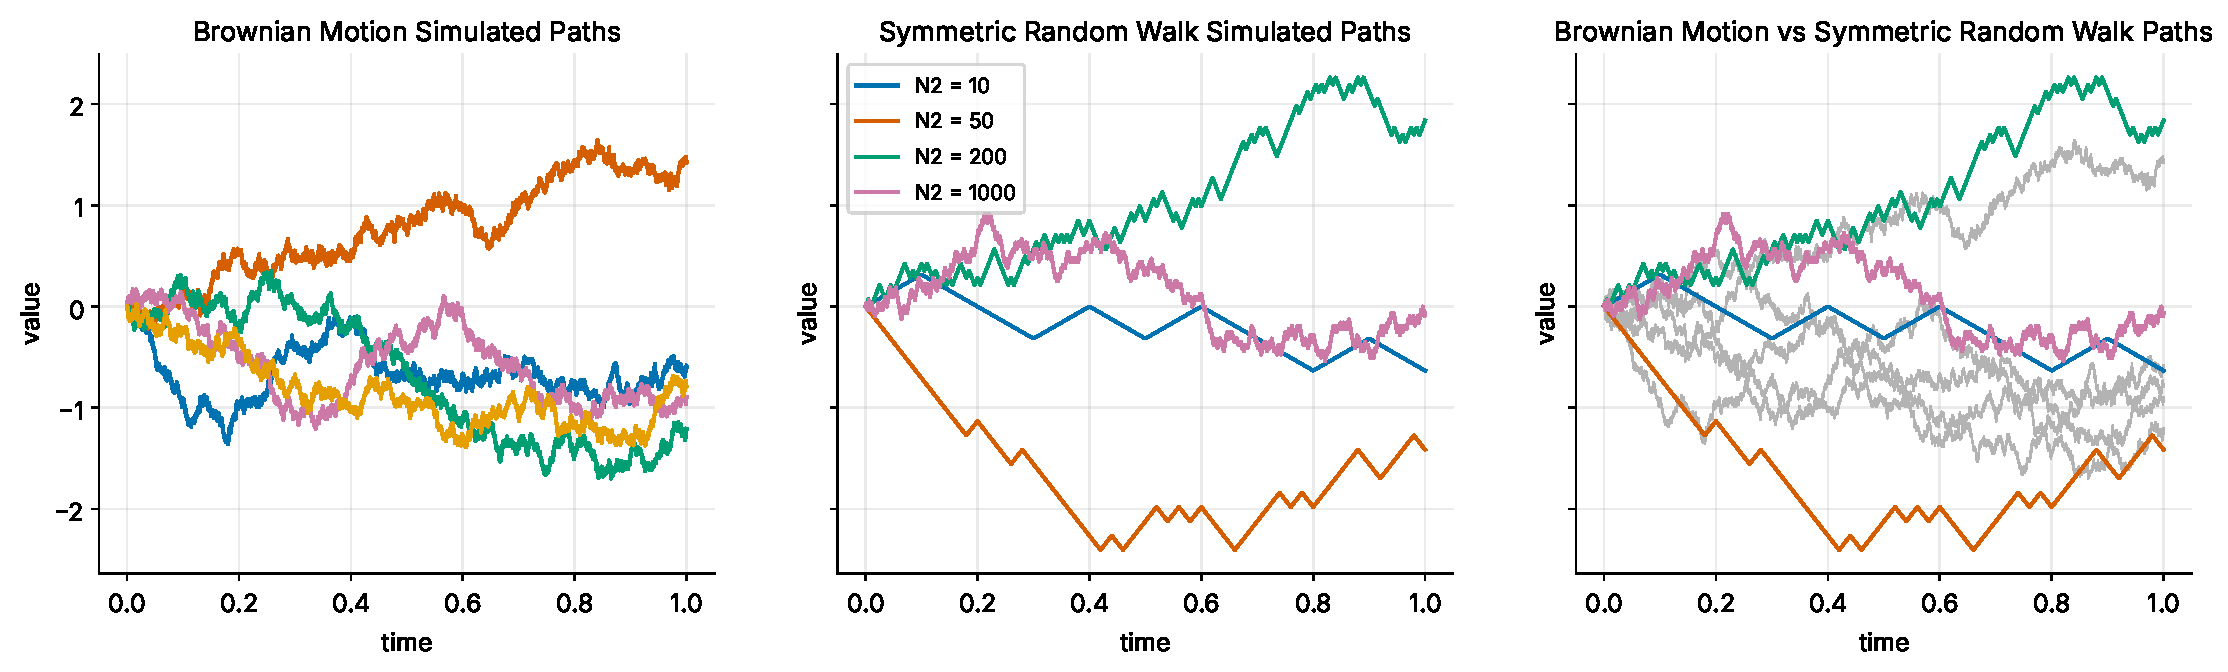
\includegraphics[width=\textwidth]{part1_paths.pdf}
\caption{Brownian motion paths ($N_1=10{,}000$; left), scaled symmetric random walks with $N_2=10,50,200,1000$ steps (middle) and both together (right).\label{fig:part1}}
\end{figure}

% P09 | 3 Part A: Brownian motion and random walks | Result: quadratic and total variation
% guide: dev_notes/paragraph_guides/P09_result_quadratic_and_total_variation.txt
The quadratic variation $\sum_k(\Delta W_k)^2$ of a Brownian path on $[0,1]$ is close to $1$ and its spread shrinks as $N$ grows; at $N=10{,}000$ the mean is \QVBMtenk.
For the scaled walk it equals $1$ exactly, because every squared step is $T/N$.
The total variation $\sum_k|\Delta W_k|$ does not converge: at $N=10{,}000$ it is \TVBMtenk\ for the Brownian paths, which matches the theoretical value \TVtheorytenk\ to the digits shown, and it equals $\sqrt N=100$ for the walk.
Table~\ref{tbl:variation} shows the same $\sqrt N$ growth at every $N$.
Infinite total variation means that $\int\sigma S\,dW$ cannot be defined path by path as an ordinary integral, which is why It\^o calculus is needed.
Finite and non-zero quadratic variation is what produces the correction $-\tfrac12\sigma^2$ in the drift of $\ln S_t$ in Section~\ref{sec:B-gbm}.
The same roughness explains why a hedge that is rebalanced only at discrete dates keeps a residual error (Section~\ref{sec:hedge}).


\begin{table}[h!]
\centering
\begin{tabular}{rccccc}
\toprule
$N$ & QV Brownian (sd) & QV walk & TV Brownian & TV walk & $\sqrt{2N/\pi}$ \\
\midrule
10 & 1.0092 (0.444) & 1.0000 & 2.54 & 3.16 & 2.52 \\
50 & 1.0074 (0.201) & 1.0000 & 5.66 & 7.07 & 5.64 \\
200 & 1.0028 (0.102) & 1.0000 & 11.30 & 14.14 & 11.28 \\
1,000 & 0.9974 (0.044) & 1.0000 & 25.20 & 31.62 & 25.23 \\
10,000 & 1.0000 (0.014) & 1.0000 & 79.79 & 100.00 & 79.79 \\
\bottomrule
\end{tabular}

\caption{Quadratic variation (QV) and total variation (TV) of the grid paths on $[0,1]$, 2000 paths per $N$. The entry in parentheses is the standard deviation of the QV.\label{tbl:variation}}
\end{table}

% P10 | 3 Part A: Brownian motion and random walks | Result: distance between the terminal laws
% guide: dev_notes/paragraph_guides/P10_result_distance_between_the_terminal_laws.txt
At $t=1$ the walk equals $(2B-N)/\sqrt N$ with $B\sim\mathrm{Bin}(N,\tfrac12)$, so its distribution function is a step function that is known exactly.
We therefore compute the Kolmogorov distance $\sup_x|F_N(x)-\Phi(x)|$ exactly, checking both sides of every jump, with no sampling error.
Table~\ref{tbl:ks} shows that the distance decreases like $N^{-1/2}$: the product of the distance and $\sqrt N$ settles at \KSconst\ as $N$ grows.
This constant is $1/\sqrt{2\pi}=\varphi(0)$, half the probability mass of the central lattice cell, which is the size of the jump of the distribution function at its mode.
The histograms of Figure~\ref{fig:rwhist} show the lattice structure at $N_2=10$ and an almost perfect bell shape from $N_2=200$ on.
The log--log plot in Figure~\ref{fig:ksrate} has slope $-\tfrac12$, in agreement with the Berry--Esseen bound.
The error in the law of the terminal value is of order $N^{-1/2}$, which is slower than the $O(1/N)$ error of the CRR call price in Section~\ref{sec:B}, because the price averages a Lipschitz payoff over the lattice.


\begin{table}[h!]
\centering
\begin{tabular}{rcc}
\toprule
$N_2$ & $\sup_x|F_{N_2}(x)-\Phi(x)|$ & $\times\sqrt{N_2}$ \\
\midrule
10 & 0.12305 & 0.389 \\
50 & 0.05614 & 0.397 \\
200 & 0.02817 & 0.398 \\
1,000 & 0.01261 & 0.399 \\
10,000 & 0.00399 & 0.399 \\
100,000 & 0.00126 & 0.399 \\
\bottomrule
\end{tabular}

\caption{Exact Kolmogorov distance between the law of the scaled walk at $t=1$ and $N(0,1)$.\label{tbl:ks}}
\end{table}

\begin{figure}[h!]
\centering
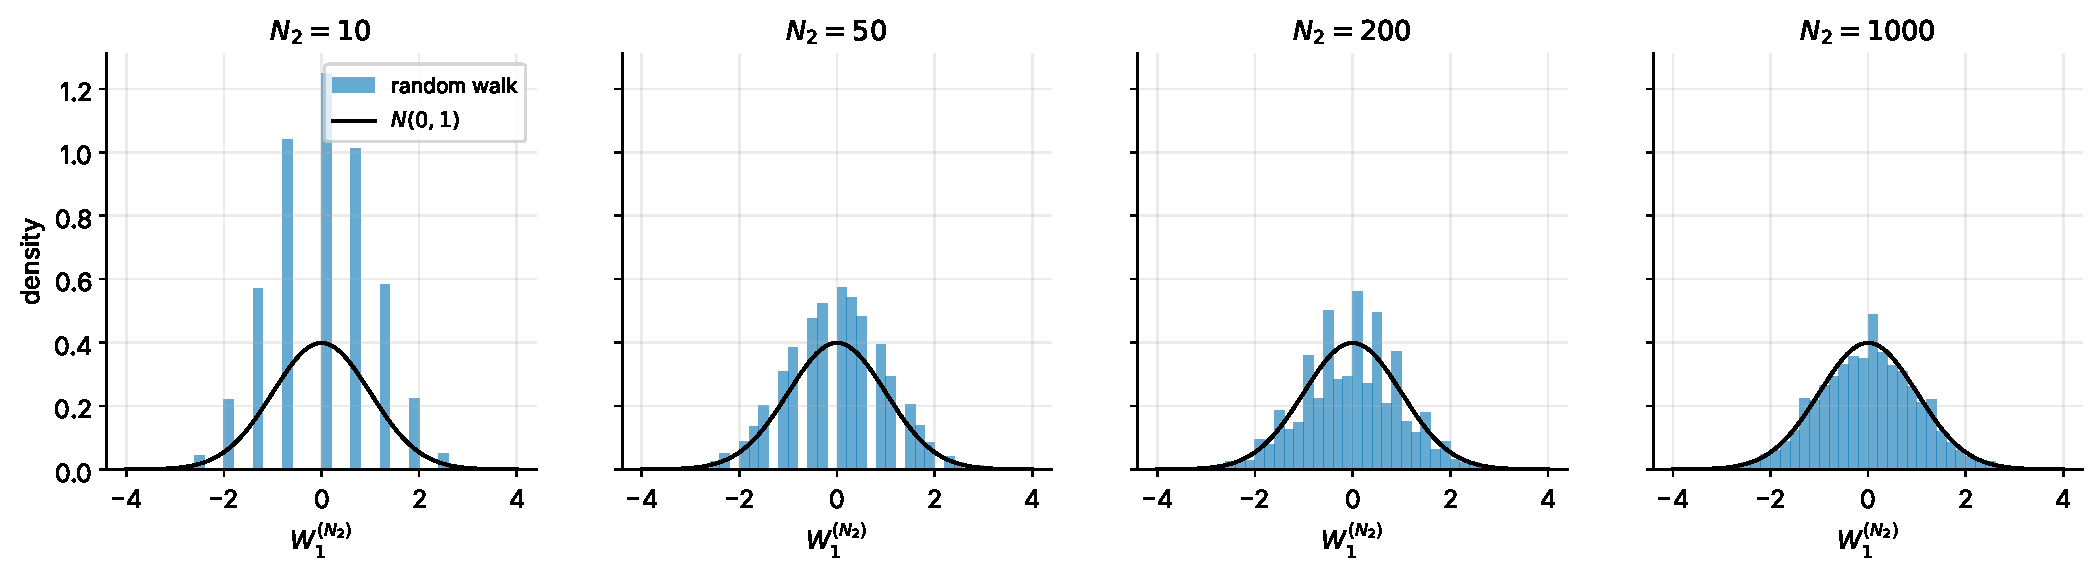
\includegraphics[width=\textwidth]{rw_terminal_hist.pdf}
\caption{Histogram of $W^{(N_2)}_1$ ($2\cdot10^4$ walks) against the $N(0,1)$ density.\label{fig:rwhist}}
\end{figure}

\begin{figure}[h!]
\centering
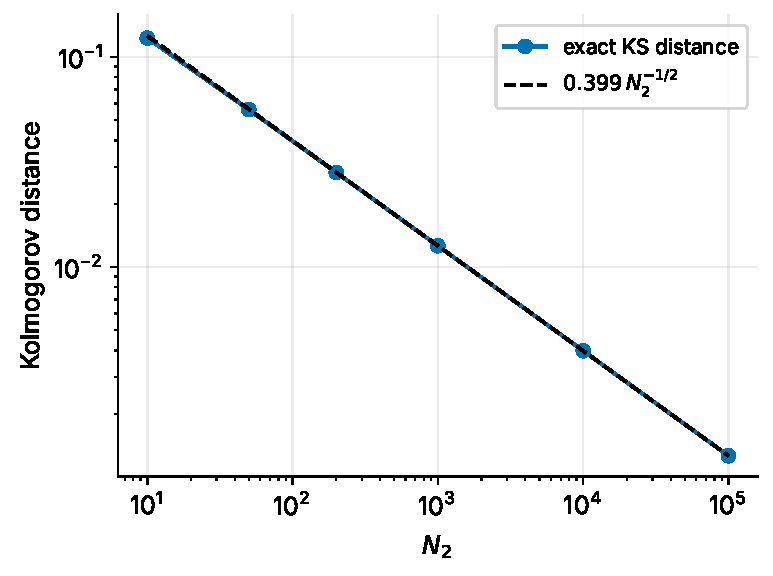
\includegraphics[width=0.45\textwidth]{ks_rate.pdf}
\caption{Kolmogorov distance against $N_2$ (log--log) with the limiting rate $0.399\,N_2^{-1/2}$.\label{fig:ksrate}}
\end{figure}

% P11 | 3 Part A: Brownian motion and random walks | Result: the running maximum and the reflection principle
% guide: dev_notes/paragraph_guides/P11_result_the_running_maximum_and_the_reflection_pr.txt
For a Brownian motion the reflection principle gives $\mathbb P(\max_{s\le1}W_s\ge a)=2\,(1-\Phi(a))$.
For the simple symmetric walk the same argument works exactly on the lattice and gives $\mathbb P(\max_{n\le N}S_n\ge k)=\mathbb P(S_N\ge k)+\mathbb P(S_N>k)$.
Figure~\ref{fig:runmax} shows that the survival function of the walk's maximum lies below the Brownian one, with a largest gap of \MaxGapTen\ at $N_2=10$ and \MaxGapTwoHundred\ at $N_2=200$.
The gap shrinks only like $N_2^{-1/2}$, the same slow rate as for the terminal law.
A discrete walk can cross a level only at a monitoring date, so it misses the excursions that happen between dates and its maximum is biased downwards.
The same bias appears whenever a path-dependent payoff is computed on a lattice or on a simulated grid.
For a barrier option this means that a tree or a simulation overstates the value of a knock-out and understates that of a knock-in unless the barrier is shifted by an amount of order $0.58\,\sigma\sqrt{\Delta t}$.


\begin{figure}[h!]
\centering
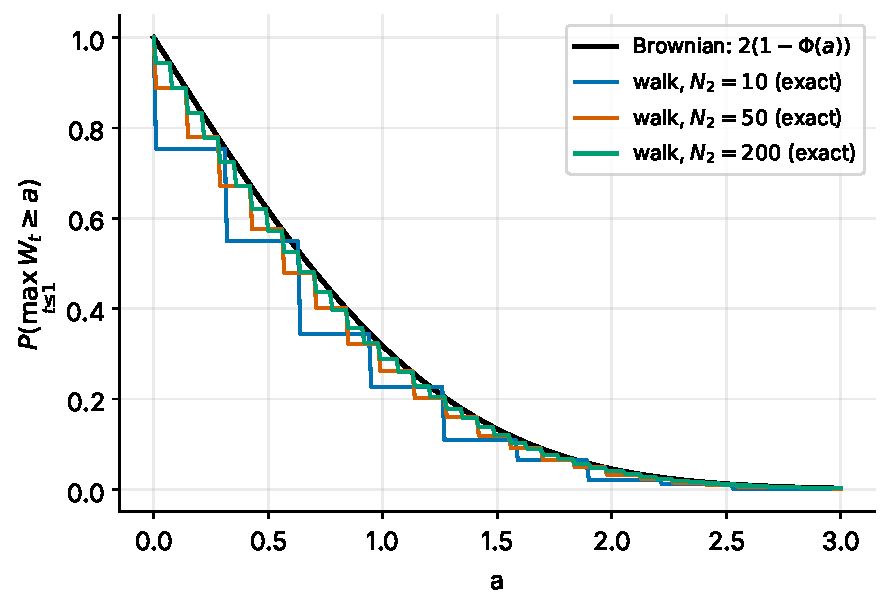
\includegraphics[width=0.62\textwidth]{running_max.pdf}
\caption{Survival function of the running maximum: exact for the walk (three values of $N_2$) and Brownian (reflection principle).\label{fig:runmax}}
\end{figure}
\FloatBarrier

% ======================================================================================== 4
\section{Part B: a European call on NVIDIA}\label{sec:B}

\subsection{The CRR model}\label{sec:B-crr}
% P12 | 4.1 CRR model | The CRR lattice and the risk-neutral probability
% guide: dev_notes/paragraph_guides/P12_the_crr_lattice_and_the_risk_neutral_probability.txt
Divide $[0,T]$ into $N$ steps of length $\Delta t=T/N$ and let the stock move in each step to $uS$ or $dS$ with $u=e^{\sigma\sqrt{\Delta t}}$ and $d=1/u$, so that after $j$ steps with $i$ up-moves the price is $S_{j,i}=S_0u^{2i-j}$.
Because $ud=1$ the tree recombines, layer $j$ has only $j+1$ nodes, and the choice of $u$ makes the variance of the one-step log-return equal to $\sigma^2\Delta t$.
No arbitrage forces the discounted stock to be a martingale under the pricing probability $p$ of an up-move, $S=e^{-r\Delta t}\big(p\,uS+(1-p)\,dS\big)$, which is solved by
\begin{equation}\label{eq:crrp}
 p=\frac{e^{r\Delta t}-d}{u-d},\qquad 0<p<1\iff d<e^{r\Delta t}<u,
\end{equation}
and the second condition holds for all small enough $\Delta t$.
To see why this is also a hedging price, choose a number of shares $\Delta$ and a bond holding $B$ with $\Delta uS+Be^{r\Delta t}=V_u$ and $\Delta dS+Be^{r\Delta t}=V_d$; subtracting gives $\Delta=\frac{V_u-V_d}{(u-d)S}$.
Substituting $p$ shows that the cost $\Delta S+B$ of this portfolio equals $e^{-r\Delta t}\big(pV_u+(1-p)V_d\big)$, so the price and the hedge are the same calculation.
The option tree is filled backward from the payoff $V_{N,i}=(S_{N,i}-K)^+$ with $V_{j,i}=e^{-r\Delta t}\big(pV_{j+1,i+1}+(1-p)V_{j+1,i}\big)$, and the price is $V_{0,0}$.
The class \texttt{CRRBinomialModel} stores every node, which costs $O(N^2)$ time and memory and is ideal for drawing trees and sample paths, whereas the vectorised pricer added for the experiments produces identical prices with $O(N)$ memory.


% P13 | 4.1 CRR model | Why the tree converges and why its error oscillates
% guide: dev_notes/paragraph_guides/P13_why_the_tree_converges_and_why_its_error_oscilla.txt
The terminal log-price of the tree is $\ln S_0+\sigma\sqrt{\Delta t}\,(2B-N)$ with $B\sim\mathrm{Bin}(N,p)$, a sum of $N$ independent steps.
By the central limit theorem it converges to a normal law with mean $\ln S_0+(r-\tfrac12\sigma^2)T$ and variance $\sigma^2T$, which is the law of $\ln S_T$ under geometric Brownian motion, so the tree price converges to the Black--Scholes price.
The error of the tree price is of order $1/N$, but it is not monotone in $N$.
With $K=S_0$ a terminal node sits exactly at the strike when $N$ is even and the kink falls half-way between two nodes when $N$ is odd, so the error behaves like $(-1)^Nc/N$ rather than $c/N$.
Four standard remedies are compared in Section~\ref{sec:B-quality}: averaging the prices for $N$ and $N+1$ steps; Broadie--Detemple smoothing, which replaces the last layer by the Black--Scholes value of the one-step claim; Richardson extrapolation $2V_{2N}-V_N$; and the Leisen--Reimer tree, which is built so that the strike coincides with a node boundary.
The first three remove the oscillation and the Leisen--Reimer tree additionally raises the order of convergence from one to two.
Accelerations that use a closed form at the last step apply only to European payoffs, so for the American put of Part C we keep the plain CRR lattice and control the error by refinement and extrapolation.


\subsection{Geometric Brownian motion and its simulation}\label{sec:B-gbm}
% P14 | 4.2 GBM and simulation | Geometric Brownian motion and its discretisations
% guide: dev_notes/paragraph_guides/P14_geometric_brownian_motion_and_its_discretisation.txt
Applying It\^o's formula to $f(S)=\ln S$, with $f'=1/S$ and $f''=-1/S^2$, gives $d\ln S_t=\frac{dS_t}{S_t}-\frac12\frac{(dS_t)^2}{S_t^2}=(\mu-\tfrac12\sigma^2)\,dt+\sigma\,dW_t$, hence
\begin{equation}\label{eq:gbmsol}
 S_t=S_0\exp\!\Big((\mu-\tfrac12\sigma^2)t+\sigma W_t\Big).
\end{equation}
Hence $S_t$ is lognormal, strictly positive, with $\mathbb E[S_t]=S_0e^{\mu t}$.
Under $\mathbb Q$ the drift $\mu$ is replaced by $r$, and the call is priced as $e^{-rT}\,\mathbb E[(S_T-K)^+]$, estimated by a Monte Carlo average over simulated terminal values.
The Euler--Maruyama scheme updates $S_{n+1}=S_n+\mu S_n\Delta t+\sigma S_n\Delta W_n$, which is cheap and generic but can in principle produce negative prices, whereas the exact step $S_{n+1}=S_n\exp\big((\mu-\tfrac12\sigma^2)\Delta t+\sigma\sqrt{\Delta t}\,Z_n\big)$ keeps the price positive and has no discretisation error.
Both are driven by the same random numbers in Figure~\ref{fig:gbm}, so any difference between the two panels is discretisation error alone.
The functions \texttt{gbm\_euler\_maruyama} and \texttt{gbm\_exact} return full paths, which is what the figures need.
For the price tables we add a version that keeps only the current vector of prices, because $5\cdot10^5$ paths with 300 steps would otherwise occupy more than a gigabyte, and we check that it reproduces the original function when both receive the same random numbers.


\subsection{The Black--Scholes benchmark and the Greeks}\label{sec:B-bs}
% P15 | 4.3 Black-Scholes benchmark | The Black-Scholes formula and the Greeks
% guide: dev_notes/paragraph_guides/P15_the_black_scholes_formula_and_the_greeks.txt
Evaluating $e^{-rT}\mathbb E^{\mathbb Q}[(S_T-K)^+]$ for the lognormal $S_T$ gives
\begin{equation}\label{eq:bs}
 C=S_0\Phi(d_1)-Ke^{-rT}\Phi(d_2),\qquad d_{1,2}=\frac{\ln(S_0/K)+(r\pm\frac12\sigma^2)T}{\sigma\sqrt T},
\end{equation}
and the put follows from put--call parity $C-P=S_0-Ke^{-rT}$.
The sensitivities are $\Delta=\Phi(d_1)$, $\Gamma=\varphi(d_1)/(S_0\sigma\sqrt T)$, $\mathcal V=S_0\varphi(d_1)\sqrt T$, $\rho=KTe^{-rT}\Phi(d_2)$ and $\Theta=-\frac{S_0\varphi(d_1)\sigma}{2\sqrt T}-rKe^{-rT}\Phi(d_2)$, where $\varphi$ is the standard normal density.
For the NVIDIA call they take the values $\Delta=\BSdelta$, $\Gamma=\BSgamma$, vega $\BSvega$ (that is, \BSvegaPct\ dollars per volatility point), $\Theta=\BStheta$ per year and $\rho=\BSrho$.
Delta is the number of shares that hedges the option, gamma measures how quickly that number changes and therefore how large the hedging error is when rebalancing is discrete, and vega is the exposure to the volatility input, which is the least certain one.
Theta is the loss of value from the passage of time alone, about \BSthetaDay\ dollars per calendar day at the money, and rho the exposure to the interest rate.
The price \$\BSprice\ from Equation~\eqref{eq:bs} is the reference against which every numerical estimate in this part is measured.


\begin{figure}[h!]
\centering
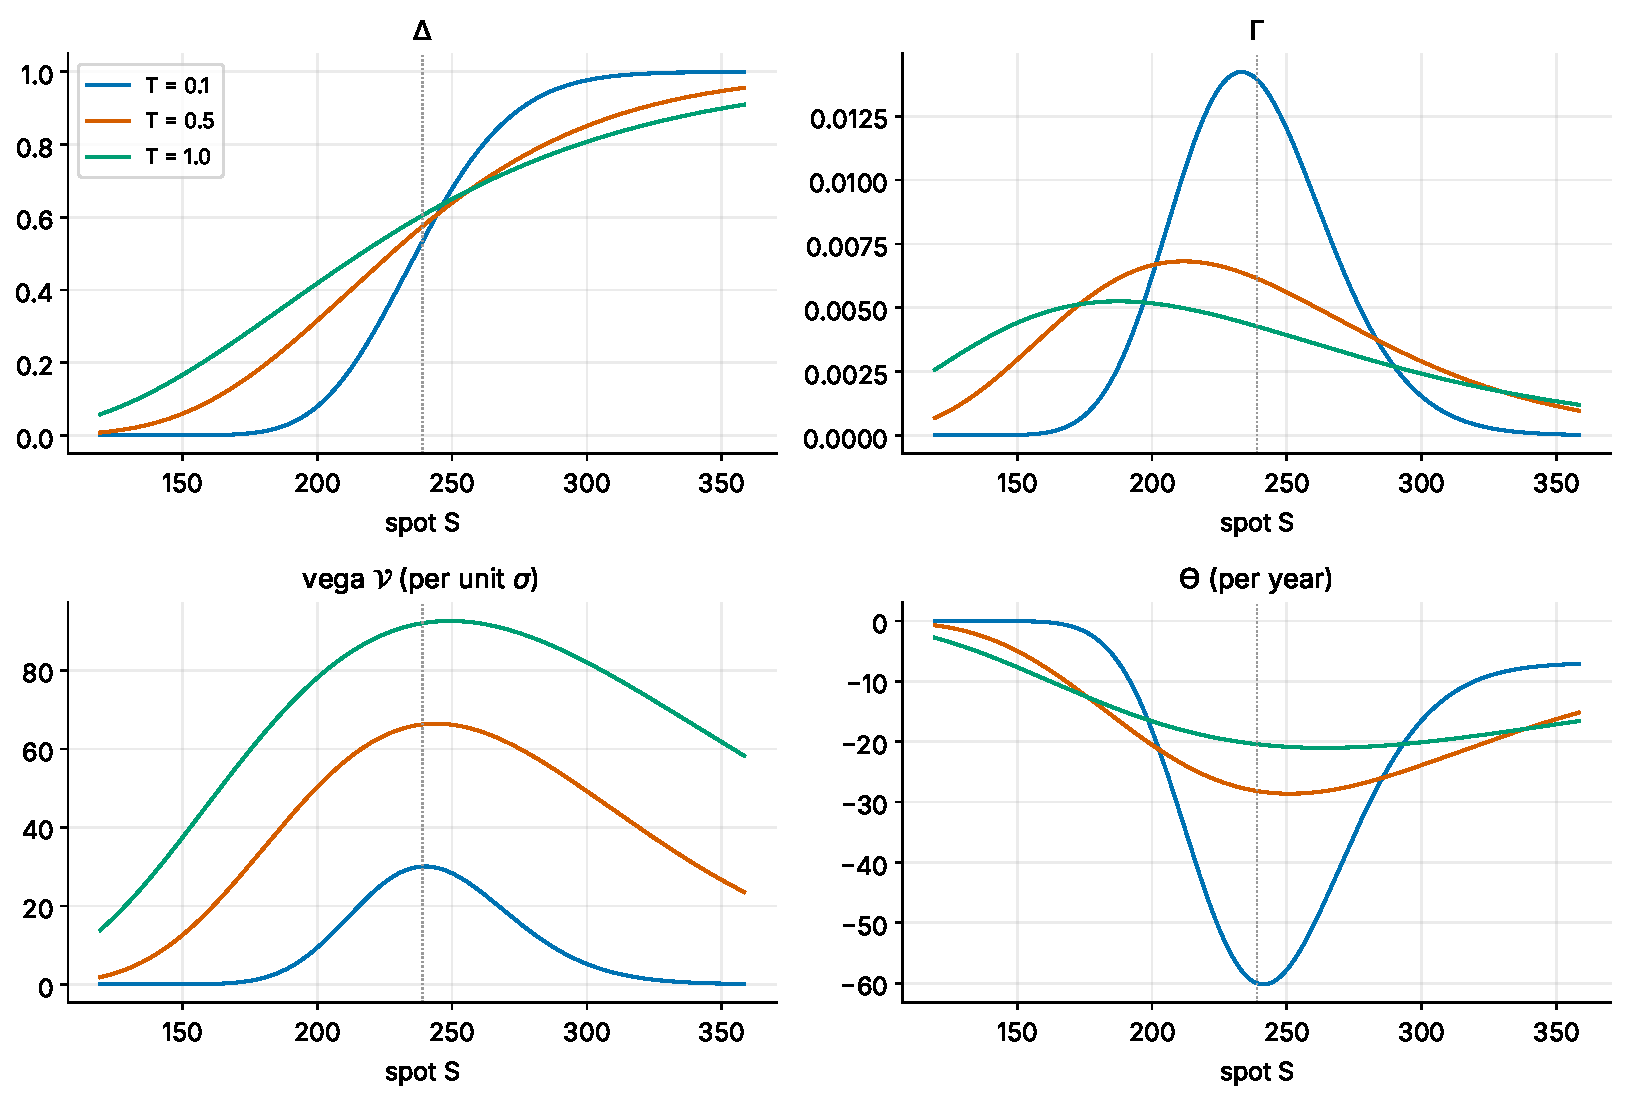
\includegraphics[width=0.85\textwidth]{bs_greeks.pdf}
\caption{Black--Scholes Greeks of the call against spot for three maturities ($K=238.90$, $r=\NvdaR\%$, $\sigma=\NvdaSigma\%$).\label{fig:bsgreeks}}
\end{figure}

\begin{figure}[h!]
\centering
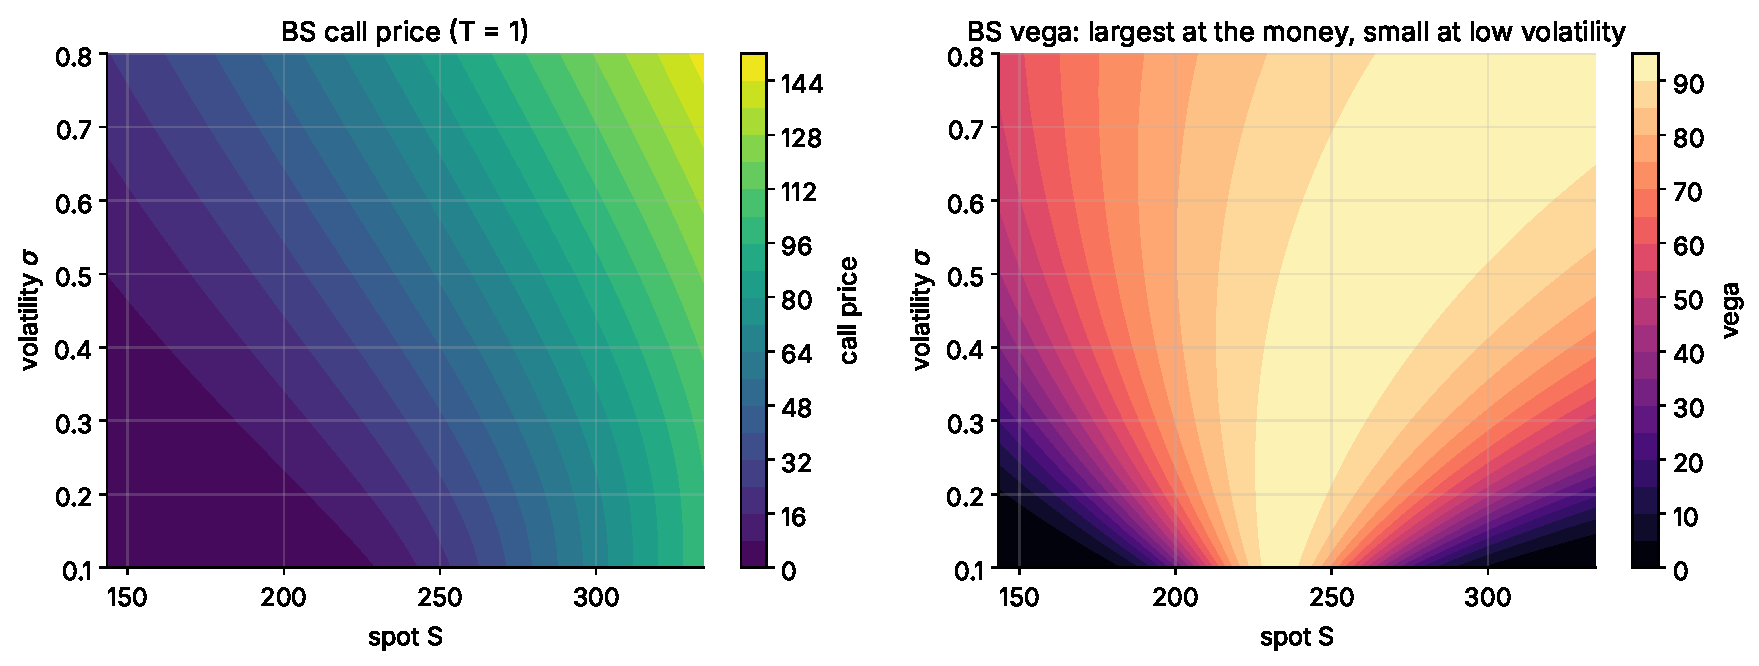
\includegraphics[width=0.95\textwidth]{bs_surface.pdf}
\caption{Black--Scholes call price (left) and vega (right) as functions of spot and volatility ($T=1$).\label{fig:bssurface}}
\end{figure}

\subsection{Results: sample paths and binomial prices}\label{sec:B-prices}
% P16 | 4.4 Results | Result: sample paths in the tree and in GBM
% guide: dev_notes/paragraph_guides/P16_result_sample_paths_in_the_tree_and_in_gbm.txt
Figure~\ref{fig:binpaths} shows five stock paths and five option-value paths in the tree with $N=100$, simulated with the risk-neutral probability $p$.
The stock paths fan out like a random walk with drift $r$, and at this resolution the lattice is no longer visible.
The option value follows the stock but is a convex function of it, so it moves faster than the stock when the call is in the money and flattens when it is out of the money.
Every path of the option value ends at the payoff $(S_T-K)^+$.
Figure~\ref{fig:gbm} compares Euler--Maruyama with the exact solution for the same random numbers and $N=2000$ steps.
The two panels are indistinguishable by eye, and the largest difference between a pair of paths is about a dollar on a price of $\$240$.
These figures say nothing about the accuracy of prices, which is the subject of the tables that follow.


\begin{figure}[h!]
\centering
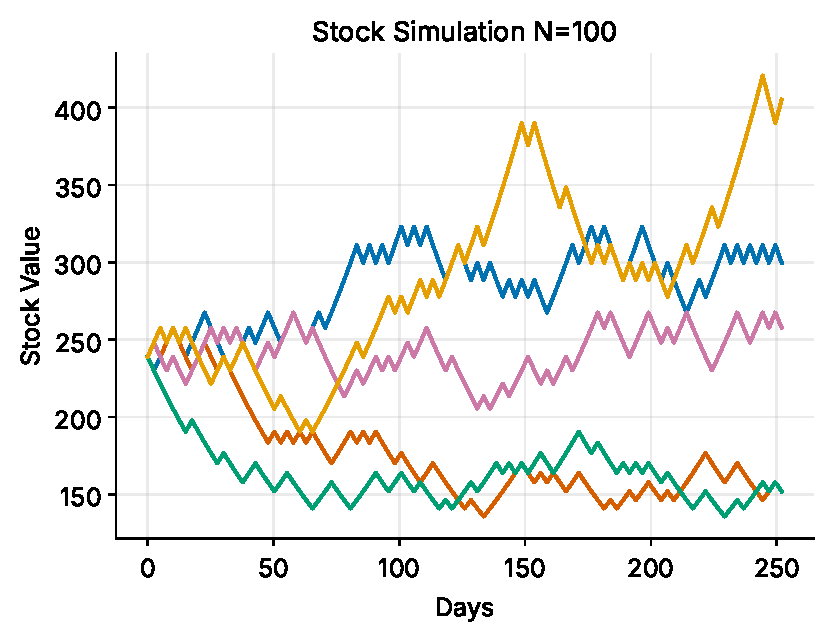
\includegraphics[width=0.48\textwidth]{simulate_stocks.pdf}\hfill
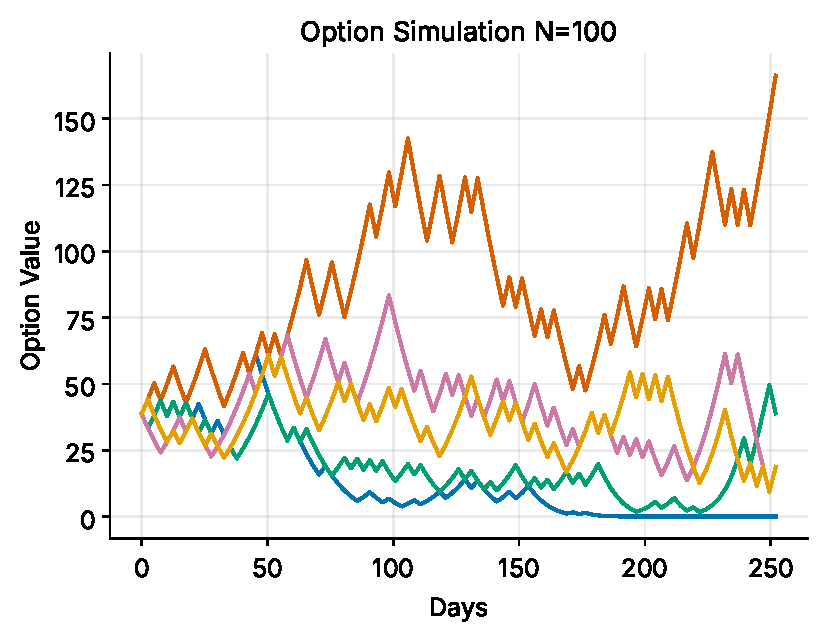
\includegraphics[width=0.48\textwidth]{simulate_options.pdf}
\caption{Five simulated stock (left) and option (right) value paths in the CRR tree, $N=100$.\label{fig:binpaths}}
\end{figure}

\begin{figure}[h!]
\centering
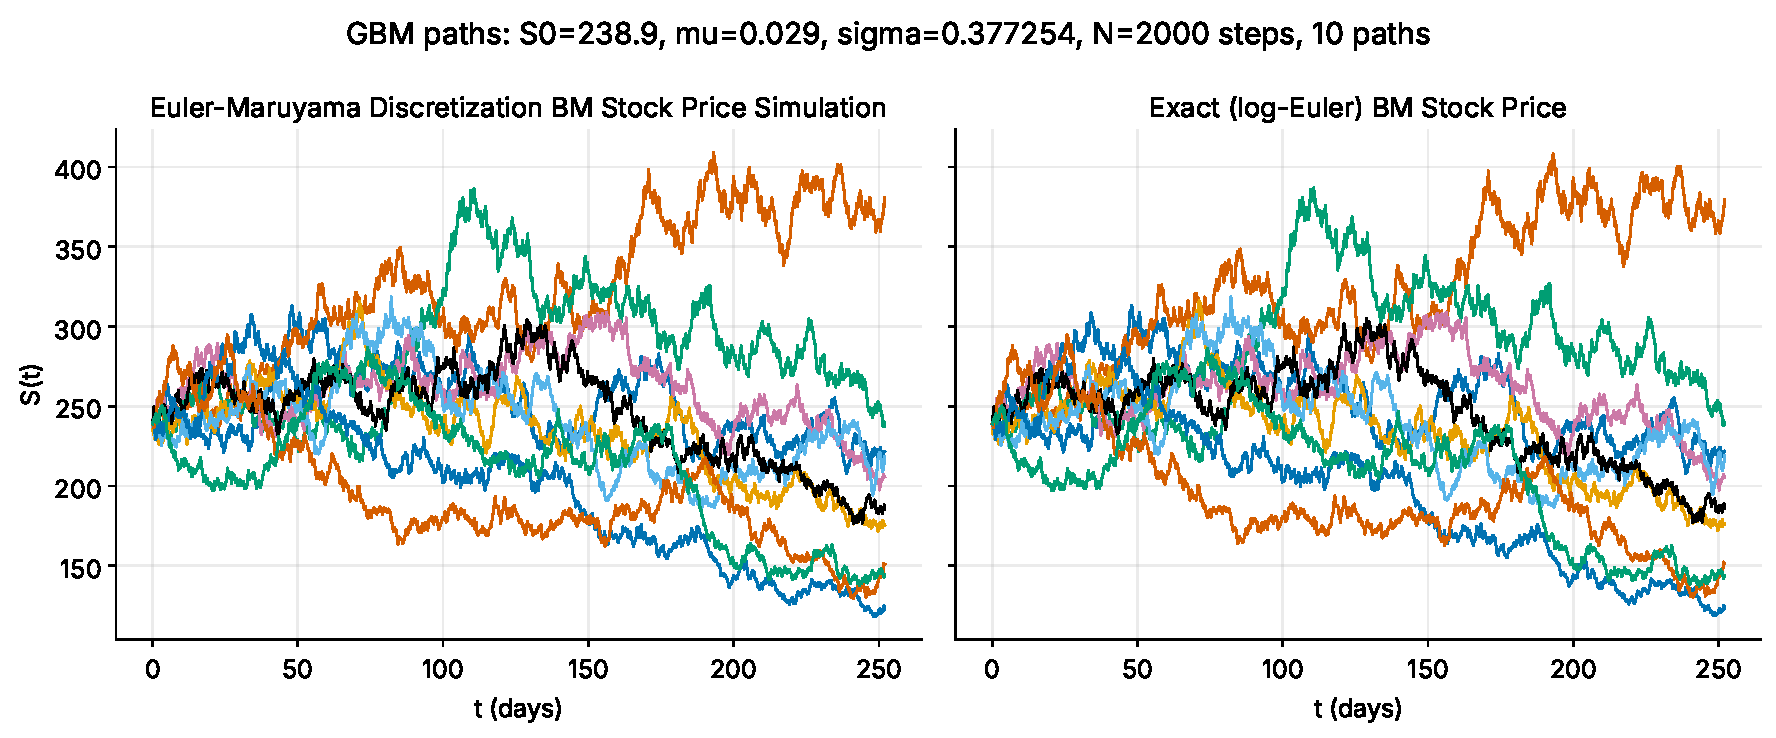
\includegraphics[width=\textwidth]{gbm_paths.pdf}
\caption{GBM paths with Euler--Maruyama (left) and exact (right) simulation, same random numbers.\label{fig:gbm}}
\end{figure}

% P17 | 4.4 Results | Result: binomial prices against Black-Scholes
% guide: dev_notes/paragraph_guides/P17_result_binomial_prices_against_black_scholes.txt
The CRR price converges to the Black--Scholes price of \$\BSprice: at $N=10{,}000$ it is \$\CRRtenk, an error of \$\CRRtenkErr.
The error is \$\CRRhundredErr\ at $N=100$ and \$\CRRthousandErr\ at $N=1000$, so one hundred steps already give the price to within ten cents.
The last column of Table~\ref{tbl:bin} shows that $N$ times the absolute error is nearly constant from $N=50$ on.
This is first-order convergence, as predicted in Section~\ref{sec:B}.
For small $N$ the error alternates in sign: the tree overprices the call at $N=5$ and $N=25$ and underprices it at $N=10$ and $N=50$.
This is the parity effect of the kink at the strike and is quantified in the next section.
The row for $N=10{,}000$ was computed with the vectorised pricer, since the list-based class would have to store about $5\cdot10^{7}$ nodes.


\begin{table}[h!]
\centering
\begin{tabular}{rccc}
\toprule
$N$ & CRR price & $|\mathrm{CRR}-\mathrm{BS}|$ & $N\times|\mathrm{error}|$ \\
\midrule
5 & 40.4839 & 1.7347 & 8.673 \\
10 & 37.8785 & 0.8708 & 8.708 \\
25 & 39.0918 & 0.3425 & 8.562 \\
50 & 38.5731 & 0.1762 & 8.809 \\
100 & 38.6611 & 0.0882 & 8.820 \\
200 & 38.7051 & 0.0441 & 8.826 \\
500 & 38.7316 & 0.0177 & 8.829 \\
1,000 & 38.7404 & 0.0088 & 8.831 \\
10,000 & 38.7484 & 0.0009 & 8.832 \\
\bottomrule
\end{tabular}

\caption{CRR prices of the one-year call against the Black--Scholes price. $N\le1000$ with the list-based class, $N=10{,}000$ with the vectorised pricer.\label{tbl:bin}}
\end{table}

\subsection{Quality of the binomial price: the saw-tooth and faster trees}\label{sec:B-quality}
% P18 | 4.5 Tree quality | Result: the saw-tooth and the faster trees
% guide: dev_notes/paragraph_guides/P18_result_the_saw_tooth_and_the_faster_trees.txt
Figure~\ref{fig:saw} shows that the signed error alternates with the parity of $N$: $N$ times the error settles at $\SawEven$ for even $N$ and at $\SawOdd$ for odd $N$.
In absolute value both sequences decay like $1/N$, so parity changes the sign of the error but not its order.
Table~\ref{tbl:variants} compares seven trees at odd $N$.
At $N=101$ the Leisen--Reimer tree has an error of \LRerrHundred\ against \CRRerrHundredOdd\ for plain CRR, and at $N=1001$ its error is \LRerrThousand.
On the log--log plot of Figure~\ref{fig:variants} plain CRR, Jarrow--Rudd and Tian follow slope $-1$ with visible oscillation, while averaging and smoothing remove most of the oscillation.
Only the Leisen--Reimer tree changes the slope, to $-2$.
For a European payoff with a kink the practical choice is therefore the Leisen--Reimer tree or smoothing combined with Richardson extrapolation.
For an American payoff we stay with plain CRR and control the error by refinement, because the accelerations rely on a closed-form value at the last step.


\begin{figure}[h!]
\centering
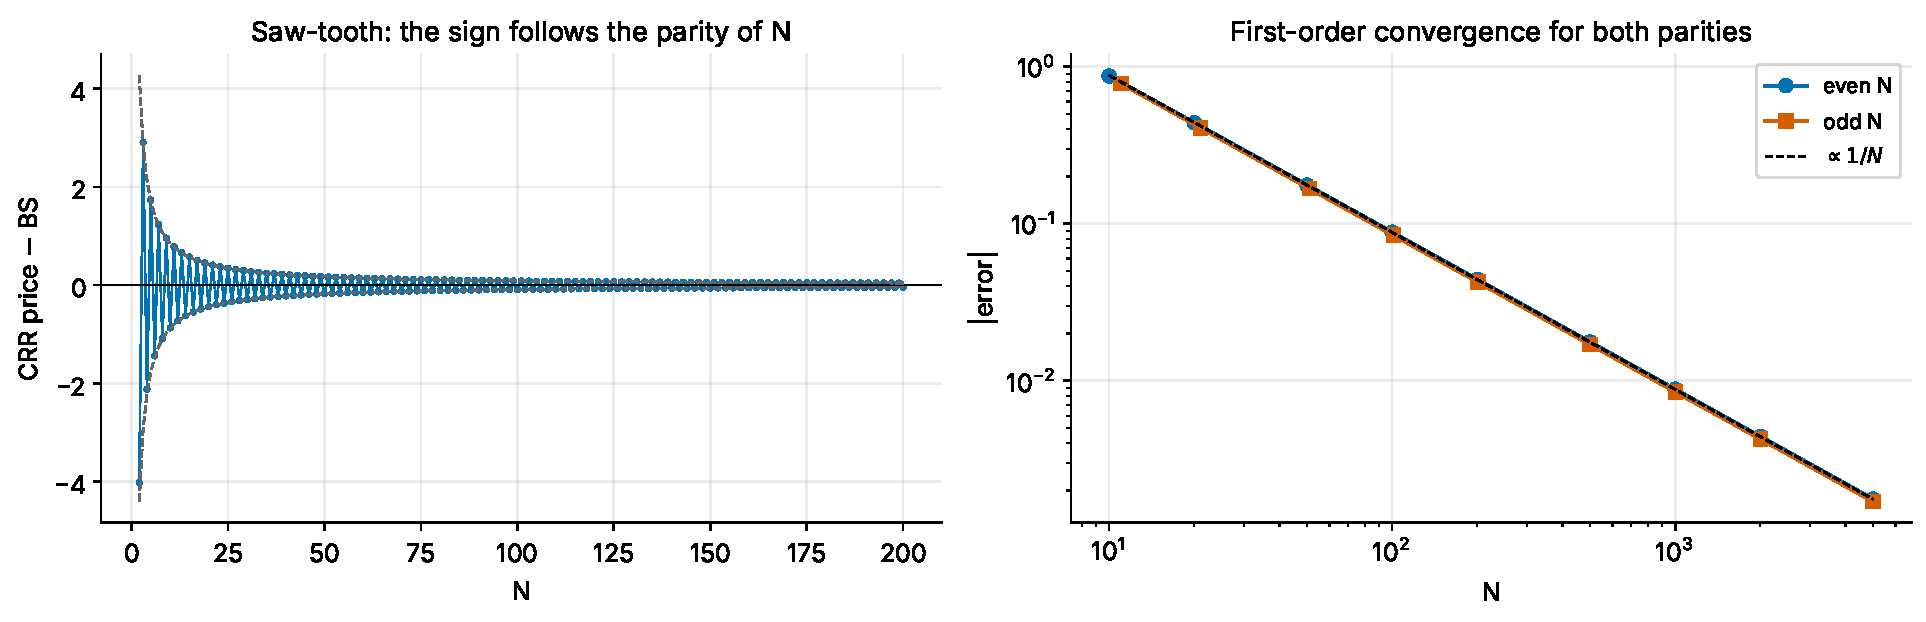
\includegraphics[width=\textwidth]{crr_sawtooth.pdf}
\caption{Left: signed CRR error for $N=2,\dots,200$ with the envelopes $c_{even}/N$ and $c_{odd}/N$. Right: absolute error for even and odd $N$ (log--log).\label{fig:saw}}
\end{figure}

\begin{figure}[h!]
\centering
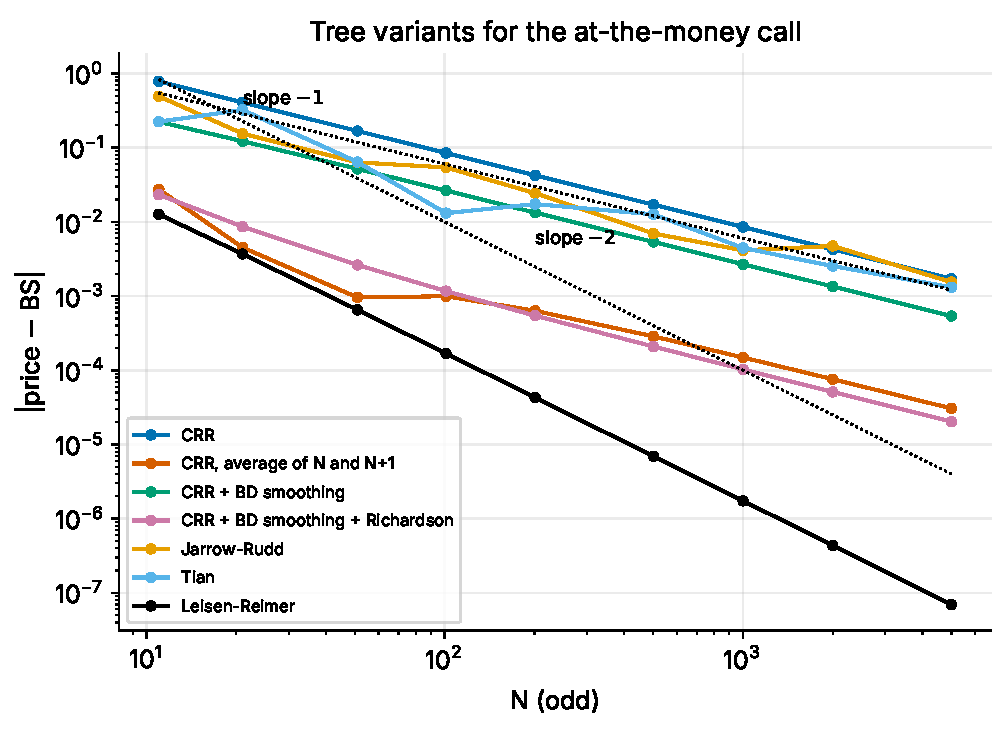
\includegraphics[width=0.62\textwidth]{tree_variants.pdf}
\caption{Absolute error of seven tree variants at odd $N$ (log--log).\label{fig:variants}}
\end{figure}

\begin{table}[h!]
\centering
\begin{tabular}{lcccc}
\toprule
Tree / acceleration & $N=21$ & $N=101$ & $N=501$ & $N=2001$ \\
\midrule
CRR & 4.1e-01 & 8.4e-02 & 1.7e-02 & 4.3e-03 \\
CRR, average of N and N+1 & 4.5e-03 & 9.9e-04 & 2.9e-04 & 7.6e-05 \\
CRR + BD smoothing & 1.2e-01 & 2.6e-02 & 5.4e-03 & 1.3e-03 \\
CRR + BD smoothing + Richardson & 8.6e-03 & 1.2e-03 & 2.1e-04 & 5.1e-05 \\
Jarrow-Rudd & 1.5e-01 & 5.4e-02 & 7.0e-03 & 4.7e-03 \\
Tian & 3.2e-01 & 1.3e-02 & 1.3e-02 & 2.5e-03 \\
Leisen-Reimer & 3.7e-03 & 1.7e-04 & 6.9e-06 & 4.4e-07 \\
\bottomrule
\end{tabular}

\caption{Absolute error of the tree variants for selected odd $N$.\label{tbl:variants}}
\end{table}
\FloatBarrier

\subsection{Monte Carlo}\label{sec:B-mc}
% P19 | 4.6 Monte Carlo | Result: Monte Carlo prices by paths and steps
% guide: dev_notes/paragraph_guides/P19_result_monte_carlo_prices_by_paths_and_steps.txt
With $5\cdot10^5$ paths and $N=300$ steps the Euler--Maruyama Monte Carlo price is \$\MCbest\ with standard error \$\MCbestSE, which is within \$\MCbestErr\ of the Black--Scholes price.
The other two step counts at the same sample size are closer to the benchmark, so the ordering of the cells in the last row is noise: all three lie within about a third of a standard error of each other.
With only 1,000 paths the standard error is above two dollars, about six percent of the price, and the errors in that row are of this size.
They are statistical fluctuations, not systematic bias, since they change sign across columns.
Increasing the number of time steps from 100 to 300 changes the price by much less than its standard error.
The statistical error therefore dominates the Euler bias at these step counts, in line with the weak order of the scheme.
Because the standard error falls only like $M^{-1/2}$, a standard error of one cent would need about $5\cdot10^{9}$ paths, whereas the tree reaches that accuracy deterministically with a few thousand steps.


\begin{table}[h!]
\centering
\begin{tabular}{rccc}
\toprule
Paths & $N=100$ & $N=200$ & $N=300$ \\
\midrule
1,000 & 41.4717 (2.325) & 38.7524 (2.097) & 41.2796 (2.218) \\
10,000 & 38.5516 (0.681) & 39.3903 (0.695) & 39.8024 (0.698) \\
100,000 & 38.8126 (0.215) & 38.6919 (0.216) & 38.7307 (0.216) \\
250,000 & 38.8783 (0.136) & 38.9348 (0.137) & 38.6022 (0.136) \\
500,000 & 38.7540 (0.096) & 38.7559 (0.096) & 38.7236 (0.096) \\
\bottomrule
\end{tabular}

\caption{Euler--Maruyama Monte Carlo prices of the call, price (standard error), for $N$ time steps and the number of paths in the first column.\label{tbl:mc}}
\end{table}

% P20 | 4.6 Monte Carlo | Result: strong and weak order of Euler-Maruyama
% guide: dev_notes/paragraph_guides/P20_result_strong_and_weak_order_of_euler_maruyama.txt
The strong error $\mathbb E|S^{EM}_T-S_T|$ compares each Euler path with the exact path driven by the same noise, whereas the weak error compares the expectation of a payoff and is the only one that matters for pricing.
We measure both with common random numbers, so the Monte Carlo noise in the difference is small.
The strong error falls from $0.069$ at $N=1$ to $0.0052$ at $N=256$ (in units of $S_0$), and the log--log slope is \EMstrongSlope, which is order one half.
This is the textbook strong order of the Euler--Maruyama scheme.
The bias of the call price halves each time $N$ doubles between $N=4$ and $N=64$, with a log--log slope of \EMweakSlope, which is weak order one.
At $N=256$ the bias is $+0.0066$ with a standard error of $0.0022$, so it can no longer be separated from zero.
For a European call a few hundred steps are therefore enough and the number of paths is the decision that matters; at $N=1$ the bias even has the opposite sign, which is a pre-asymptotic effect.


\begin{table}[h!]
\centering
\begin{tabular}{rccc}
\toprule
$N$ & $\mathbb E|S_T^{\rm EM}-S_T|/S_0$ & price bias & (s.e.) \\
\midrule
1 & 0.0692 & -0.3169 & (0.0323) \\
2 & 0.0534 & +0.3639 & (0.0226) \\
4 & 0.0395 & +0.3603 & (0.0163) \\
8 & 0.0286 & +0.2208 & (0.0119) \\
16 & 0.0205 & +0.1103 & (0.0086) \\
32 & 0.0146 & +0.0566 & (0.0061) \\
64 & 0.0103 & +0.0255 & (0.0044) \\
128 & 0.0073 & +0.0178 & (0.0031) \\
256 & 0.0052 & +0.0066 & (0.0022) \\
\bottomrule
\end{tabular}

\caption{Strong error and weak error (call-price bias) of Euler--Maruyama, $4\cdot10^5$ paths with common random numbers.\label{tbl:em}}
\end{table}

\begin{figure}[h!]
\centering
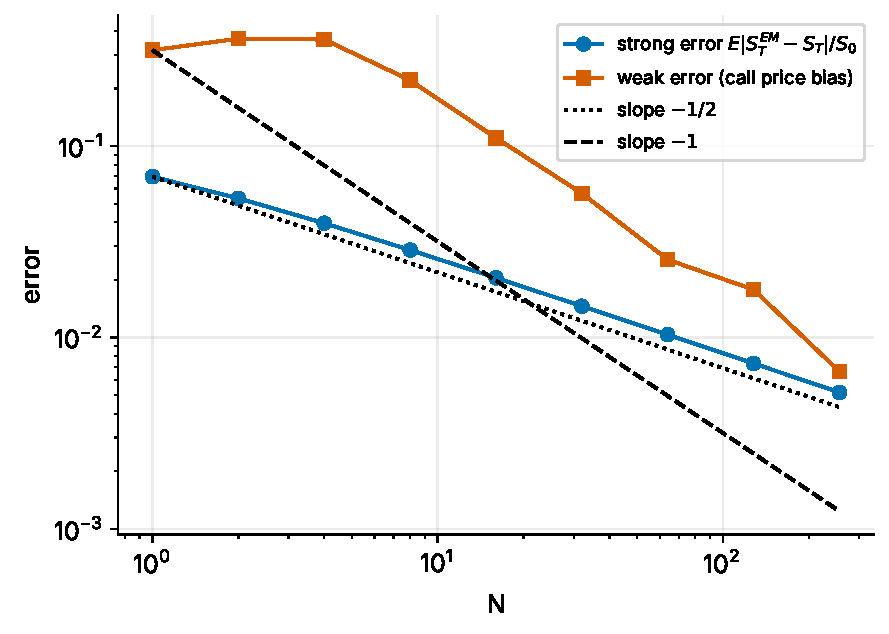
\includegraphics[width=0.5\textwidth]{em_order.pdf}
\caption{Strong and weak error of Euler--Maruyama against $N$ (log--log).\label{fig:emorder}}
\end{figure}

% P21 | 4.6 Monte Carlo | Result: variance reduction
% guide: dev_notes/paragraph_guides/P21_result_variance_reduction.txt
At $M=\VRM$ samples the antithetic estimator reduces the variance of the plain estimator by a factor of \VRanti\ and the control variate by a factor of \VRcv.
Scrambled Sobol quasi-Monte Carlo reduces it by a factor of \VRsobol, which is why it nearly disappears from the log--log plot of Figure~\ref{fig:vr}.
The control variate uses the discounted terminal price, whose expectation $S_0$ is known exactly and which is strongly correlated with the call payoff near the money.
The coefficient of the correction is estimated from the same sample, which introduces a negligible bias.
Quasi-Monte Carlo is so effective here because the integrand is a function of a single uniform variable, for which low-discrepancy points give an error close to $1/M$.
A path-dependent payoff depends on one random number per time step, and the advantage shrinks as this dimension grows unless a Brownian-bridge construction concentrates the variance in the first coordinates.
The standard errors are trustworthy: the 95\% intervals of the plain estimator cover the Black--Scholes price in \MCcoverage\% of 400 repetitions.
Simulating with a real-world drift of $10\%$ instead of $r$ would give a price of \$\WrongMuPrice\ instead of \$\BSprice, which is the classical error of pricing under the wrong measure.


\begin{table}[h!]
\centering
\begin{tabular}{lcccc}
\toprule
Method & mean estimate & sd of estimates & RMSE & variance ratio vs plain \\
\midrule
plain & 38.7455 & 0.1228 & 0.1213 & 1.0 \\
antithetic & 38.7763 & 0.0921 & 0.0949 & 1.8 \\
control variate & 38.7491 & 0.0441 & 0.0436 & 7.7 \\
Sobol (scrambled) & 38.7494 & 0.0004 & 0.0005 & 76726.6 \\
\bottomrule
\end{tabular}

\caption{Variance reduction at $M=262{,}144$ samples, 40 repetitions. The last column is the variance of the plain estimator divided by that of the method.\label{tbl:vr}}
\end{table}

\begin{figure}[h!]
\centering
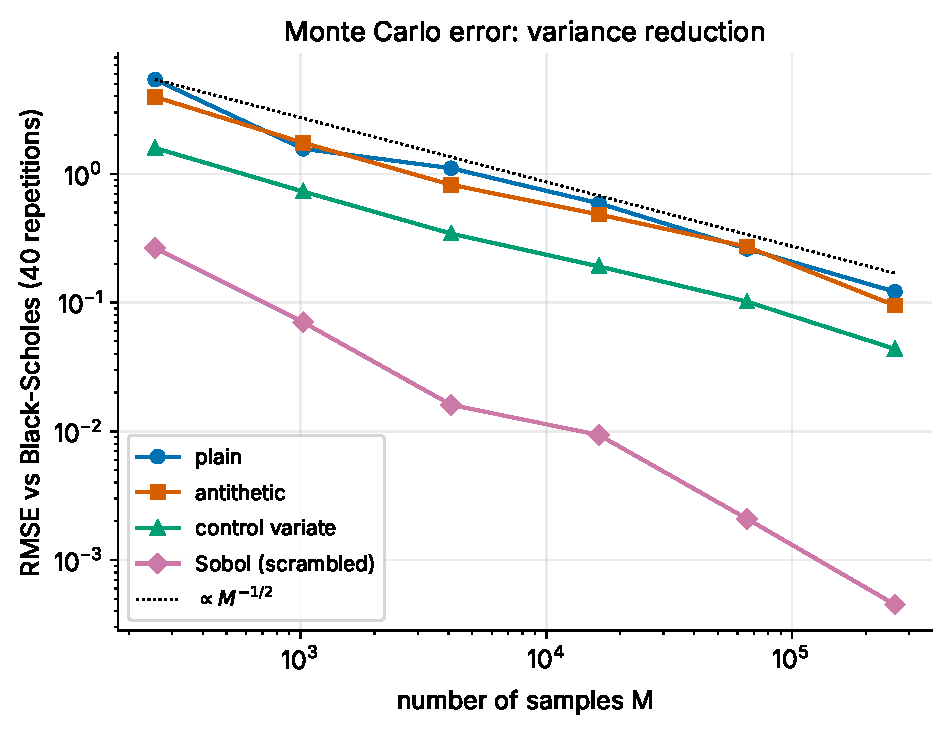
\includegraphics[width=0.55\textwidth]{mc_variance_reduction.pdf}
\caption{RMSE of four Monte Carlo estimators against the number of samples (log--log).\label{fig:vr}}
\end{figure}
\FloatBarrier

\subsection{Greeks by three routes}\label{sec:B-greeks}
% P22 | 4.7 Greeks | Result: Greeks from three routes
% guide: dev_notes/paragraph_guides/P22_result_greeks_from_three_routes.txt
Table~\ref{tbl:greeks} shows that all routes agree: $\Delta$ is \BSdelta\ from Black--Scholes, \TreeDelta\ from the tree and \MCdeltaPW\ from the pathwise Monte Carlo estimator.
The tree obtains $\Delta$ and $\Gamma$ for free from its first two layers, while vega and rho need a bump of the inputs.
For $\Gamma$ the tree gives \TreeGamma\ and the Monte Carlo estimator that combines the pathwise and likelihood-ratio ideas gives \MCgammaLR\ with standard error \MCgammaLRSE.
A bump-and-revalue estimator with common random numbers has a standard error of \MCgammaBumpSE, which is larger because the second difference divides the noise by the square of the bump size.
For vega the pathwise estimator has a smaller standard error than the likelihood-ratio estimator, because it differentiates the payoff, which is Lipschitz, instead of the density.
The likelihood-ratio method earns its place when the payoff is too irregular to differentiate, as for the second derivative in $\Gamma$.
Theta and rho agree between the closed form and the tree, and their size gives a feel for the risks: the call loses about \BSthetaDay\ dollars per calendar day at the money and gains about \BSrhoPct\ dollars for a one-point rise in the rate.
These are the numbers a desk would use to decide how often to re-price and how sensitive the book is to the input rate.


\begin{table}[h!]
\centering
\resizebox{\textwidth}{!}{\begin{tabular}{lccccc}
\toprule
Greek & Black-Scholes & Tree ($N=1000$) & MC estimator & MC value & s.e. \\
\midrule
$\Delta$ & 0.60469 & 0.60466 & pathwise & 0.60476 & 0.00070 \\
$\Delta$ & 0.60469 & 0.60466 & LR & 0.60653 & 0.00163 \\
$\Delta$ & 0.60469 & 0.60466 & bump (CRN) & 0.60474 & 0.00070 \\
$\Gamma$ & 0.00427 & 0.00428 & LR x pathwise & 0.00428 & 0.00001 \\
$\Gamma$ & 0.00427 & 0.00428 & bump (CRN) & 0.00424 & 0.00003 \\
vega & 92.00674 & 91.98375 & pathwise & 92.22585 & 0.22333 \\
vega & 92.00674 & 91.98375 & LR & 93.04232 & 0.72616 \\
$\Theta$ (per year) & -20.4206 & -20.4347 & -- & -- & -- \\
$\rho$ & 105.711 & 105.713 & -- & -- & -- \\
\bottomrule
\end{tabular}
}
\caption{Delta, gamma and vega of the call from the closed form, from the CRR tree ($N=1000$) and from Monte Carlo ($10^6$ samples). The standard error is that of the Monte Carlo value.\label{tbl:greeks}}
\end{table}

\subsection{Implied volatility}\label{sec:B-iv}
% P23 | 4.8 Implied volatility | Result: implied volatility of the numerical prices
% guide: dev_notes/paragraph_guides/P23_result_implied_volatility_of_the_numerical_price.txt
The implied volatility of an observed price is the $\hat\sigma$ that solves $C_{BS}(\hat\sigma)=C_{obs}$.
The root is unique because the Black--Scholes price is strictly increasing in $\sigma$, since vega is positive, and we find it with Brent's method.
Applied to the tree prices, the implied volatility differs from the true $37.73\%$ by \IVcrrHundred\ volatility points at $N=100$ (the tree underprices the call), and it inherits the saw-tooth of the price, as Figure~\ref{fig:iv} shows.
At $N=10{,}000$ the difference is below one hundredth of a volatility point.
For the best Monte Carlo price the 95\% interval of the price maps to an implied-volatility interval of \IVmcLo\% to \IVmcHi\%.
This is consistent with dividing the standard error of the price by vega, which is the quickest way to judge whether a simulation is accurate enough for a given tolerance in volatility.
Expressing numerical error in volatility points makes it directly comparable with the uncertainty in the volatility input itself, which is usually far larger.


\begin{table}[h!]
\centering
\begin{tabular}{lccc}
\toprule
Method / $N$ & price & implied vol (\%) & error (vol points) \\
\midrule
10 & 37.8785 & 36.779 & -0.946 \\
25 & 39.0918 & 38.098 & +0.372 \\
50 & 38.5731 & 37.534 & -0.191 \\
100 & 38.6611 & 37.630 & -0.096 \\
250 & 38.7140 & 37.687 & -0.038 \\
1,000 & 38.7404 & 37.716 & -0.010 \\
10,000 & 38.7484 & 37.724 & -0.001 \\
MC $5\cdot10^5$ (Euler, $N=300$) & 38.7236 & 37.697 & -0.028 \\
\bottomrule
\end{tabular}

\caption{Implied volatility of the numerical prices (true volatility $\NvdaSigma\%$).\label{tbl:iv}}
\end{table}

\begin{figure}[h!]
\centering
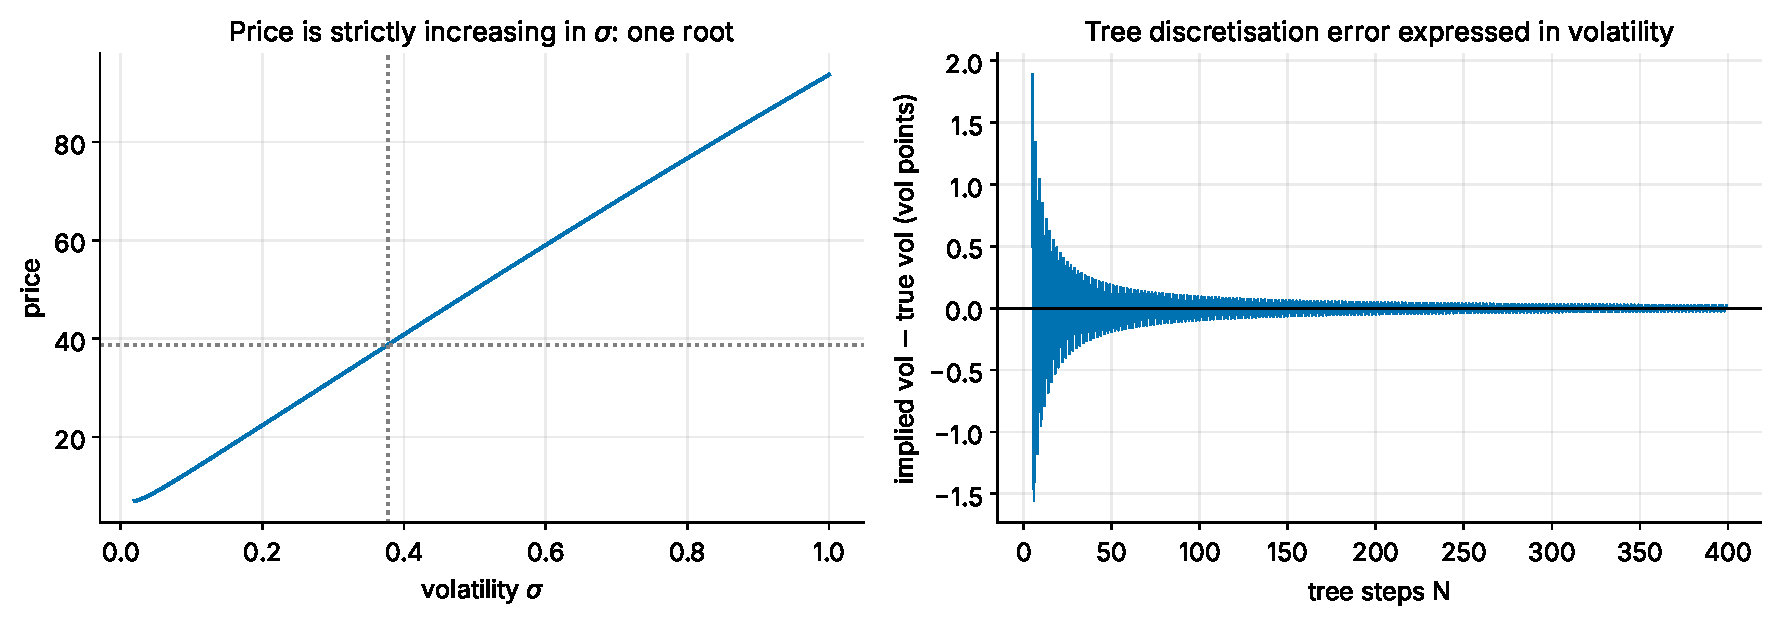
\includegraphics[width=\textwidth]{implied_vol.pdf}
\caption{Left: the call price is strictly increasing in $\sigma$. Right: implied volatility of the CRR price minus the true volatility, for $N=5,\dots,399$.\label{fig:iv}}
\end{figure}

\subsection{Discrete delta hedging}\label{sec:hedge}
% P24 | 4.9 Hedging | Result: delta hedging in discrete time
% guide: dev_notes/paragraph_guides/P24_result_delta_hedging_in_discrete_time.txt
The seller of the call receives the Black--Scholes price $C_0$, holds $\Delta_k=\Phi(d_1)$ shares at $n$ equally spaced dates and finances the position at rate $r$.
The discounted profit is
\begin{equation}\label{eq:hedgeerr}
 \varepsilon=C_0+\sum_{k=0}^{n-1}\Delta_k\big(e^{-rt_{k+1}}S_{t_{k+1}}-e^{-rt_k}S_{t_k}\big)-e^{-rT}(S_T-K)^+,
\end{equation}
which is zero in continuous time.
Table~\ref{tbl:hedgefreq} and Figure~\ref{fig:hedge} show that the standard deviation of $\varepsilon$ decays like $n^{-1/2}$, with a fitted slope of \HedgeSlope.
With daily rebalancing it is \$\HedgeSDdaily, which is \HedgeSDdailyPct\% of the premium, and with weekly rebalancing it is \$\HedgeSDweekly, or \HedgeSDweeklyPct\%.
The mean error is close to zero and the dispersion is the same, within simulation noise, when the stock is simulated with the real-world drift instead of the risk-neutral one.
The hedge therefore works whatever the drift, which is the practical content of the statement that $\mu$ does not enter the price.
The residual error is the sum of $n$ gamma-weighted surprises of the squared return, each of size proportional to $1/n$, which explains the square-root law.
Cutting the hedging risk in half therefore needs four times as many trades, and with transaction costs this is where hedging becomes a cost-benefit decision.


\begin{table}[h!]
\centering
\begin{tabular}{rcccc}
\toprule
rebalances $n$ & sd of hedging error (\$) & as \% of premium & mean error (\$) & sd under real-world drift \\
\midrule
4 & 14.187 & 36.6 & -0.099 & 14.692 \\
8 & 10.302 & 26.6 & +0.073 & 10.521 \\
16 & 7.391 & 19.1 & +0.027 & 7.303 \\
32 & 5.286 & 13.6 & +0.040 & 5.270 \\
52 & 4.152 & 10.7 & -0.061 & 4.194 \\
64 & 3.778 & 9.7 & +0.022 & 3.750 \\
126 & 2.653 & 6.8 & +0.028 & 2.711 \\
252 & 1.908 & 4.9 & -0.004 & 1.925 \\
\bottomrule
\end{tabular}

\caption{Standard deviation of the discounted hedging error of a short call against the number of rebalances $n$ (risk-neutral paths; last column with real-world drift $\mu=10\%$). Premium $\$\BSprice$.\label{tbl:hedgefreq}}
\end{table}

% P25 | 4.9 Hedging | Result: hedging with the wrong volatility
% guide: dev_notes/paragraph_guides/P25_result_hedging_with_the_wrong_volatility.txt
If the stock has realised volatility $\sigma_{real}$ and the hedge uses $\sigma_h$, the discounted profit of the seller is, to leading order,
\begin{equation}\label{eq:gammapnl}
 \varepsilon\approx\int_0^Te^{-rt}\,\tfrac12\,\Gamma_t S_t^2\,(\sigma_h^2-\sigma_{real}^2)\,dt,
\end{equation}
so the seller loses when the realised variance exceeds the variance used to price and hedge.
Table~\ref{tbl:hedgewrong} compares the simulated mean profit with the integral in Equation~\eqref{eq:gammapnl} evaluated along the same paths.
At a realised volatility of $55\%$ the simulation gives \$\WrongVolLoss\ and the formula gives \$\WrongVolTheory.
At realised volatilities of $25\%$ and $30\%$ the sign reverses and the seller gains by comparable amounts, so the profit is close to linear in the variance gap.
The size of the error is large compared with the discretisation error of Table~\ref{tbl:hedgefreq}: choosing the wrong volatility costs far more than trading weekly instead of daily.
Section~\ref{sec:misspec} repeats this experiment for the American put, where a wrong volatility also corrupts the exercise rule.


\begin{table}[h!]
\centering
\begin{tabular}{rccc}
\toprule
realised $\sigma$ & simulated mean P\&L & gamma formula & sd of P\&L \\
\midrule
25.0\% & +11.704 & +11.714 & 3.726 \\
30.0\% & +7.109 & +7.116 & 2.803 \\
37.7\% & -0.013 & +0.000 & 1.953 \\
45.0\% & -6.672 & -6.685 & 3.583 \\
55.0\% & -15.781 & -15.716 & 7.780 \\
\bottomrule
\end{tabular}

\caption{Hedging with the wrong volatility ($\sigma_h=\NvdaSigma\%$, daily rebalancing, $10^4$ paths): simulated mean profit of the seller against the gamma formula.\label{tbl:hedgewrong}}
\end{table}

\begin{figure}[h!]
\centering
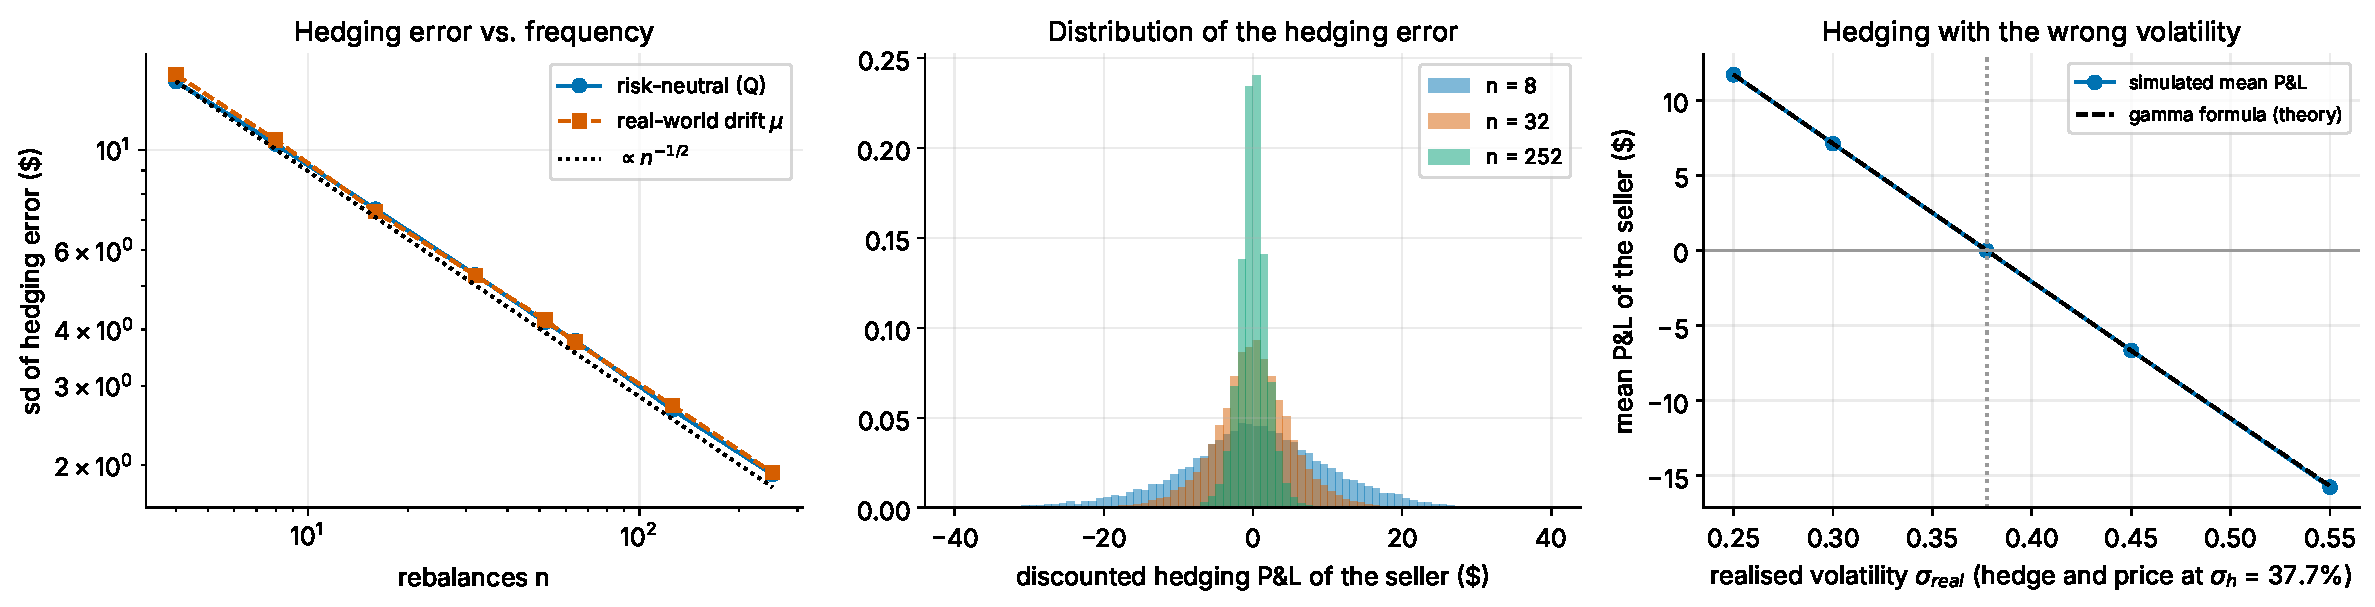
\includegraphics[width=\textwidth]{hedging_error.pdf}
\caption{Left: standard deviation of the hedging error against $n$. Middle: distribution of the error for three values of $n$. Right: mean profit when the realised volatility differs from the hedging volatility.\label{fig:hedge}}
\end{figure}

% P26 | 4 Part B summary | What Part B shows about the European call
% guide: dev_notes/paragraph_guides/P26_what_part_b_shows_about_the_european_call.txt
For a single European call on one stock, a Leisen--Reimer tree or a smoothed and extrapolated CRR tree is orders of magnitude more accurate than Monte Carlo for the same run time.
The work--precision comparison in Section~\ref{sec:compare} puts numbers on this.
Monte Carlo wins when the payoff depends on the whole path or on many underlyings, because its error rate does not depend on the dimension, while the cost of a lattice grows exponentially with it.
Variance reduction closes part of the gap: a control variate alone was worth a factor of \VRcv\ in variance here.
The three routes to the Greeks agree, so the choice among them is a matter of cost and variance, not of correctness.
The hedging error of a short call falls only like $n^{-1/2}$ with the number of rebalances, and an error of $10$ volatility points in the hedge volatility costs more than any reasonable change of frequency.
Early exercise needs a decision at every date based on the value of waiting, which the tree computes naturally and Monte Carlo can approximate only with a regression, as Part C shows.

\FloatBarrier

% ======================================================================================== 5
\section{Part C: the American put}\label{sec:C}

\subsection{Optimal stopping}\label{sec:C-stop}
% P27 | 5.1 Optimal stopping | The American put as an optimal stopping problem
% guide: dev_notes/paragraph_guides/P27_the_american_put_as_an_optimal_stopping_problem.txt
An American put may be exercised at any time $\tau\le T$ and then pays $(K-S_\tau)^+$.
The holder chooses $\tau$ using only the information available, a stopping time, so under $\mathbb Q$ the fair value is the optimal stopping problem
\begin{equation}\label{eq:V}
 V(t,x)=\sup_{\tau\in[t,T]}\mathbb E\Big[e^{-r(\tau-t)}(K-S_\tau)^+\,\Big|\,S_t=x\Big].
\end{equation}
Two bounds follow at once: $V(t,x)\ge(K-x)^+$, by exercising immediately, and $V(t,x)\ge V^{Eur}(t,x)$, by choosing $\tau=T$.
The American put is therefore never worth less than the European put or than its intrinsic value.
The state space splits into a continuation region $C=\{V>(K-x)^+\}$ and a stopping region $D=\{V=(K-x)^+\}$, which for a put has the form $\{x\le b(t)\}$.
The boundary $b(t)$ is a free boundary, because it is part of the unknown and has to be found together with $V$, and the optimal rule is $\tau^*=\inf\{t:S_t\le b(t)\}$.
Equivalently, the discounted value $e^{-rt}V(t,S_t)$ is the smallest $\mathbb Q$-supermartingale that dominates the discounted payoff, the Snell envelope, and both the tree and the PDE are discretisations of this principle.


\subsection{The variational PDE and hedging}\label{sec:C-vi}
% P28 | 5.1 Optimal stopping | The variational PDE
% guide: dev_notes/paragraph_guides/P28_the_variational_pde.txt
Consider first a European claim and let $g(t,S_t)=e^{-rt}P(t,S_t)$ be a martingale.
Assuming $g\in C^{1,2}$ and applying It\^o's formula with $dS=rS\,dt+\sigma S\,dW$ gives
\begin{equation}\label{eq:ito}
 d\big(e^{-rt}P\big)=e^{-rt}\big(\partial_tP+rx\,\partial_xP+\tfrac12\sigma^2x^2\partial_{xx}P-rP\big)\,dt+e^{-rt}\sigma x\,\partial_xP\,dW,
\end{equation}
and a martingale has zero drift, so $(\mathcal L-r)P=0$ with $P(T,x)=h(x)$, which is the Black--Scholes PDE.
For the American put the discounted value $e^{-rt}V$ is only a supermartingale, so the drift in Equation~\eqref{eq:ito} is non-positive everywhere.
It must also dominate the obstacle $(K-x)^+$, and it is a martingale while the holder waits optimally, so the drift vanishes in the continuation region.
Together these facts give the variational inequality, also called a linear complementarity problem:
\begin{equation}\label{eq:VI}
 (\mathcal L-r)V\le0,\quad V\ge(K-x)^+,\quad \big(V-(K-x)^+\big)(\mathcal L-r)V=0,\quad V(T,x)=(K-x)^+ .
\end{equation}
At every point either the obstacle binds or the PDE holds with equality, and in a single line the system reads $\min\{-(\mathcal L-r)V,\;V-(K-x)^+\}=0$.
In the continuation region $x>b(t)$ the PDE holds with equality, and in the stopping region $V=K-x$, where $(\mathcal L-r)(K-x)=-rx-r(K-x)=-rK$.
This is negative for $r>0$, so waiting loses money in the stopping region, which is exactly why the holder exercises there.


% P29 | 5.1 Optimal stopping | Smooth fit and hedging
% guide: dev_notes/paragraph_guides/P29_smooth_fit_and_hedging.txt
The boundary $b(t)$ is part of the unknown, and the condition that fixes it is smooth fit: $\partial_xV$ is continuous across the boundary, so $\partial_xV(t,b(t))=-1$.
Heuristically, if $\partial_xV$ jumped at the boundary, the stopping rule could be improved by moving the boundary slightly.
A numerical solver never has to impose smooth fit, because the maximum in the tree recursion, or the projection in a finite-difference scheme, solves the obstacle problem directly.
Because the market is complete, the second fundamental theorem of asset pricing implies that the claim exercised at $\tau^*$ can be replicated by holding $\Delta_t=\partial_xV(t,S_t)$ shares and the rest in the bond.
This is the delta hedge of the European option with the American value function: the formula is the same, the function is different, and $\Delta=-1$ in the stopping region because there $V=K-x$.
The replication is exact up to $\tau^*$, and if the holder exercises at any other time the seller is left with a surplus, so the hedge super-replicates every exercise date.
Section~\ref{sec:replication} checks this statement numerically in the tree.


\subsection{The perpetual put}\label{sec:perp}
% P30 | 5.2 Perpetual put | The perpetual put in closed form
% guide: dev_notes/paragraph_guides/P30_the_perpetual_put_in_closed_form.txt
If $T=\infty$ nothing depends on $t$, so the boundary is a constant $b(t)\equiv S^*$ and the system~\eqref{eq:VI} becomes an ODE,
\begin{equation}\label{eq:perp}
 \tfrac12\sigma^2x^2V''+rxV'-rV=0\ (x>S^*),\qquad V=K-x\ (x\le S^*),\qquad V\ge(K-x)^+,
\end{equation}
with $V$ and $V'$ continuous at $S^*$.
Trying $V=Ax^{-\beta}$ with $\beta>0$, so that $V\to0$ as $x\to\infty$, turns the ODE into $(\beta+1)\big(\tfrac12\sigma^2\beta-r\big)=0$, hence $\beta=2r/\sigma^2$.
In the notation $\kappa=r/\sigma^2$ and $\Delta=\sqrt{(\kappa-\frac12)^2+2\kappa}=\kappa+\frac12$ this reads $\beta=\kappa-\frac12+\Delta=2\kappa$.
Matching the value and the slope at $S^*$, that is $A(S^*)^{-\beta}=K-S^*$ and $-\beta A(S^*)^{-\beta-1}=-1$, determines both constants:
\begin{equation}\label{eq:Vinf}
 S^*=\frac{\beta K}{\beta+1},\qquad V_\infty(x)=\frac{K}{\beta+1}\Big(\frac{S^*}{x}\Big)^{\beta}\quad(x>S^*).
\end{equation}
A second derivation avoids smooth fit: exercising at the first time the price falls to a threshold $b$ is worth $V_b(x)=(K-b)(b/x)^\beta$, because $\mathbb E[e^{-r\tau_b}]=(b/x)^\beta$.
Maximising $(K-b)b^\beta$ over $b$ gives $b=\beta K/(\beta+1)=S^*$, so smooth fit is nothing but the first-order condition of the stopping problem.


\subsection{The CRR tree with early exercise}\label{sec:C-tree}
% P31 | 5.3 CRR tree for the American put | The tree with early exercise
% guide: dev_notes/paragraph_guides/P31_the_tree_with_early_exercise.txt
With $\Delta t=T/M_{bin}$, the CRR parameters of Section~\ref{sec:B} and $V_{M,i}=(K-S_{M,i})^+$, the American put is priced by
\begin{equation}\label{eq:crr}
 V_{j,i}=\max\Big\{(K-S_{j,i})^+,\;e^{-r\Delta t}\big(p\,V_{j+1,i+1}+(1-p)\,V_{j+1,i}\big)\Big\},
\end{equation}
where the first term is the value of exercising now and the second the value of waiting.
The exercise boundary $b(t_j)$ is the largest node at which exercising is strictly better than waiting, with a tolerance of $10^{-12}$ so that ties are resolved in favour of waiting.
The tolerance matters for $r=0$, where exercise and continuation coincide deep in the money, and because the nodes of a CRR tree alternate between two grids on odd and even layers the boundary is plotted on even layers only.
The hedge at node $(j,i)$ is the ratio $\Delta_{j,i}=\frac{V_{j+1,i+1}-V_{j+1,i}}{S_{j+1,i+1}-S_{j+1,i}}$ of the changes in option value and stock price over one step.
The optimal stopping time of a simulated path is the first date at which the path lies in the exercise region, and it is held to maturity if it never does.
The class \texttt{CRRTree} extends \texttt{CRRBinomialModel} of Section~\ref{sec:B}: it adds the American recursion, a vectorised simulation of paths and the stopping rule, and inherits the lattice.
The base class counts maturity in trading days, so the subclass passes \texttt{days=round(252*T)}, and each layer of the recursion is evaluated with array operations.


% P32 | 5.3 CRR tree for the American put | Why the tree solves the variational inequality
% guide: dev_notes/paragraph_guides/P32_why_the_tree_solves_the_variational_inequality.txt
We show that, in the continuation region, one step of the recursion reproduces the PDE as $\Delta t\to0$.
Write $y=\sigma\sqrt{\Delta t}$ so that $u=e^y$ and expand the value function at the two successor nodes.
A Taylor expansion to order $\Delta t$ gives the two successor values
\begin{align}
V(t+\Delta t,xu)&=V+V_t\Delta t+V_x\,x\big(\sigma\sqrt{\Delta t}+\tfrac12\sigma^2\Delta t\big)+\tfrac12V_{xx}x^2\sigma^2\Delta t+\dots\\
V(t+\Delta t,xd)&=V+V_t\Delta t+V_x\,x\big(-\sigma\sqrt{\Delta t}+\tfrac12\sigma^2\Delta t\big)+\tfrac12V_{xx}x^2\sigma^2\Delta t+\dots
\end{align}
From $pu+(1-p)d=e^{r\Delta t}$ one obtains $2p-1=\frac{(r-\frac12\sigma^2)\sqrt{\Delta t}}{\sigma}+o(\sqrt{\Delta t})$.
Hence the $\sqrt{\Delta t}$-terms contribute $(r-\tfrac12\sigma^2)x\,\Delta t\,V_x$, the $\tfrac12\sigma^2\Delta t\,xV_x$ terms complete this to $rxV_x\Delta t$, and $pV_u+(1-p)V_d=V+\big(V_t+rxV_x+\tfrac12\sigma^2x^2V_{xx}\big)\Delta t+o(\Delta t)$.
Multiplying by $e^{-r\Delta t}=1-r\Delta t+\dots$ and requiring the right-hand side of Equation~\eqref{eq:crr} to equal $V$ gives $(\mathcal L-r)V=0$ in the continuation region, while in the stopping region the maximum sets $V=K-x$.
Complementarity is therefore automatic, the tree is an explicit finite-difference scheme for the variational inequality~\eqref{eq:VI}, and both give the same price as $M_{bin}\to\infty$.


\subsection{Results: price, boundary and hedge}\label{sec:C-conv}
% P33 | 5.4 Results | Result: the perpetual put
% guide: dev_notes/paragraph_guides/P33_result_the_perpetual_put.txt
For the baseline $\kappa=0.5$, so $\beta=\PerpBeta$, $S^*=\PerpSstar$ and $V_\infty(10)=\PerpV$ (Figure~\ref{fig:Vinf}).
The perpetual put is worth $2.5$ at the money, more than three times the one-year American put of Section~\ref{sec:C-conv}.
A numerical check confirms that $V_\infty$ solves the system~\eqref{eq:perp}: the ODE residual is below \PerpResidual\ on $x>S^*$, the generator equals $-rK<0$ on $x<S^*$, the value is above the payoff everywhere and the slope on the right of $S^*$ is within $2\cdot10^{-4}$ of $-1$.
The value and the payoff coincide at $S^*$.
Since $\beta=2r/\sigma^2$ and $S^*/K=\beta/(\beta+1)$, a higher interest rate raises $\beta$ and moves $S^*/K$ towards one, so one exercises earlier because the strike earns interest.
A higher volatility lowers $\beta$ and $S^*/K$, because the option to wait is worth more; Figure~\ref{fig:beta} shows both dependences.
The level $S^*$ is the price below which waiting no longer pays for its cost, and the perpetual put is the limit of the long-dated puts tested in Section~\ref{sec:C-long}.


\begin{figure}[h!]
\begin{minipage}{0.48\textwidth}\centering
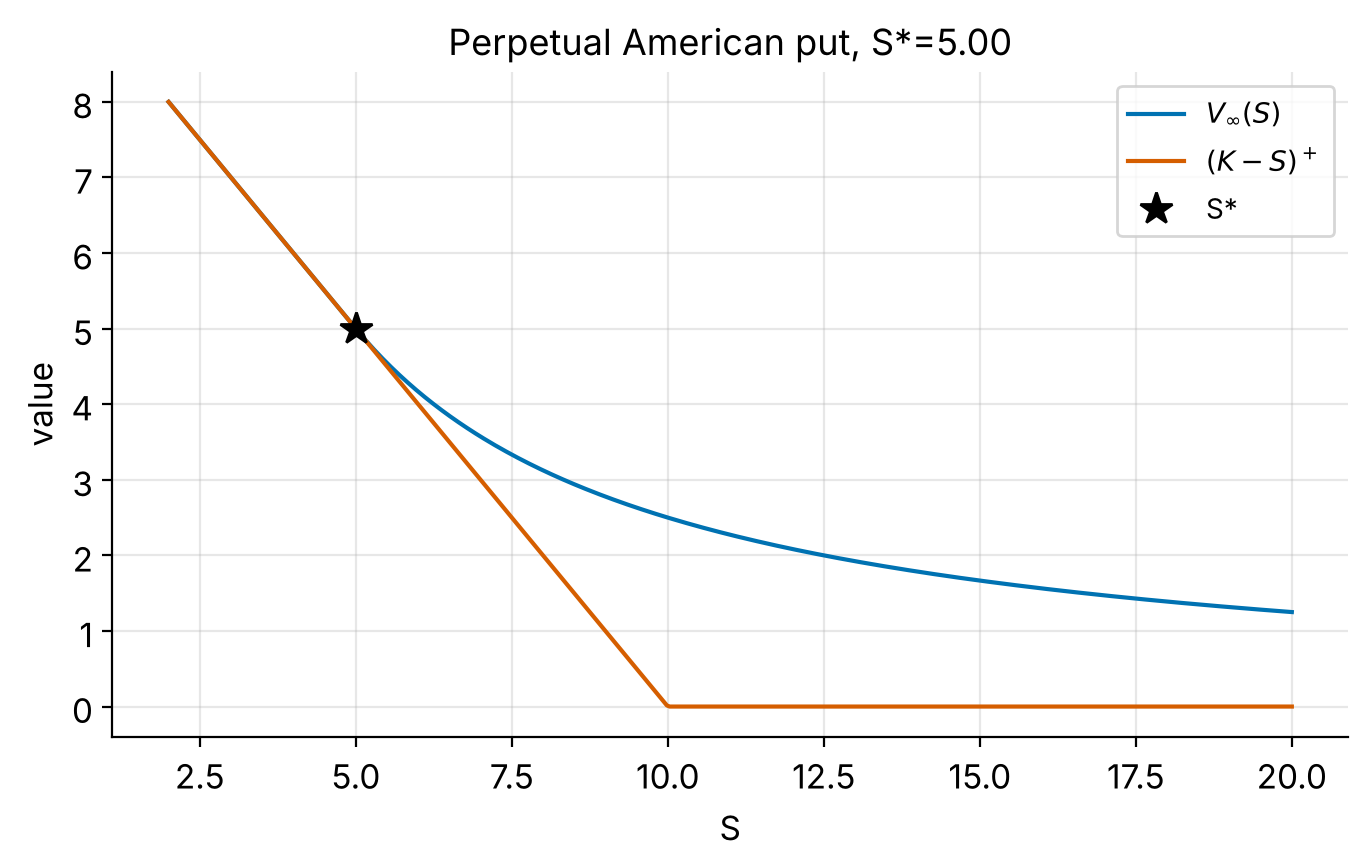
\includegraphics[width=\textwidth]{1c_Vinf.png}
\caption{$V_\infty(S)$ and $S^*=5$.\label{fig:Vinf}}
\end{minipage}\hfill
\begin{minipage}{0.48\textwidth}\centering
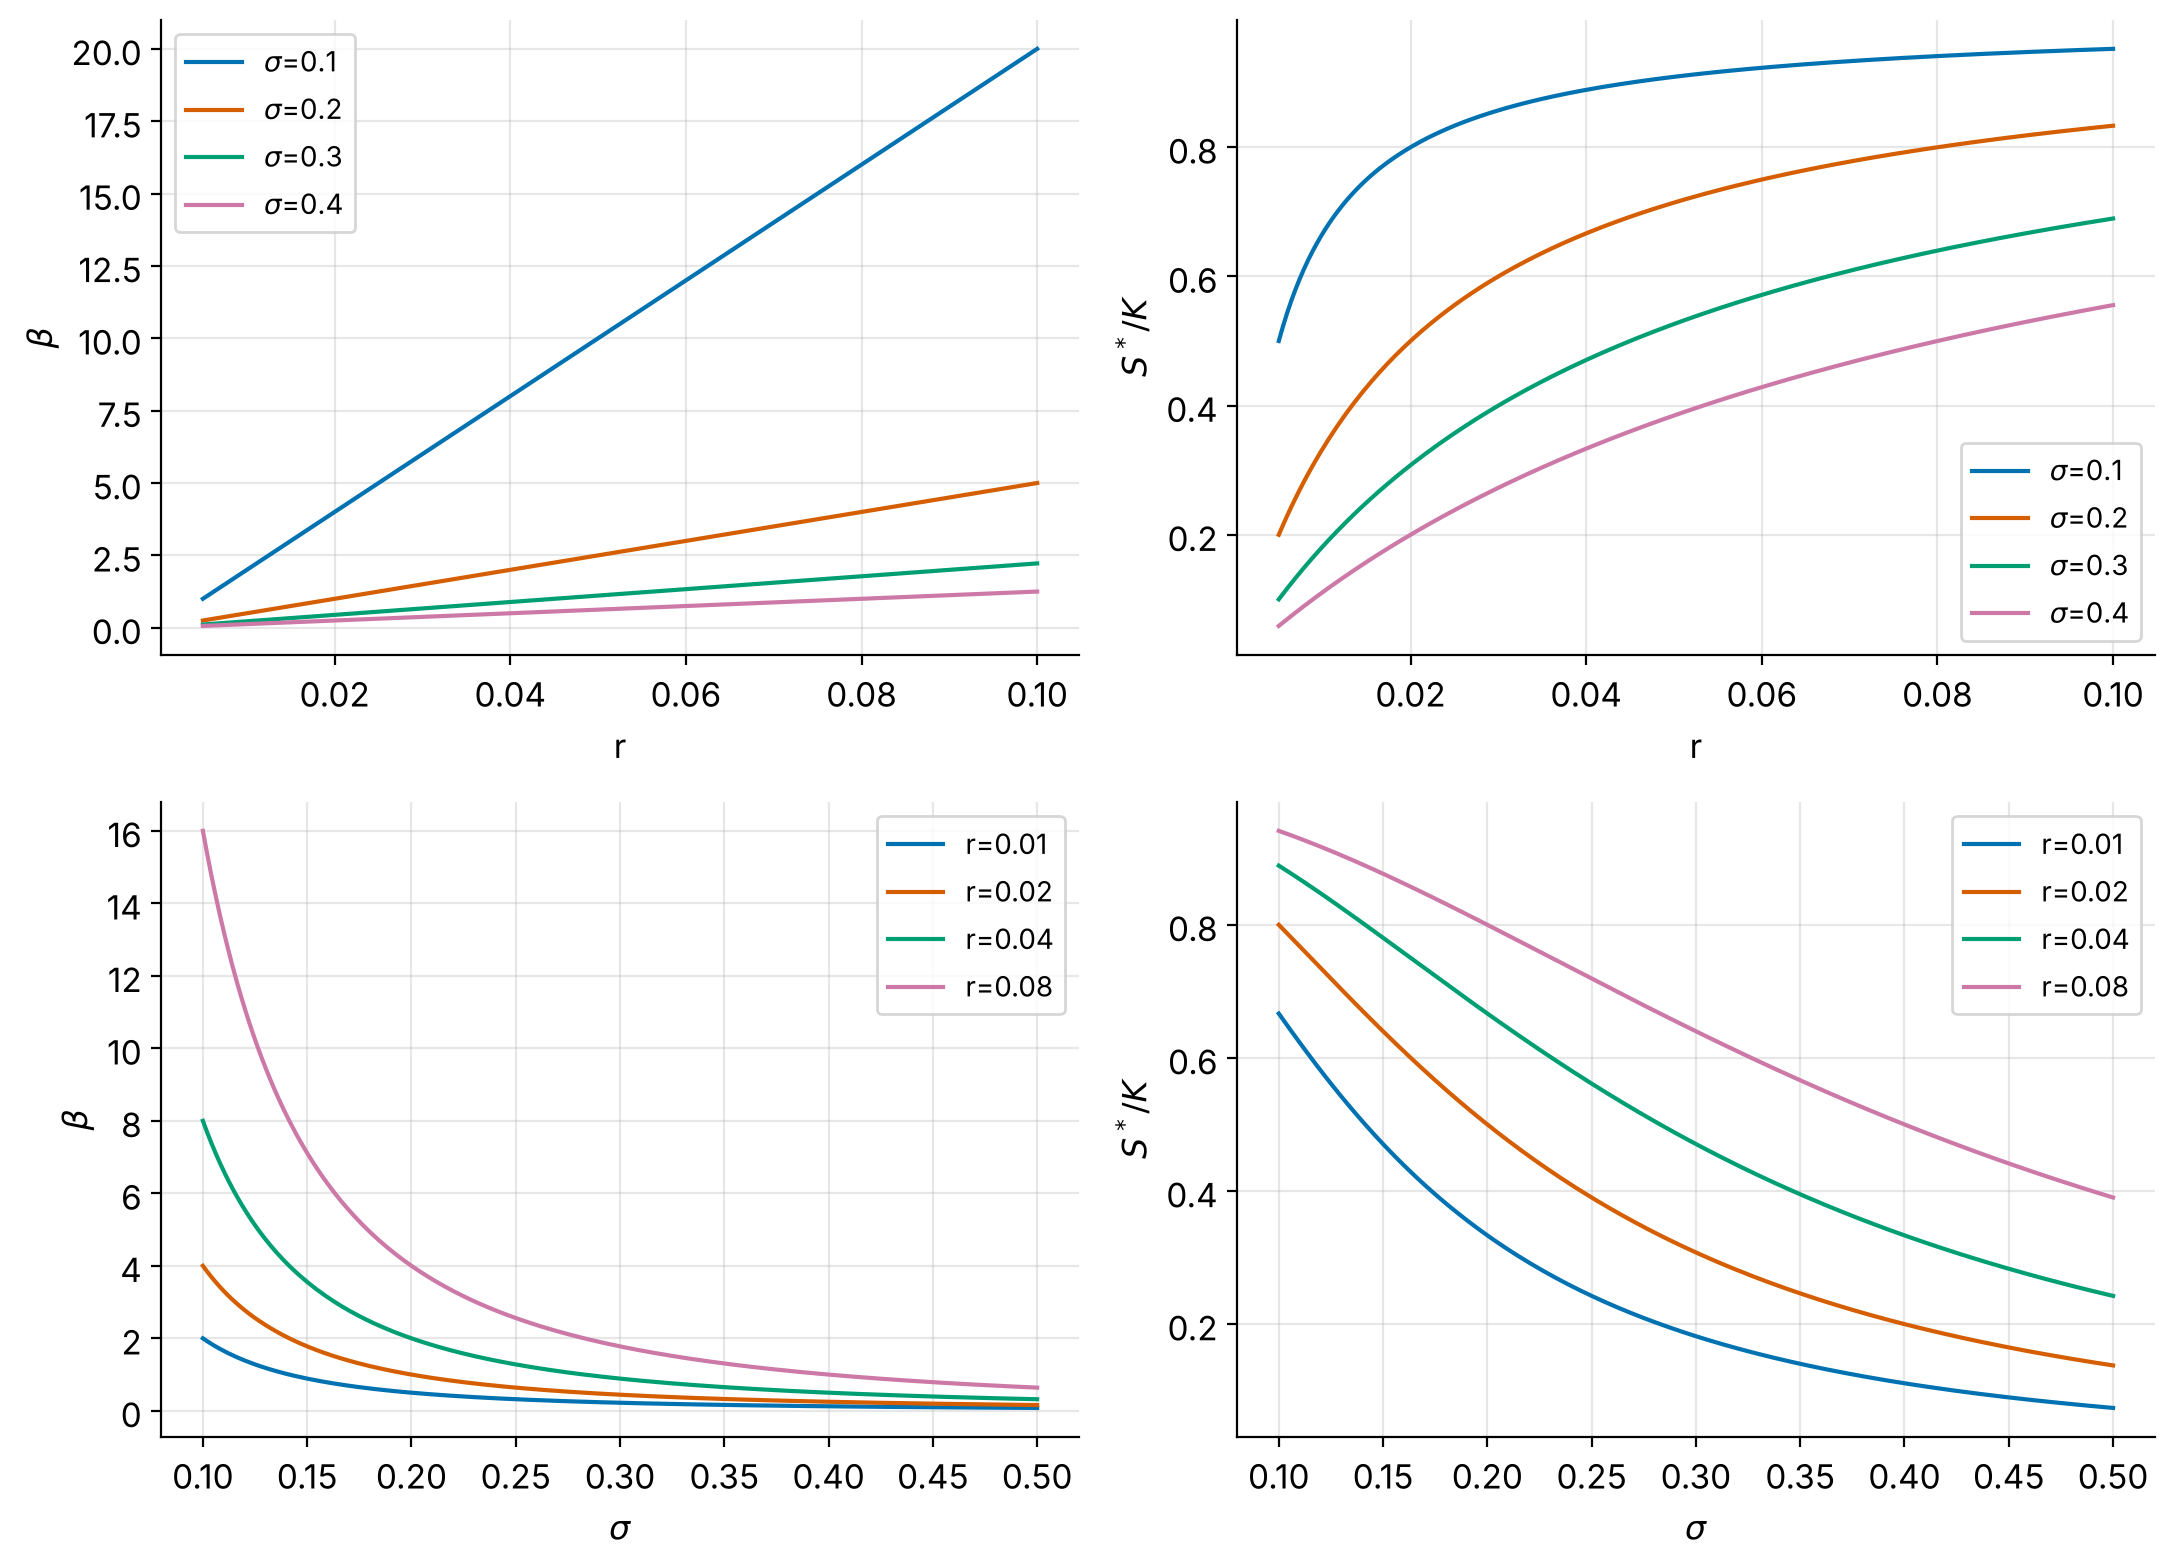
\includegraphics[width=\textwidth]{1c_beta_Sstar.png}
\caption{$\beta$ and $S^*/K$ against $r$ and $\sigma$.\label{fig:beta}}
\end{minipage}
\end{figure}

% P34 | 5.4 Results | Result: a two-step tree worked by hand
% guide: dev_notes/paragraph_guides/P34_result_a_two_step_tree_worked_by_hand.txt
With $M=2$ steps, $\Delta t=0.5$, $u=e^{0.2\sqrt{0.5}}=1.15191$, $d=0.86812$, $p=0.50012$ and $e^{-r\Delta t}=0.99005$.
The stock takes the values $10$, then $8.6812$ or $11.5191$, then $7.5364$, $10$ or $13.2690$.
At the lower node of the first layer, where $S=8.68$, exercising pays $1.3188$ while waiting is worth $0.99005\,(0.50012\cdot0+0.49988\cdot2.4636)=1.2193$.
The holder therefore exercises early at this node, which is the first place where the American recursion differs from the European one.
This lifts the price from the European value of \TwoStepEu\ to the American value of \TwoStepAm.
The hedge ratio at the root is $\Delta_{0,0}=\frac{0-1.3188}{11.5191-8.6812}=\TwoStepDelta$, so the replicating portfolio of the put is short about half a share, and the seller of the put hedges by holding that much.


% P35 | 5.4 Results | Result: convergence in the number of steps and the exercise boundary
% guide: dev_notes/paragraph_guides/P35_result_convergence_in_the_number_of_steps_and_th.txt
Table~\ref{tbl:amconv} shows that the tree price increases from $0.7088$ at $M_{bin}=50$ to \AmVeight\ at $M_{bin}=800$ and \AmV\ at $M_{bin}=1600$.
The successive changes halve each time $M_{bin}$ doubles, so the ratio in the fourth column stays close to $2$.
A ratio of two is the signature of first-order convergence, $O(1/M_{bin})$, as for the European tree.
Extrapolating, the limit is close to $0.7111$, a value confirmed by independent methods in Section~\ref{sec:validators}.
The exercise boundary $b(t;1)$ in Figure~\ref{fig:b} rises from about \AmBearly\ near $t=0$ to the strike at maturity, and the curves for the six step counts lie on top of each other.
At $t=0.5$ it equals \AmBhalf\ for the finest tree, and the column of Table~\ref{tbl:amconv} varies only by about one lattice spacing between step counts.
With six months left the holder exercises once the stock has fallen about a fifth below the strike, and close to maturity the boundary approaches $K$.
This shape reflects the trade-off behind the problem: waiting forgoes interest on the strike, which is worth more than the remaining optionality when the option is deep in the money.


\begin{table}[h!]
\centering
\begin{tabular}{rcccc}
\toprule
$M_{bin}$ & $V^{bin}(0,S_0)$ & change & ratio & $b(0.5;1)$ \\
\midrule
50 & 0.70877 & -- & -- & 7.97 \\
100 & 0.70995 & 0.00117 & -- & 7.87 \\
200 & 0.71051 & 0.00057 & 2.07 & 7.75 \\
400 & 0.71080 & 0.00029 & 1.97 & 7.87 \\
800 & 0.71094 & 0.00014 & 2.04 & 7.86 \\
1600 & 0.71101 & 0.00007 & 2.00 & 7.87 \\
\bottomrule
\end{tabular}

\caption{CRR price convergence of the American put, $T=1$: change, ratio of successive changes and boundary at $t=0.5$.\label{tbl:amconv}}
\end{table}

\begin{figure}[h!]
\begin{minipage}{0.48\textwidth}\centering
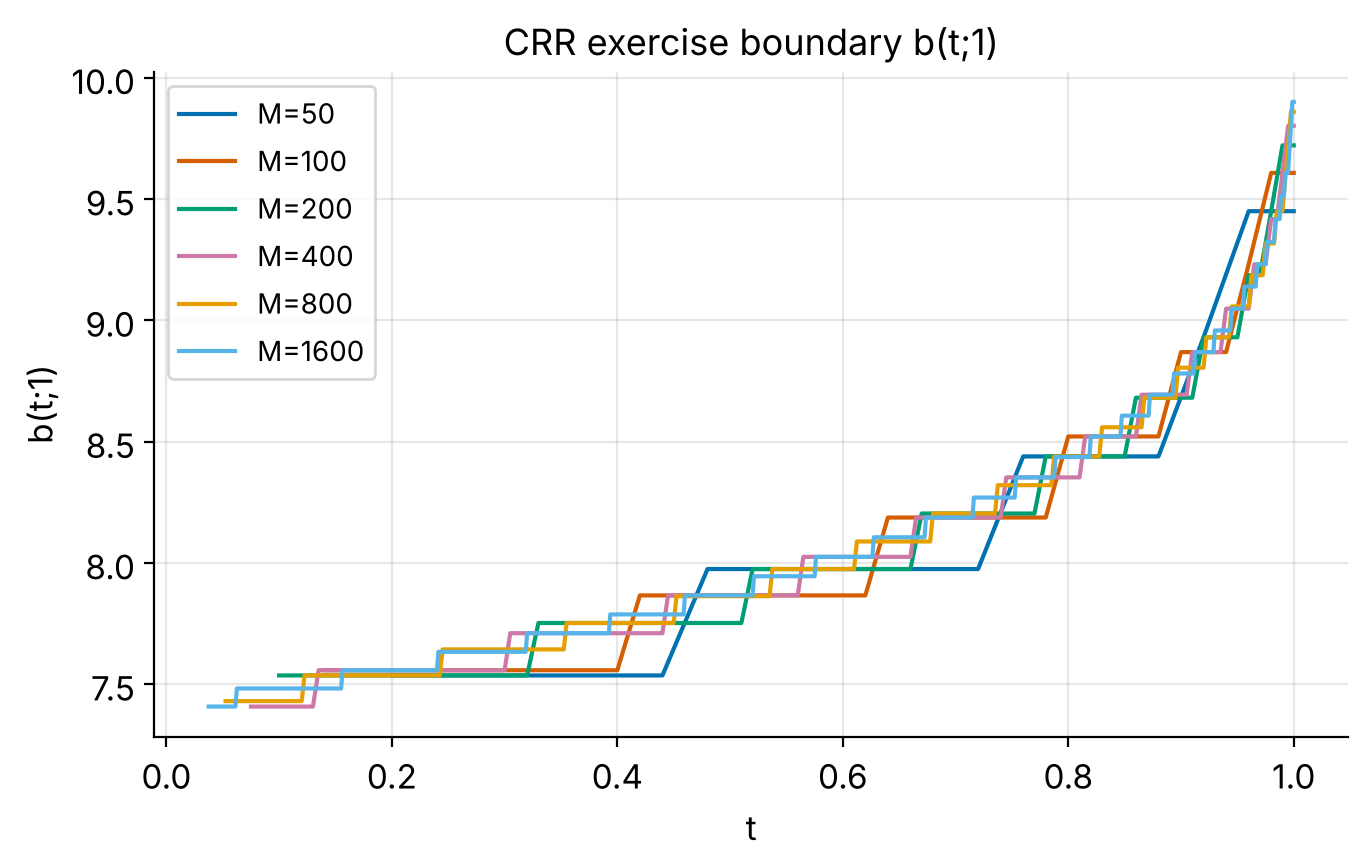
\includegraphics[width=\textwidth]{2b_boundary.png}
\caption{Exercise boundary $b(t;1)$.\label{fig:b}}
\end{minipage}\hfill
\begin{minipage}{0.48\textwidth}\centering
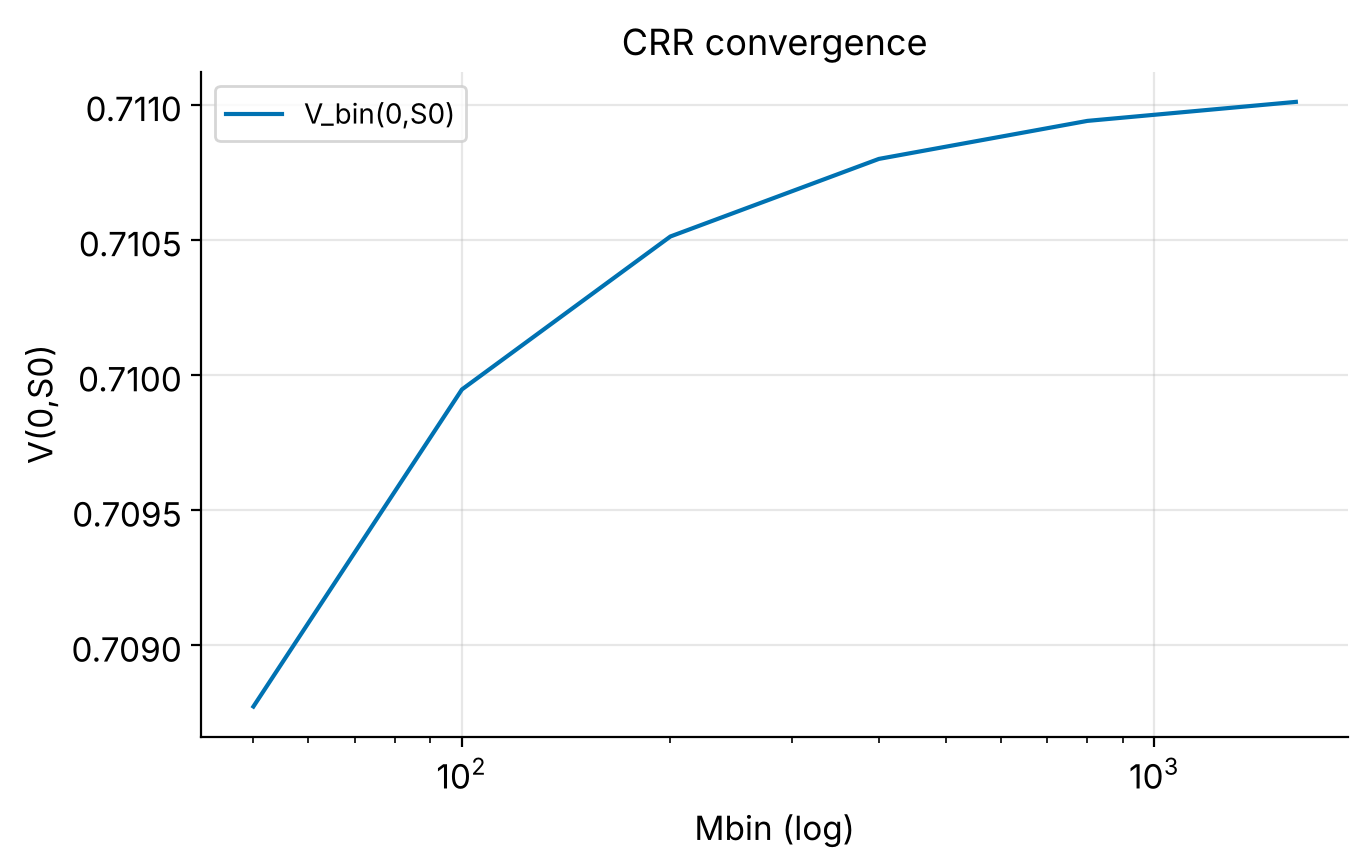
\includegraphics[width=\textwidth]{2b_convergence.png}
\caption{Convergence of $V^{bin}(0,S_0)$.\label{fig:conv}}
\end{minipage}
\end{figure}

% P36 | 5.4 Results | Result: two sample paths and the delta hedge
% guide: dev_notes/paragraph_guides/P36_result_two_sample_paths_and_the_delta_hedge.txt
Path 1 in Figure~\ref{fig:paths} first enters the exercise region at $t=\PathOneTau$ and is stopped there, whereas Path 2 never enters it and is held to maturity.
Both paths were selected from a random search with fixed seed to illustrate the two cases.
Along Path 1 the hedge ratio starts at \DeltaStart\ and moves to \DeltaPathOneEnd\ as the path approaches the boundary, so the replicating portfolio ends up short almost one full share, and the seller of the put holds almost one full share (Figure~\ref{fig:delta}).
This is the smooth-fit condition seen from the hedger's side: the slope of the value function tends to $-1$ at the boundary.
Along Path 2 the stock moves away from the strike, the put loses value, and the hedge ratio returns towards $0$ near maturity.
The hedge for an option that ends out of the money is therefore unwound without ever reaching the exercise region.
A European put has no such plateau: its hedge ratio stays strictly above $-1$ at every spot and every date.


\begin{figure}[h!]
\begin{minipage}{0.48\textwidth}\centering
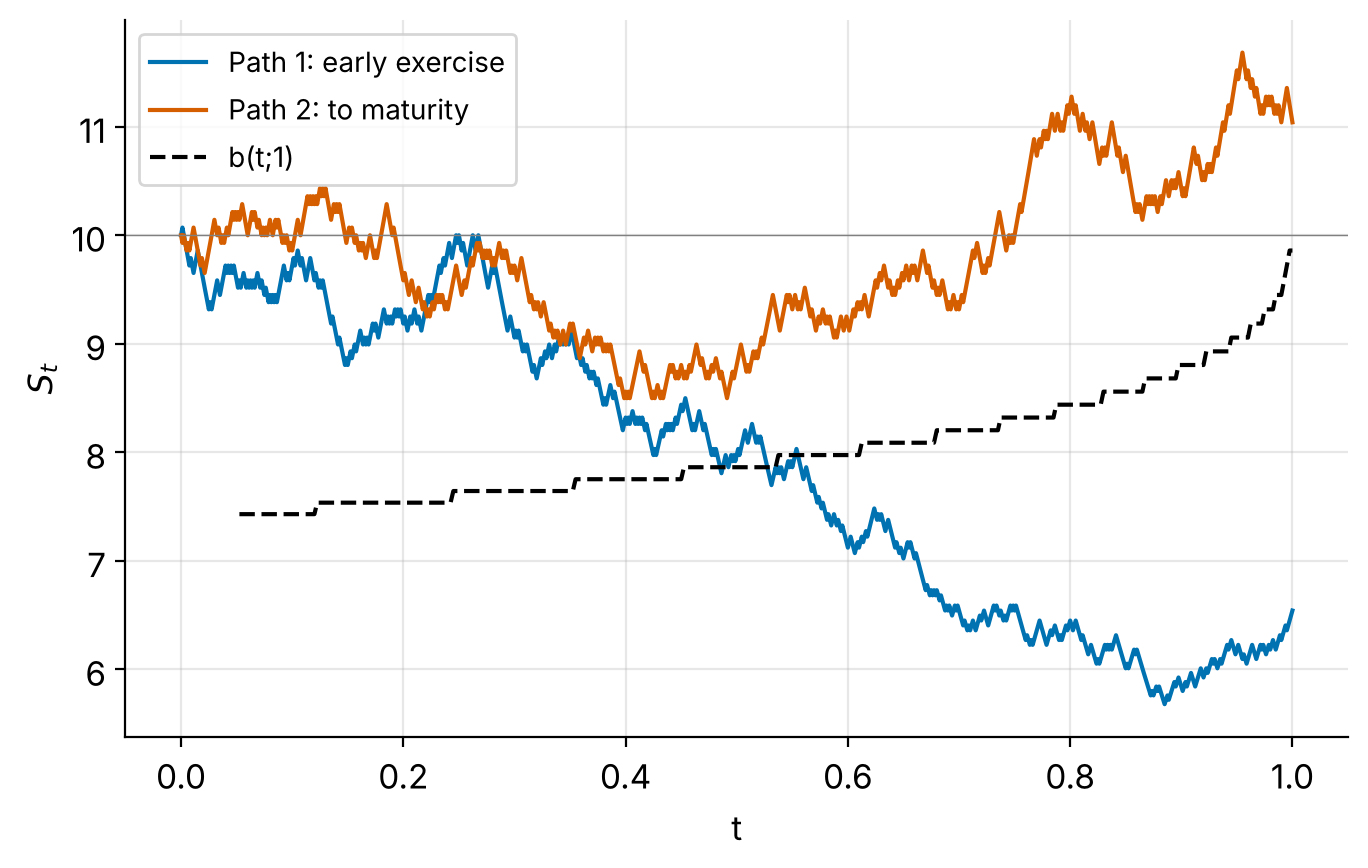
\includegraphics[width=\textwidth]{2c_paths.png}
\caption{Two simulated paths and $b(t;1)$.\label{fig:paths}}
\end{minipage}\hfill
\begin{minipage}{0.48\textwidth}\centering
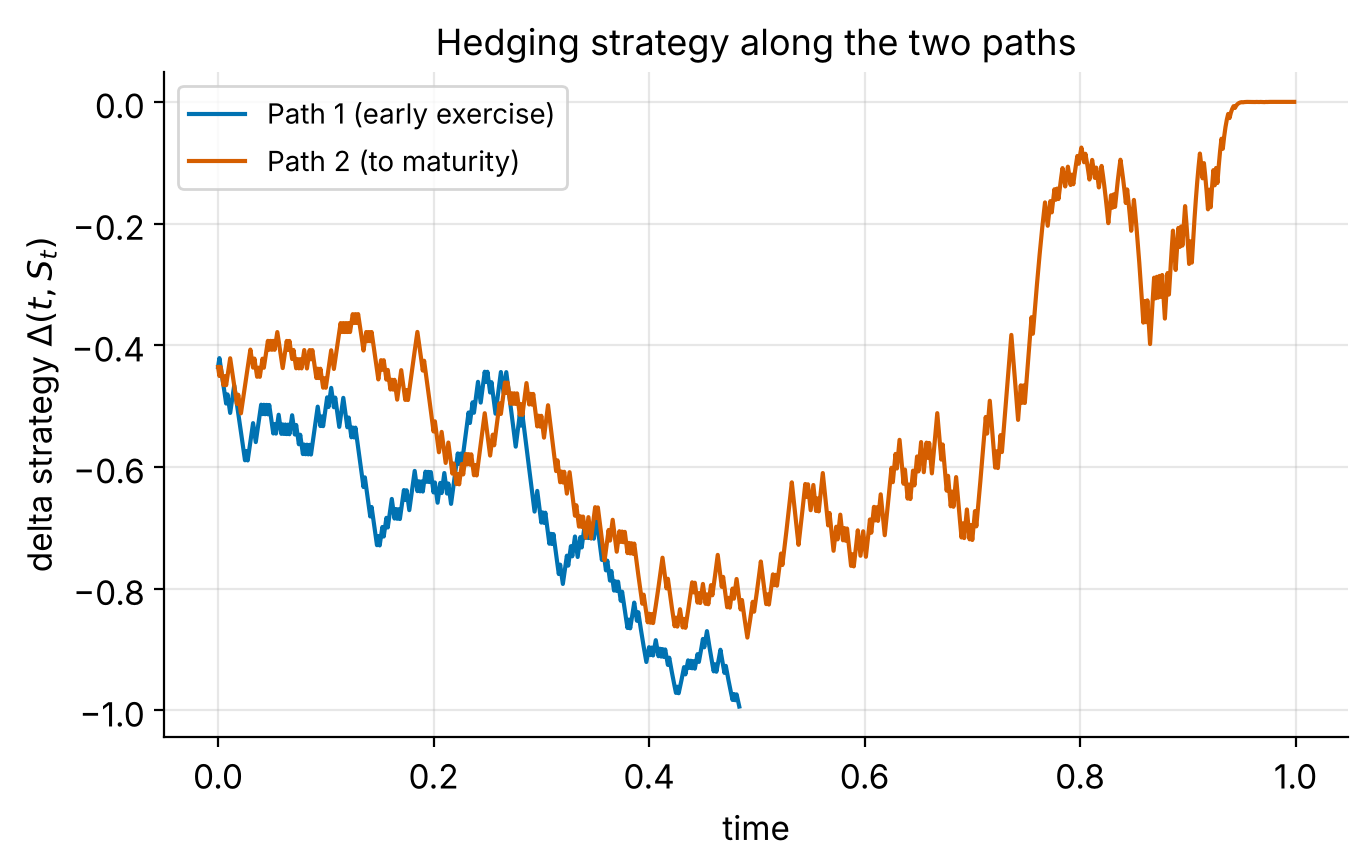
\includegraphics[width=\textwidth]{2d_delta.png}
\caption{Hedging strategy $\Delta(t,S_t)$ along both paths.\label{fig:delta}}
\end{minipage}
\end{figure}

% P37 | 5.4 Results | Result: dependence on volatility and interest rate
% guide: dev_notes/paragraph_guides/P37_result_dependence_on_volatility_and_interest_rat.txt
Higher volatility lowers the boundary: at $t=0.5$ and $r=2\%$ it equals \BhalfLow, \BhalfMid\ and \BhalfHigh\ for $\sigma=10\%$, $20\%$ and $30\%$.
The option to wait is worth more when the stock is more volatile, so the holder is willing to wait longer, and the price rises with $\sigma$ (Table~\ref{tbl:amsr}).
A higher interest rate raises the boundary, from \BhalfMid\ to \BhalfRhigh\ when $r$ goes from $2\%$ to $4\%$ at $\sigma=20\%$, because the strike earns interest once the option is exercised.
The price falls with $r$ for the same reason that a put loses value when interest rates rise.
For $r=0$ the boundary is empty in Table~\ref{tbl:amsr} because waiting never costs anything, so the American put equals the European put.
Exercising early would give up optionality and gain no interest.
The hedge ratio at the start, $\Delta(0,S_0)$, lies between \DeltaRangeLo\ and \DeltaRangeHi\ and depends only mildly on $(\sigma,r)$.
Higher volatility flattens $\Delta(t,\cdot)$ as a function of spot, and for $r>0$ the plateau at $-1$ starts at the boundary, which is higher for larger $r$ and smaller $\sigma$ (Figure~\ref{fig:eh}).


\begin{table}[h!]
\centering
\begin{tabular}{cccccc}
\toprule
$\sigma$ & $r$ & $V(0,S_0)$ & $b(0.5)$ & $b(0.9)$ & $\Delta(0,S_0)$ \\
\midrule
0.1 & 0 & 0.3987 & -- & -- & -0.480 \\
0.1 & 0.02 & 0.3224 & 9.06 & 9.45 & -0.436 \\
0.1 & 0.04 & 0.2665 & 9.25 & 9.52 & -0.409 \\
0.2 & 0 & 0.7963 & -- & -- & -0.460 \\
0.2 & 0.02 & 0.7109 & 7.86 & 8.80 & -0.436 \\
0.2 & 0.04 & 0.6403 & 8.20 & 8.93 & -0.418 \\
0.3 & 0 & 1.1920 & -- & -- & -0.440 \\
0.3 & 0.02 & 1.1011 & 6.68 & 8.09 & -0.424 \\
0.3 & 0.04 & 1.0227 & 7.27 & 8.26 & -0.411 \\
\bottomrule
\end{tabular}

\caption{Price, boundary and delta for $M_{bin}=800$, $T=1$. A dash means that the tree never exercises early.\label{tbl:amsr}}
\end{table}

\begin{figure}[h!]
\centering
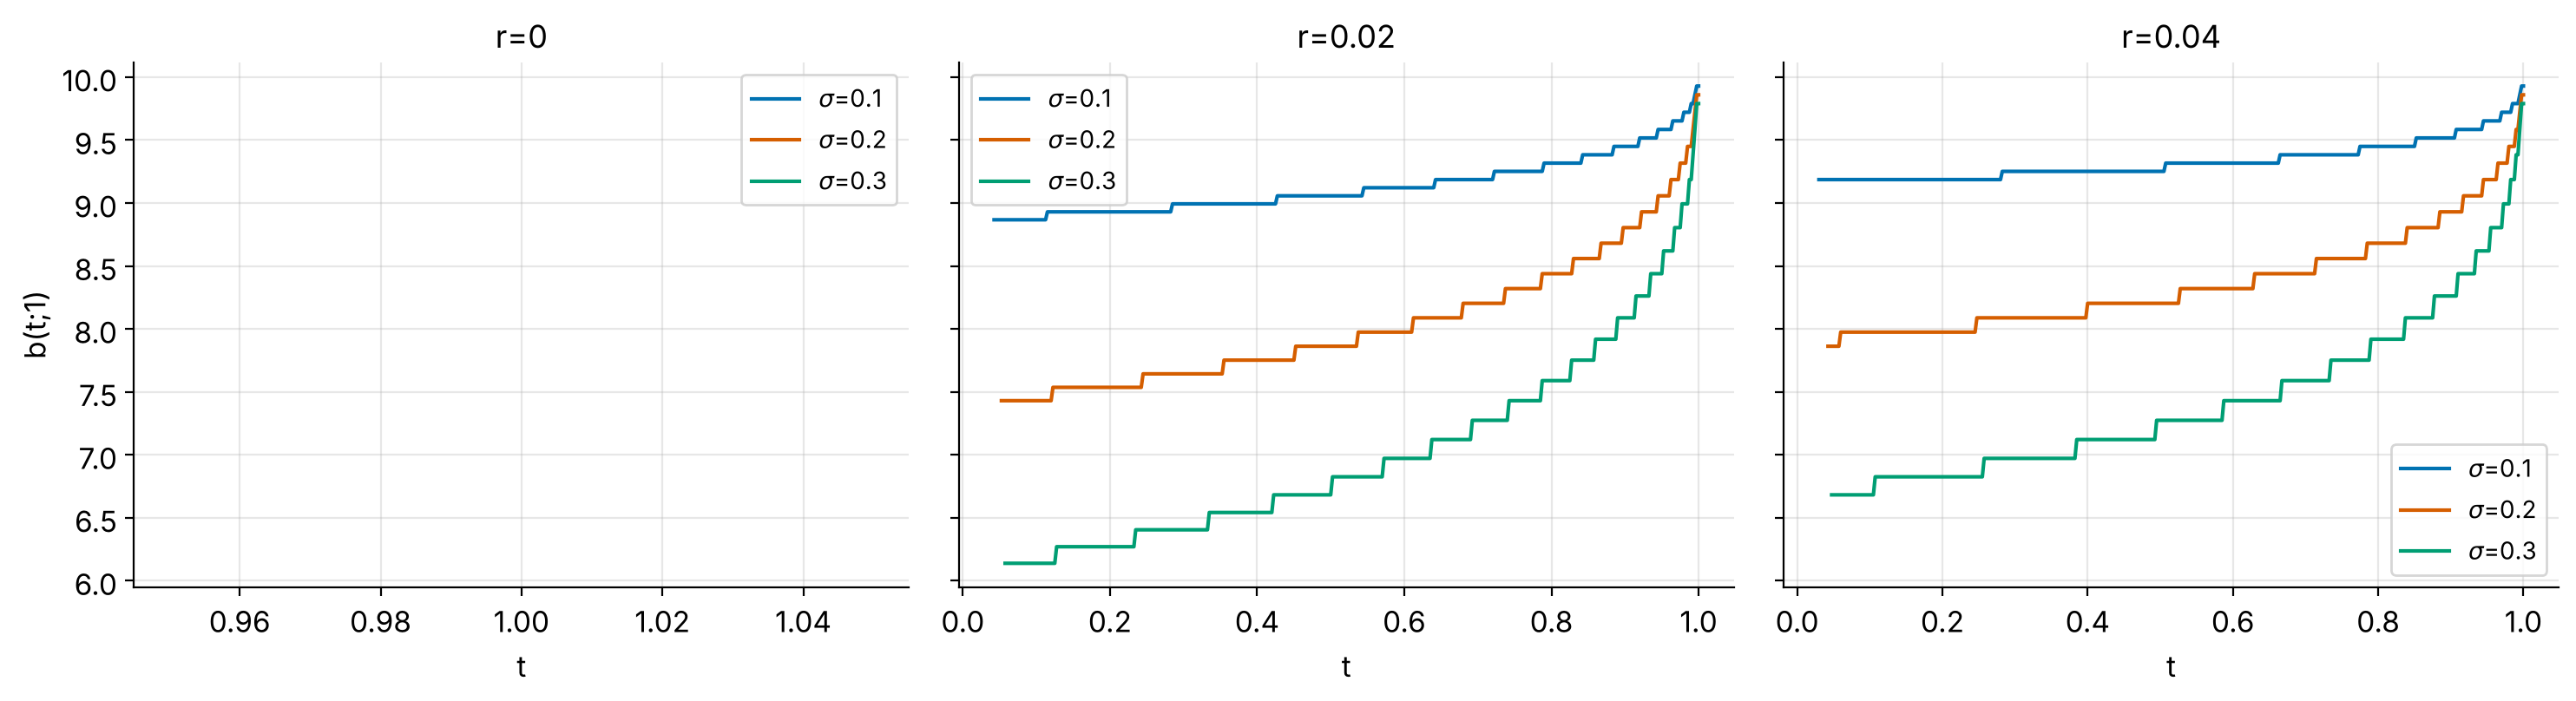
\includegraphics[width=\textwidth]{2e_boundary.png}
\caption{$b(t;1)$ for each $(\sigma,r)$.\label{fig:eb}}
\end{figure}

\begin{figure}[h!]
\centering
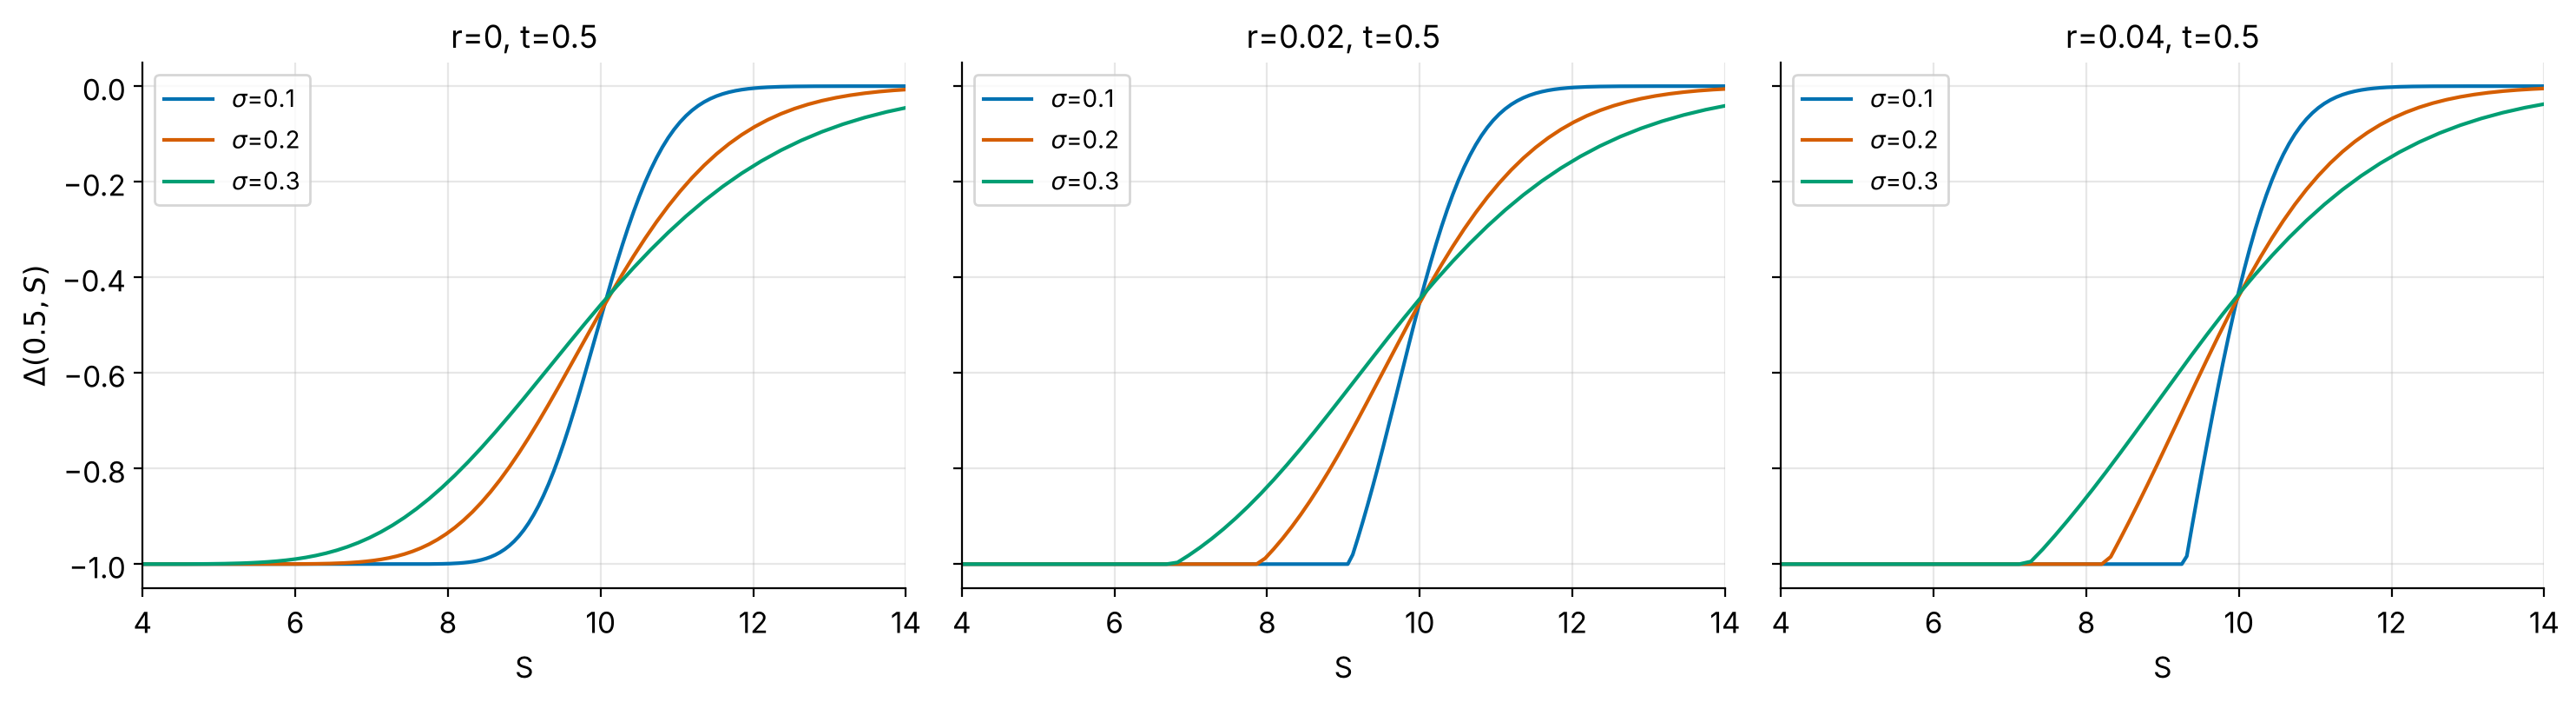
\includegraphics[width=\textwidth]{2e_hedging.png}
\caption{$\Delta(0.5,S)$ for each $(\sigma,r)$.\label{fig:eh}}
\end{figure}
\FloatBarrier

\subsection{Long maturities and the perpetual limit}\label{sec:C-long}
% P38 | 5.4 Results | Result: long maturities, as first computed
% guide: dev_notes/paragraph_guides/P38_result_long_maturities_as_first_computed.txt
With $M_{bin}=800$ steps for every maturity, the price $V(0,S_0)$ increases with $T$ towards the perpetual value of $2.5$: it is $1.72$ at $T=10$, $2.06$ at $T=20$, $2.38$ at $T=50$ and $2.47$ at $T=100$.
The curves $V(0,x)$ in Figure~\ref{fig:fVx} approach $V_\infty(x)$ for all $x$.
The boundary at date zero decreases from $5.8$ at $T=10$ to $5.1$ at $T=100$, towards $S^*=5$.
Plotted against the time to maturity $T-t$, the curves $b(t;T)$ for different $T$ coincide and flatten at $S^*$ (Figure~\ref{fig:fb}).
The row for $T=1000$ breaks the pattern: it gives $b(0;1000)=5.5$, above the value $5.1$ at $T=100$, and a price that has stopped improving.
An option that is almost perpetual cannot have a boundary that moves away from $S^*$, so the row must be a numerical artefact.
The artefact is the lattice: with $M_{bin}=800$ and $T=1000$ the step is $\Delta t=1.25$ and $u=1.25$, far too coarse to resolve a boundary near $5$, and the next paragraph repeats the experiment with a finer lattice.


\begin{table}[h!]
\centering
\begin{tabular}{rccc}
\toprule
$T$ & $V^{bin}(0,S_0)$ & $b(0;T)$ & $|V^{bin}-V_\infty|$ \\
\midrule
10 & 1.7207 & 5.8 & 0.7793 \\
20 & 2.0601 & 5.4 & 0.4399 \\
50 & 2.3766 & 5.2 & 0.1234 \\
100 & 2.4746 & 5.1 & 0.0254 \\
1000 & 2.4847 & 5.5 & 0.0153 \\
$\infty$ & 2.5000 & 5.0 & 0 \\
\bottomrule
\end{tabular}

\caption{Long maturities with $M_{bin}=800$ for every $T$ (first computation). The row $T=1000$ is a lattice artefact.\label{tbl:amlongcoarse}}
\end{table}

\begin{figure}[h!]
\begin{minipage}{0.32\textwidth}\centering
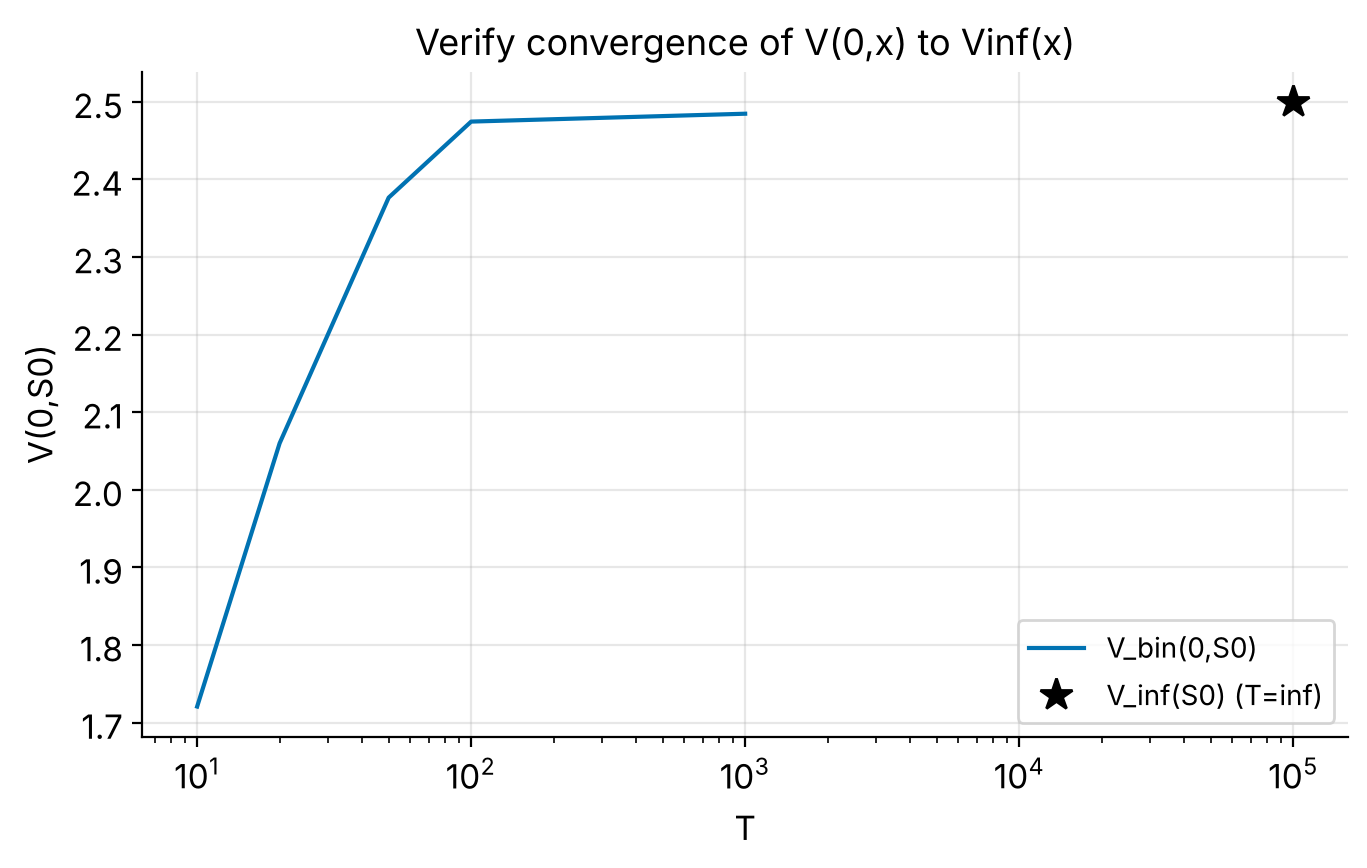
\includegraphics[width=\textwidth]{2f_V0_vs_T.png}
\caption{$V(0,S_0)$ against $T$.\label{fig:fV}}
\end{minipage}\hfill
\begin{minipage}{0.32\textwidth}\centering
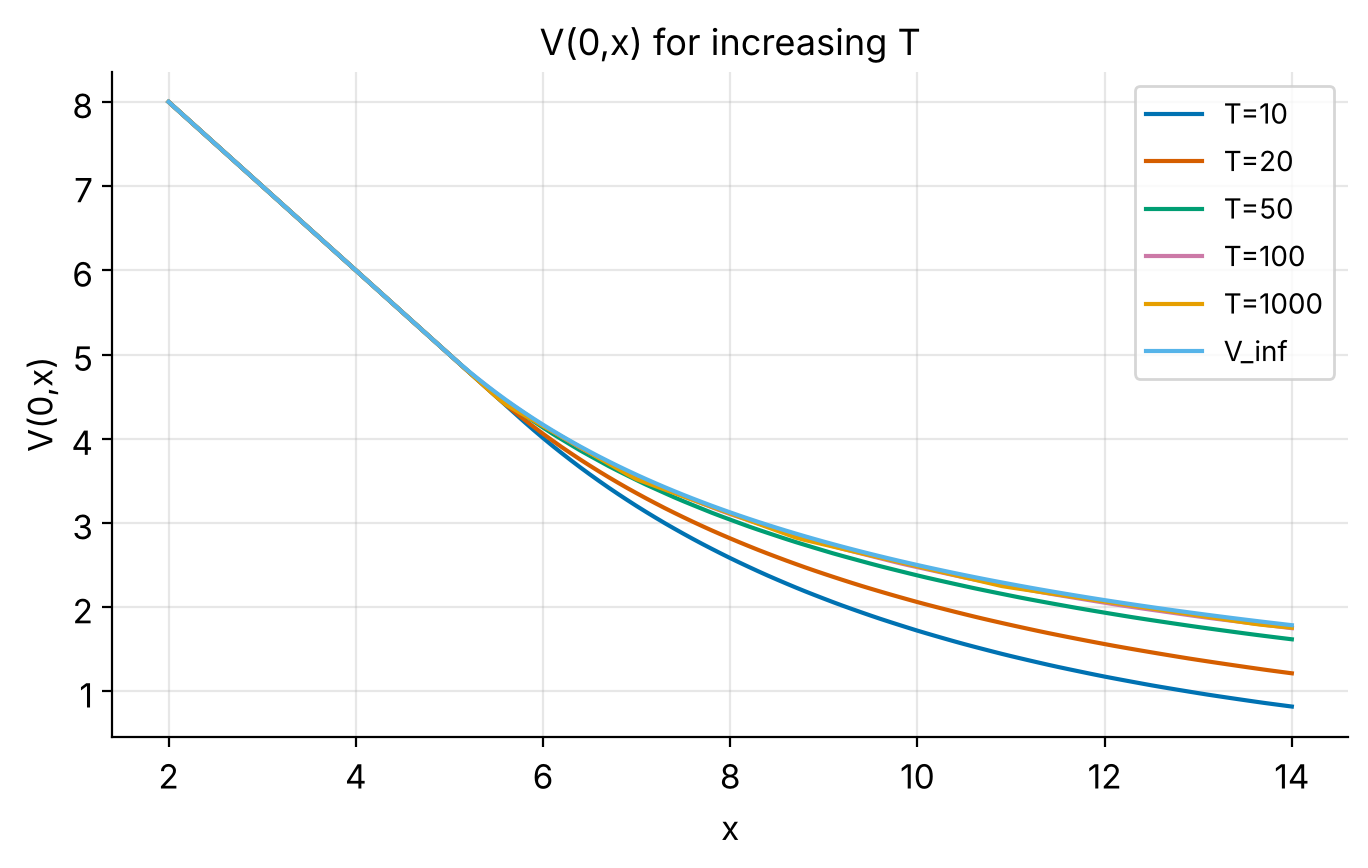
\includegraphics[width=\textwidth]{2f_Vx.png}
\caption{$V(0,x)$ against $V_\infty(x)$.\label{fig:fVx}}
\end{minipage}\hfill
\begin{minipage}{0.32\textwidth}\centering
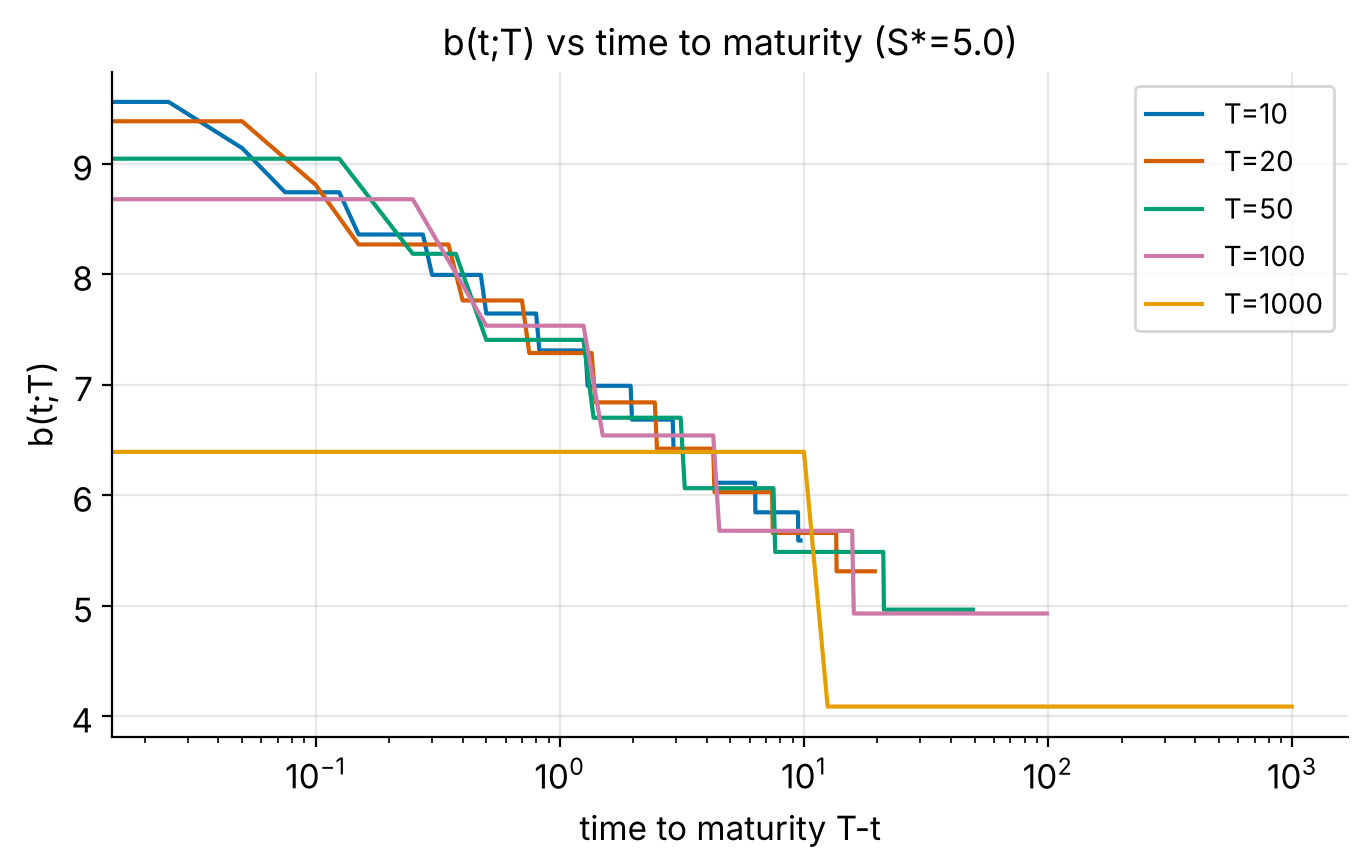
\includegraphics[width=\textwidth]{2f_boundary.png}
\caption{$b(t;T)$ against $T-t$.\label{fig:fb}}
\end{minipage}
\end{figure}

% P39 | 5.4 Results | Result: long maturities with a refined lattice
% guide: dev_notes/paragraph_guides/P39_result_long_maturities_with_a_refined_lattice.txt
Table~\ref{tbl:amlongfine} uses $M_{bin}=\max(800,8T)$ steps, so that $\Delta t\le0.125$, and finds the boundary at date zero by bisection on the decision at the root, which determines $b(0;T)$ to the accuracy of the bisection instead of to a grid of step $0.1$.
The price and the boundary now increase and decrease monotonically with $T$ up to $T=200$.
For $T=500$ and $T=1000$ the rows coincide, with $V=\LongVthousand$ and $b=\LongBthousand$, so the gap of \LongGapThousand\ to the perpetual value is no longer a maturity effect: it is a lattice effect.
At $T=1000$ the effect of maturity is of order $e^{-40}$.
Table~\ref{tbl:amlonglattice} refines the lattice at $T=500$: the gap to $2.5$ falls from \LatVgapCoarse\ to \LatVgap\ and the boundary comes down from \LatBcoarse\ to \LatBfine\ as $\Delta t$ goes from $0.25$ to $0.03$.
The price gap is not monotone in $M_{bin}$ (it oscillates with the position of the nodes relative to $S^*$), whereas the boundary error decreases steadily.
After subtracting the lattice floor of \LongFloor, the distance $V_\infty(S_0)-V(0,S_0)$ decays roughly exponentially in $T$, with a fitted rate of \LongDecay\ per year between $T=5$ and $T=100$ (Figure~\ref{fig:longT}).
This rate is an empirical fit, not a derived constant, and it applies to this parameter set only.


\begin{table}[h!]
\centering
\begin{tabular}{rrrcccc}
\toprule
$T$ & $M_{bin}$ & $\Delta t$ & $V^{bin}(0,S_0)$ & $b(0;T)$ & $V_\infty-V$ & $b-S^*$ \\
\midrule
2 & 800 & 0.003 & 0.9569 & 6.933 & 1.5431 & 1.933 \\
5 & 800 & 0.006 & 1.3676 & 6.262 & 1.1324 & 1.262 \\
10 & 800 & 0.013 & 1.7207 & 5.812 & 0.7793 & 0.812 \\
20 & 800 & 0.025 & 2.0601 & 5.466 & 0.4399 & 0.466 \\
50 & 800 & 0.062 & 2.3766 & 5.223 & 0.1234 & 0.223 \\
100 & 800 & 0.125 & 2.4746 & 5.196 & 0.0254 & 0.196 \\
200 & 1600 & 0.125 & 2.4966 & 5.180 & 0.0034 & 0.180 \\
500 & 4000 & 0.125 & 2.4980 & 5.179 & 0.0020 & 0.179 \\
1000 & 8000 & 0.125 & 2.4980 & 5.179 & 0.0020 & 0.179 \\
\bottomrule
\end{tabular}

\caption{Long maturities with a refined lattice ($M_{bin}=\max(800,8T)$) and the date-0 boundary found by bisection.\label{tbl:amlongfine}}
\end{table}

\begin{table}[h!]
\centering
\begin{tabular}{rccccc}
\toprule
$M_{bin}$ & $\Delta t$ & $V^{bin}(0,S_0)$ & $V_\infty-V$ & $b(0;T)$ & $b-S^*$ \\
\midrule
2000 & 0.2500 & 2.49697 & 0.00303 & 5.255 & 0.255 \\
4000 & 0.1250 & 2.49805 & 0.00195 & 5.179 & 0.179 \\
8000 & 0.0625 & 2.49915 & 0.00085 & 5.126 & 0.126 \\
16000 & 0.0312 & 2.49915 & 0.00085 & 5.089 & 0.089 \\
\bottomrule
\end{tabular}

\caption{Lattice refinement at $T=500$: the remaining gap to the perpetual values $V_\infty=2.5$ and $S^*=5$ is a lattice effect.\label{tbl:amlonglattice}}
\end{table}

\begin{figure}[h!]
\centering
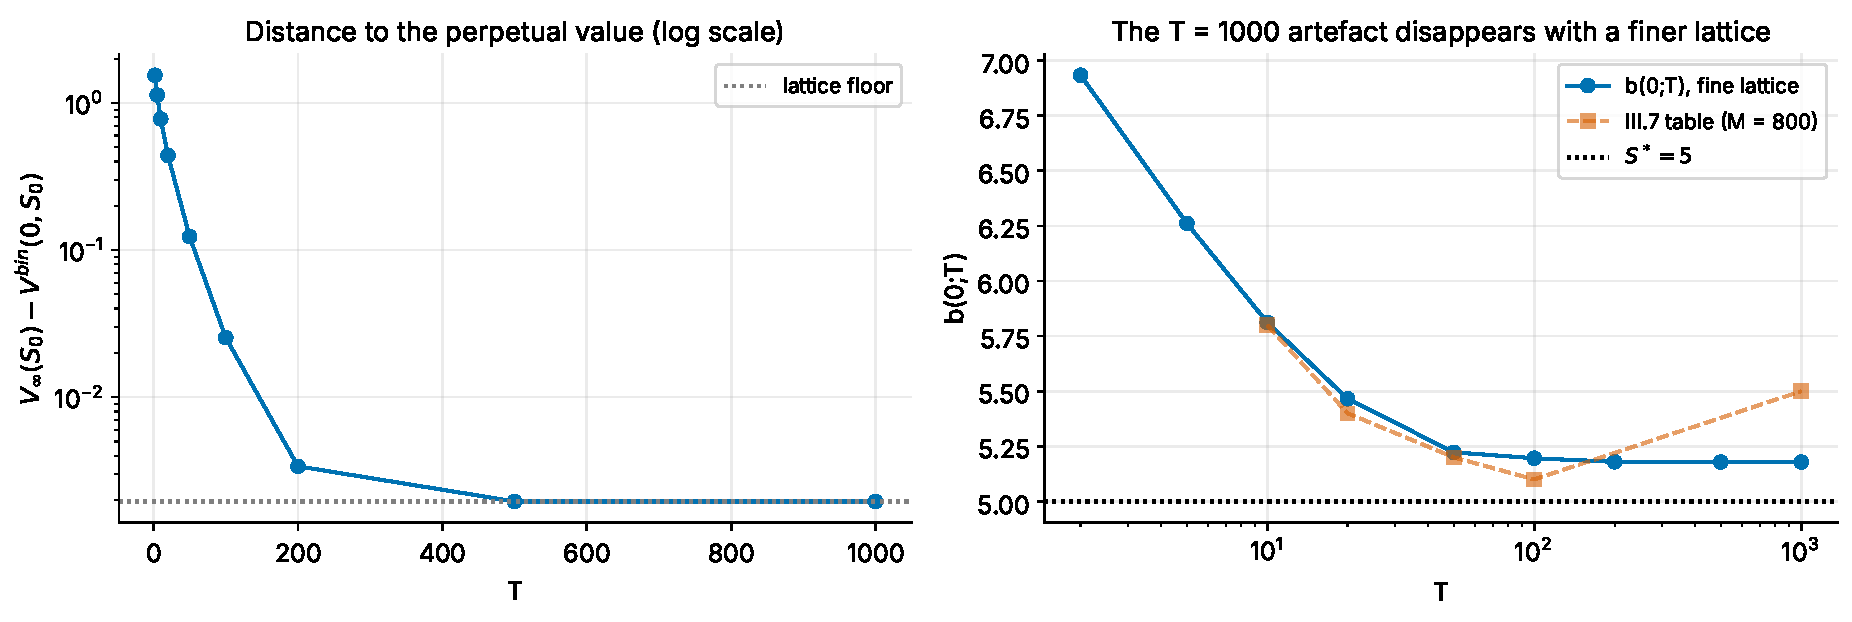
\includegraphics[width=\textwidth]{long_T_refined.pdf}
\caption{Left: distance to the perpetual value against $T$ (log scale), with the lattice floor. Right: $b(0;T)$ with the refined and the original lattice.\label{fig:longT}}
\end{figure}
\FloatBarrier

\subsection{Replication in the tree}\label{sec:replication}
% P40 | 5.5 Replication check | Result: the replication property in the tree
% guide: dev_notes/paragraph_guides/P40_result_the_replication_property_in_the_tree.txt
We simulate $200$ paths of the baseline tree with $800$ steps and, at every date before exercise, compare the value of the replicating portfolio one step later with the option value at the node that was reached.
The portfolio holds $\Delta_{j,i}$ shares and $B=V_{j,i}-\Delta_{j,i}S_{j,i}$ in the bond.
The largest discrepancy over all hedge dates on all paths is \ReplError, which is rounding error.
Replication is therefore exact in the tree up to the optimal exercise time.
Inside the exercise region the identity fails by construction, because the holder is paid $K-S$, which exceeds the continuation value that the hedge replicates.
The excess is the seller's surplus when the holder exercises, and at the boundary nodes we sampled it is tiny, of the order of $0.0002$ in price units.


\subsection{Independent validators: finite differences, regression Monte Carlo, approximation}\label{sec:validators}
% P41 | 5.6 Independent validators | Result: a finite-difference solver for the variational inequality
% guide: dev_notes/paragraph_guides/P41_result_a_finite_difference_solver_for_the_variat.txt
We solve the variational inequality~\eqref{eq:VI} on a uniform grid in $\ln x$ with Crank--Nicolson time stepping, started by four implicit half steps to smooth the kink of the payoff.
The obstacle is enforced by the penalty method, which iterates on the set of nodes where the value is at the payoff, and the exercise boundary is read from that set.
As a sanity check, the same code without the obstacle reproduces the Black--Scholes European put with an error of \PdeEuErr.
This tests the grid, the boundary conditions and the time stepping separately from the obstacle.
Table~\ref{tbl:pde} shows that the PDE price converges to \PdeV, against \TreeRichV\ for the Richardson-extrapolated tree, a difference of \PdeTreeDiff.
The PDE converges faster than the tree and its finest grid takes about a second.
Figure~\ref{fig:pdetree} overlays the exercise boundaries of the two methods, and they differ by at most \BoundGap\ for $t<0.97$.
This is smaller than the spacing of the tree's nodes near the strike, so the two boundaries agree within the resolution of the tree.


\begin{table}[h!]
\centering
\begin{tabular}{cccrr}
\toprule
grid points & time steps & $V(0,S_0)$ & error vs tree (Richardson) & CPU (s) \\
\midrule
201 & 50 & 0.710224 & -8.6e-04 & 0.02 \\
401 & 100 & 0.710826 & -2.5e-04 & 0.06 \\
801 & 200 & 0.711001 & -8.0e-05 & 0.14 \\
1601 & 400 & 0.711054 & -2.7e-05 & 0.43 \\
3201 & 800 & 0.711071 & -9.5e-06 & 1.49 \\
\bottomrule
\end{tabular}

\caption{Crank--Nicolson with penalty for the American put: grid refinement against the Richardson-extrapolated tree.\label{tbl:pde}}
\end{table}

\begin{figure}[h!]
\centering
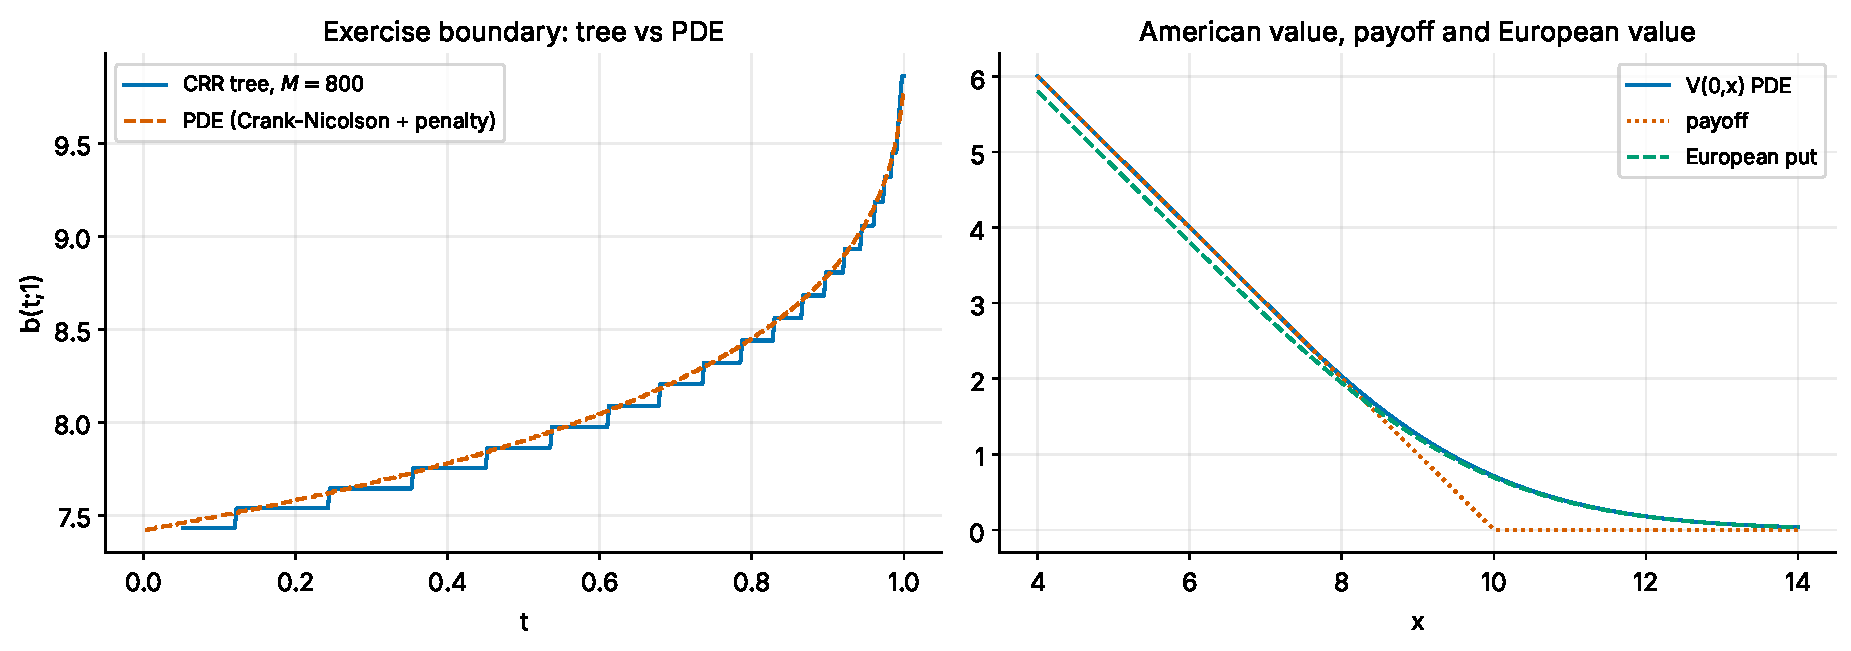
\includegraphics[width=\textwidth]{pde_vs_tree.pdf}
\caption{Left: exercise boundary from the tree ($M=800$) and from the PDE solver. Right: value, payoff and European value from the PDE solver.\label{fig:pdetree}}
\end{figure}

% P42 | 5.6 Independent validators | Result: least-squares Monte Carlo and the quasi-analytic approximation
% guide: dev_notes/paragraph_guides/P42_result_least_squares_monte_carlo_and_the_quasi_a.txt
Least-squares Monte Carlo works backward on simulated paths: at each exercise date it regresses the discounted future cash flow on a polynomial of the spot, using only in-the-money paths, and exercises when the payoff exceeds the fitted continuation value.
The estimate is biased low, because the regression policy is not the optimal one, and it approaches the Bermudan value as the basis grows.
With $50$ exercise dates and $2\cdot10^5$ paths the estimate is \LSMfifty\ with standard error \LSMfiftySE, against \BermFifty\ for a Bermudan tree on the same dates.
The difference is within one standard error, as it is for the other date counts in Table~\ref{tbl:lsm}.
The last column of Table~\ref{tbl:lsm} shows that the gap between the American and the Bermudan value halves as the number of exercise dates doubles.
Restricting exercise to fifty dates therefore costs about $0.0006$ in value, which is below the standard error of the regression estimate.
The Barone--Adesi--Whaley approximation, which approximates the early-exercise premium by a power of the spot, gives \BAWV\ at the baseline, an error of \BAWerr, and a critical price of \BAWSc\ against the tree boundary of about \AmBearly\ at the start.
Table~\ref{tbl:baw} shows that its absolute error grows with the maturity and reaches about one cent for the three-year put, which is why it serves for quick estimates and not for final prices.


\begin{table}[h!]
\centering
\begin{tabular}{ccccc}
\toprule
exercise dates & LSM (s.e.) & Bermudan tree & LSM $-$ Bermudan & American $-$ Bermudan \\
\midrule
10 & 0.7110 (0.0019) & 0.7085 & +0.0024 & +0.0026 \\
25 & 0.7092 (0.0019) & 0.7100 & -0.0008 & +0.0011 \\
50 & 0.7095 (0.0018) & 0.7105 & -0.0010 & +0.0006 \\
100 & 0.7106 (0.0018) & 0.7108 & -0.0002 & +0.0003 \\
\bottomrule
\end{tabular}

\caption{Longstaff--Schwartz ($2\cdot10^5$ paths) against a Bermudan tree with the same exercise dates.\label{tbl:lsm}}
\end{table}

\begin{table}[h!]
\centering
\begin{tabular}{ccccrc}
\toprule
$S_0$ & $T$ & European (BS) & American (tree) & BAW & BAW $-$ tree \\
\midrule
8 & 0.25 & 1.9547 & 2.0000 & 2.0000 & +0.0000 \\
10 & 0.25 & 0.3733 & 0.3768 & 0.3761 & -0.0007 \\
12 & 0.25 & 0.0129 & 0.0130 & 0.0131 & +0.0002 \\
8 & 1 & 1.9447 & 2.0323 & 2.0248 & -0.0075 \\
10 & 1 & 0.6936 & 0.7111 & 0.7100 & -0.0011 \\
12 & 1 & 0.1762 & 0.1791 & 0.1807 & +0.0016 \\
8 & 3 & 2.0351 & 2.2123 & 2.2019 & -0.0103 \\
10 & 3 & 1.0637 & 1.1277 & 1.1298 & +0.0021 \\
12 & 3 & 0.5222 & 0.5458 & 0.5532 & +0.0074 \\
\bottomrule
\end{tabular}

\caption{Barone-Adesi--Whaley approximation against the Richardson-extrapolated tree ($K=10$, $\sigma=20\%$, $r=2\%$).\label{tbl:baw}}
\end{table}
\FloatBarrier

\subsection{The early-exercise premium}\label{sec:eep}
% P43 | 5.7 Early-exercise premium | Result: the value of the right to exercise early
% guide: dev_notes/paragraph_guides/P43_result_the_value_of_the_right_to_exercise_early.txt
The early-exercise premium is the difference between the American and the European value computed on the same lattice, so that the lattice error cancels and the premium is exactly zero when there is no early exercise.
It is zero for $r=0$ and for a call without dividends.
At the money in the baseline the premium is \EEPatm, which is \EEPatmPct\% of the European put.
Figure~\ref{fig:eepcurves} shows that it grows as the put goes deeper into the money and with higher interest rates and lower volatility, which are the conditions under which the holder wants to collect the strike early.
The map in Figure~\ref{fig:eepmap} shows the premium in price units and as a percentage of the European put.
Over the region plotted, spot $6$ to $14$ and volatility $10\%$ to $50\%$, the relative premium reaches about \EEPmaxPct\% of the European value.
The premium at the money also grows with the maturity, as the right panel of Figure~\ref{fig:eepcurves} shows.
For American options put--call parity becomes the inequality $S_0-K\le C-P_A\le S_0-Ke^{-rT}$, and the numbers are $\ParityLo\le\ParityMid\le\ParityHi$, so the American put respects the bounds.


\begin{figure}[h!]
\centering
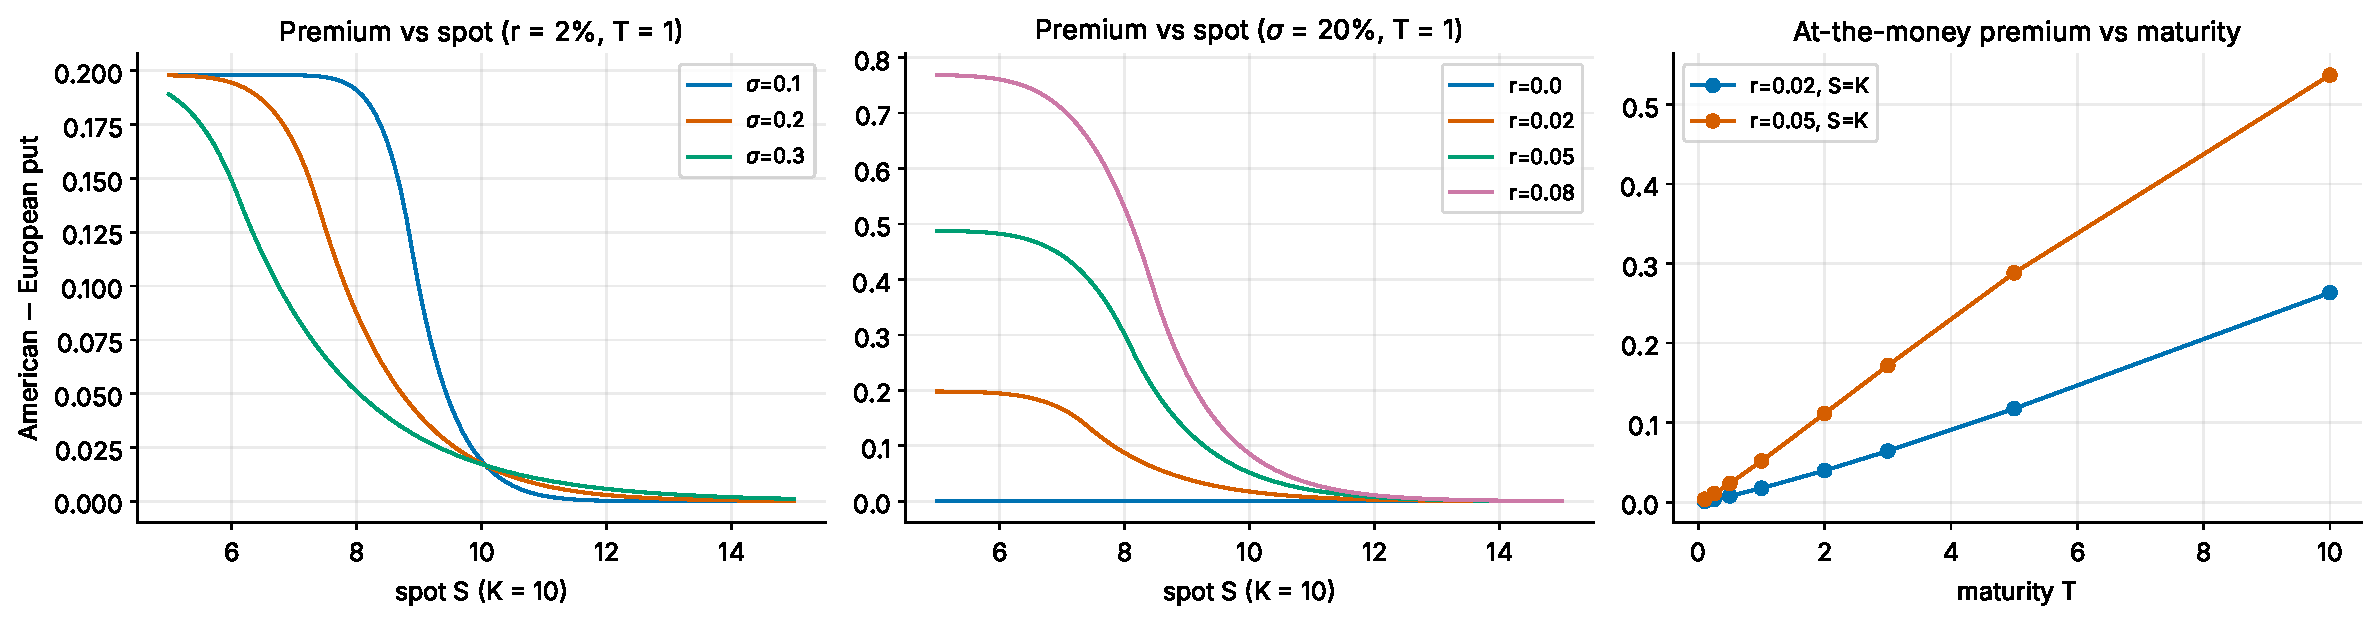
\includegraphics[width=\textwidth]{eep_curves.pdf}
\caption{American minus European put on the same lattice, against spot (left, middle) and maturity (right).\label{fig:eepcurves}}
\end{figure}

\begin{figure}[h!]
\centering
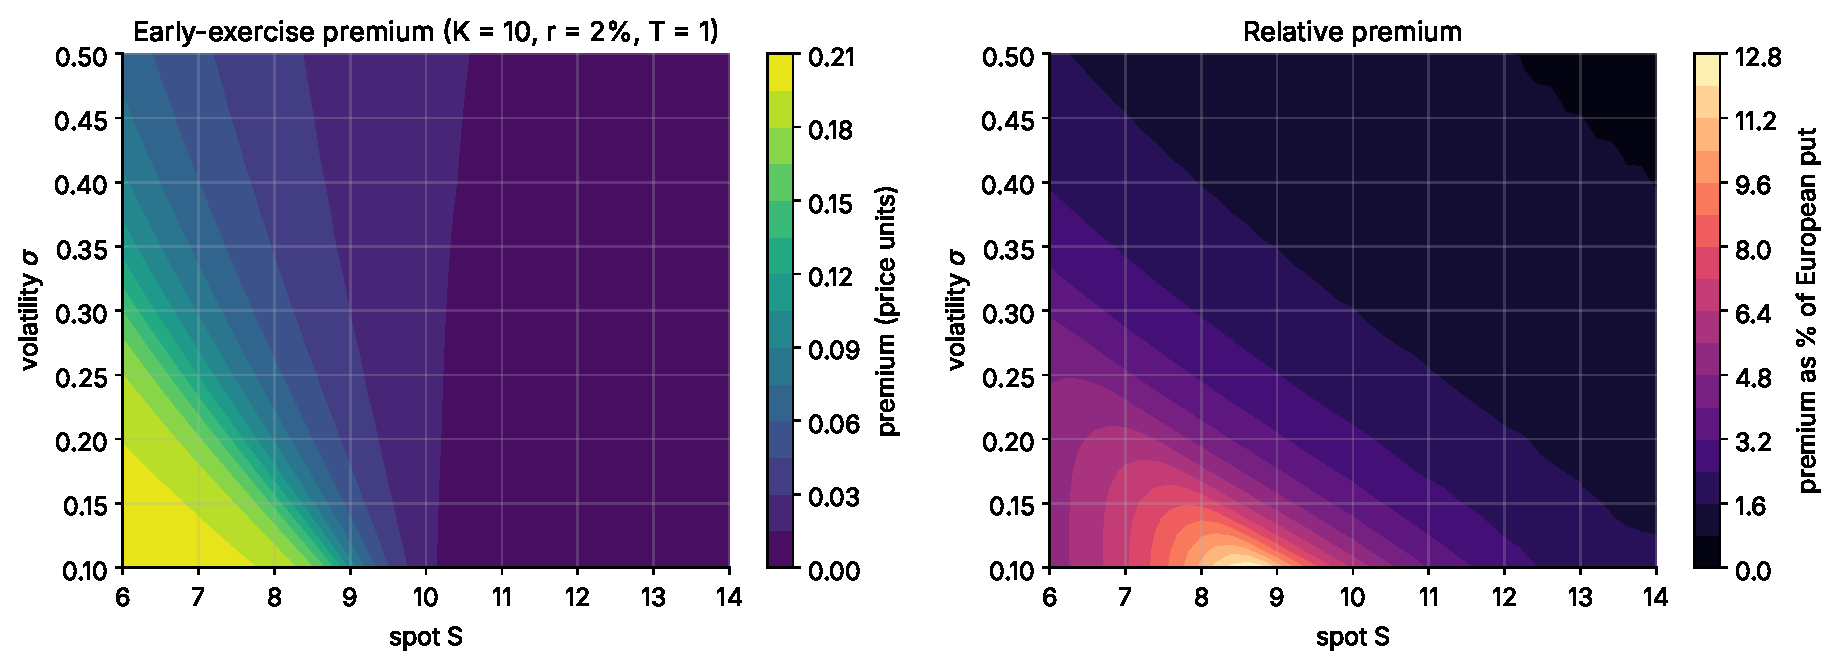
\includegraphics[width=\textwidth]{eep_map.pdf}
\caption{Early-exercise premium in price units (left) and as a percentage of the European put (right).\label{fig:eepmap}}
\end{figure}

\subsection{Dividends}\label{sec:div}
% P44 | 5.7 Early-exercise premium | Result: dividends make early exercise of a call worthwhile
% guide: dev_notes/paragraph_guides/P44_result_dividends_make_early_exercise_of_a_call_w.txt
A continuous dividend yield $q$ lowers the risk-neutral drift of the stock to $r-q$, so the tree uses $p=(e^{(r-q)\Delta t}-d)/(u-d)$ while discounting stays at $r$.
The subclass \texttt{CRRTreeGen} changes only this probability and the payoff, so the boundary, the hedge and the stopping rule are inherited from \texttt{CRRTree}.
With $q=0$ the tree never exercises the American call early, and its price equals the European price on the same lattice.
This is the classical result that early exercise of a call is never optimal without dividends.
Table~\ref{tbl:div} shows that the premium grows with the yield, from zero to \DivPremSix\ at $q=6\%$.
The exercise region of a call is $\{x\ge b(t)\}$ with $b(t)$ above the strike, and Figure~\ref{fig:divboundary} shows that the boundary comes down as the yield rises.
The intuition is that waiting costs the dividends $qS$ per year and earns interest $rK$ on the deferred strike payment, so early exercise becomes attractive when the yield is large relative to the interest rate.


\begin{table}[h!]
\centering
\begin{tabular}{ccccc}
\toprule
dividend yield $q$ & European call (BS) & American call (tree) & premium & $b(0.5)$ \\
\midrule
0\% & 14.2313 & 14.2276 & +0.0000 & -- \\
2\% & 13.0203 & 13.0167 & +0.0000 & 288.8 \\
4\% & 11.8833 & 11.9258 & +0.0461 & 162.9 \\
6\% & 10.8186 & 11.0438 & +0.2287 & 146.5 \\
\bottomrule
\end{tabular}

\caption{European and American call with continuous dividend yield $q$ ($S_0=K=100$, $\sigma=30\%$, $r=5\%$, $T=1$, $M=800$). The premium is American minus European on the same lattice.\label{tbl:div}}
\end{table}

\begin{figure}[h!]
\centering
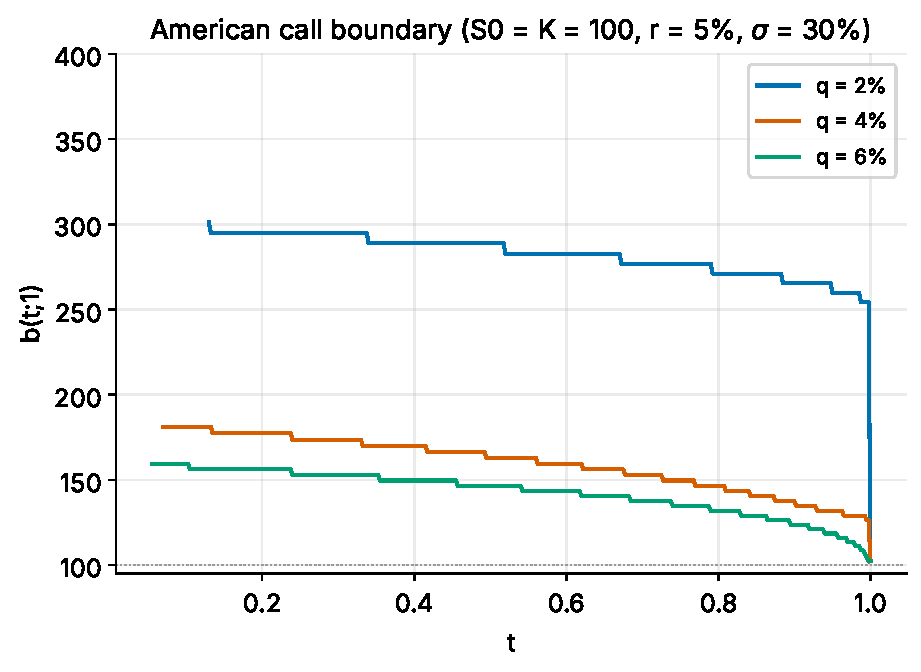
\includegraphics[width=0.55\textwidth]{dividend_boundary.pdf}
\caption{Exercise boundary of the American call for three dividend yields.\label{fig:divboundary}}
\end{figure}

\subsection{An American put on the NVIDIA inputs}\label{sec:nvdaput}
% P45 | 5.7 Early-exercise premium | Result: an American put on the NVIDIA inputs
% guide: dev_notes/paragraph_guides/P45_result_an_american_put_on_the_nvidia_inputs.txt
Put--call parity applied to the Black--Scholes call of Part B gives a European put of \$\NvdaPutEu, which agrees with the direct formula to \ParityNvda.
The American put is worth \$\NvdaPutAm, an early-exercise premium of \$\NvdaPutEEP\ or \NvdaPutEEPpct\% of the European put.
Read as a European put, the American price implies a volatility of \NvdaPutIV\%, which is \NvdaPutIVup\ volatility points above the $37.73\%$ of the model.
A trader who quotes the American put in implied volatility would therefore quote it slightly higher than the European one for the same stock.
The delta of the American put is \NvdaPutDelta\ against \NvdaPutDeltaEu\ for the European put, and the vega is almost the same.
Rho and theta differ more, because the right to exercise early shortens the effective life of the option and reduces its exposure to the interest rate.
At $t=0.5$ the exercise boundary is $\$\NvdaBhalf$, which is \NvdaBhalfPct\% of the strike, far below the $79\%$ of the baseline because the volatility is almost twice as high.
Figure~\ref{fig:boundaryregimes} shows the boundary divided by the strike for five volatility and rate regimes, and Figure~\ref{fig:amgreeks} the value, delta and gamma of the American and European put against the spot.


\begin{table}[h!]
\centering
\begin{tabular}{lcc}
\toprule
 & European put (BS) & American put (tree) \\
\midrule
price & 31.9207 & 32.5674 \\
$\Delta$ & -0.39531 & -0.40708 \\
$\Gamma$ & 0.0042732 & 0.0044968 \\
vega & 92.007 & 92.069 \\
$\Theta$ (per year) & -13.69 & -14.5 \\
$\rho$ & -126.36 & -99.365 \\
\bottomrule
\end{tabular}

\caption{European and American put on the NVIDIA inputs of Part B (Greeks of the American put from the tree, $N=1000$).\label{tbl:nvdaput}}
\end{table}

\begin{figure}[h!]
\centering
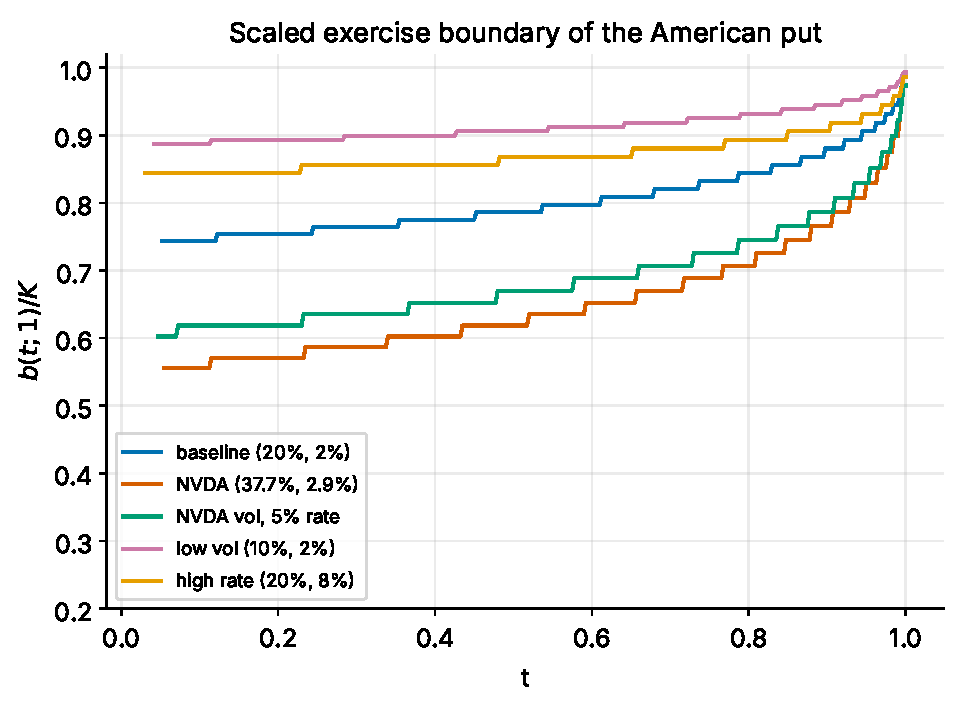
\includegraphics[width=0.6\textwidth]{boundary_regimes.pdf}
\caption{Exercise boundary divided by the strike for five volatility and rate regimes.\label{fig:boundaryregimes}}
\end{figure}

\begin{figure}[h!]
\centering
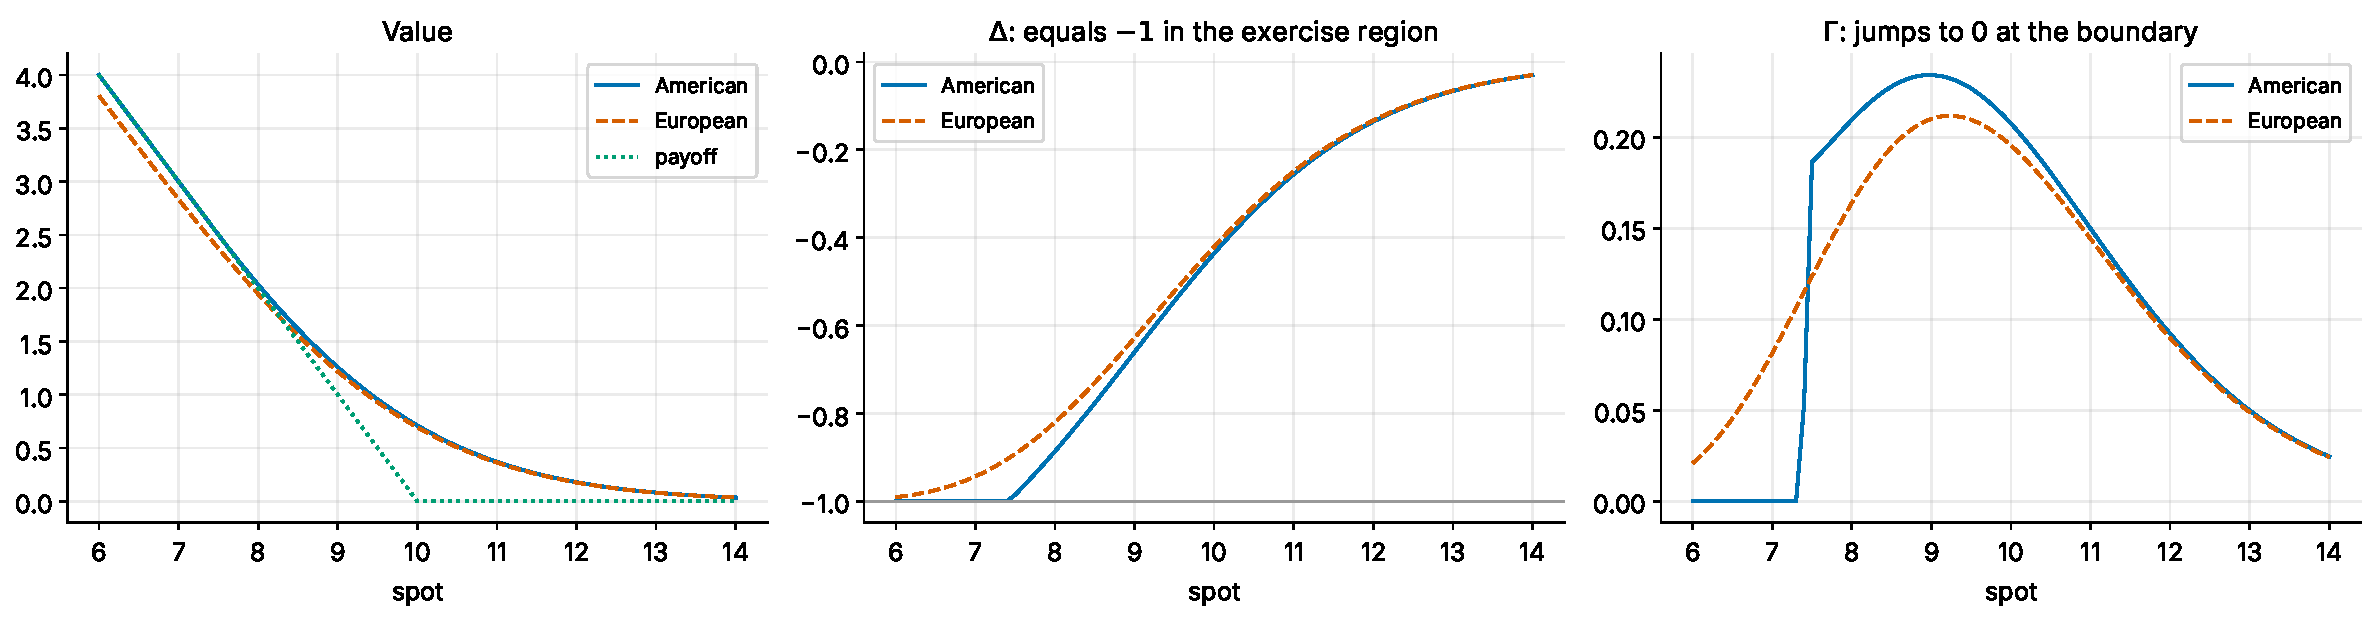
\includegraphics[width=\textwidth]{am_greeks.pdf}
\caption{Value, delta and gamma of the American and European put against spot at $t=0$ (baseline).\label{fig:amgreeks}}
\end{figure}
\FloatBarrier

\subsection{Profit and loss of the buyer}\label{sec:C-pnl}
% P46 | 5.8 Profit and loss | Result: the buyer's profit and loss under the pricing measure
% guide: dev_notes/paragraph_guides/P46_result_the_buyer_s_profit_and_loss_under_the_pri.txt
The buyer pays the fair value $V(0,S_0)=\AmVzero$ and exercises at the first date on which the path enters the exercise region.
Paths are simulated in the tree with the pricing weights $(p,1-p)$, because under the pricing measure the real-world drift $\mu$ plays no role.
The mean profit is \PnLmean\ with a standard error of \PnLse, consistent with zero, as it must be by the definition of the fair value.
A vectorised run with $10^5$ paths gives \PnLQmean\ with a standard error of \PnLQse, which confirms it.
The standard deviation of the profit is \PnLsd, the mean stopping time is \PnLtau\ years and the probability of exercising before maturity is \PnLpex.
Roughly half of the paths are therefore stopped early.
The distribution in Figure~\ref{fig:3a} has a point mass at $-V_0$ for the paths that end out of the money and a long right tail, and Table~\ref{tbl:pnlgrid} repeats the experiment on the nine $(\sigma,r)$ combinations.
The spread grows with $\sigma$ and shrinks with $r$, the probability of early exercise rises with $\sigma$, and for $r=0$ the option is never exercised early, so that $\tau=T$.


\begin{figure}[h!]
\centering
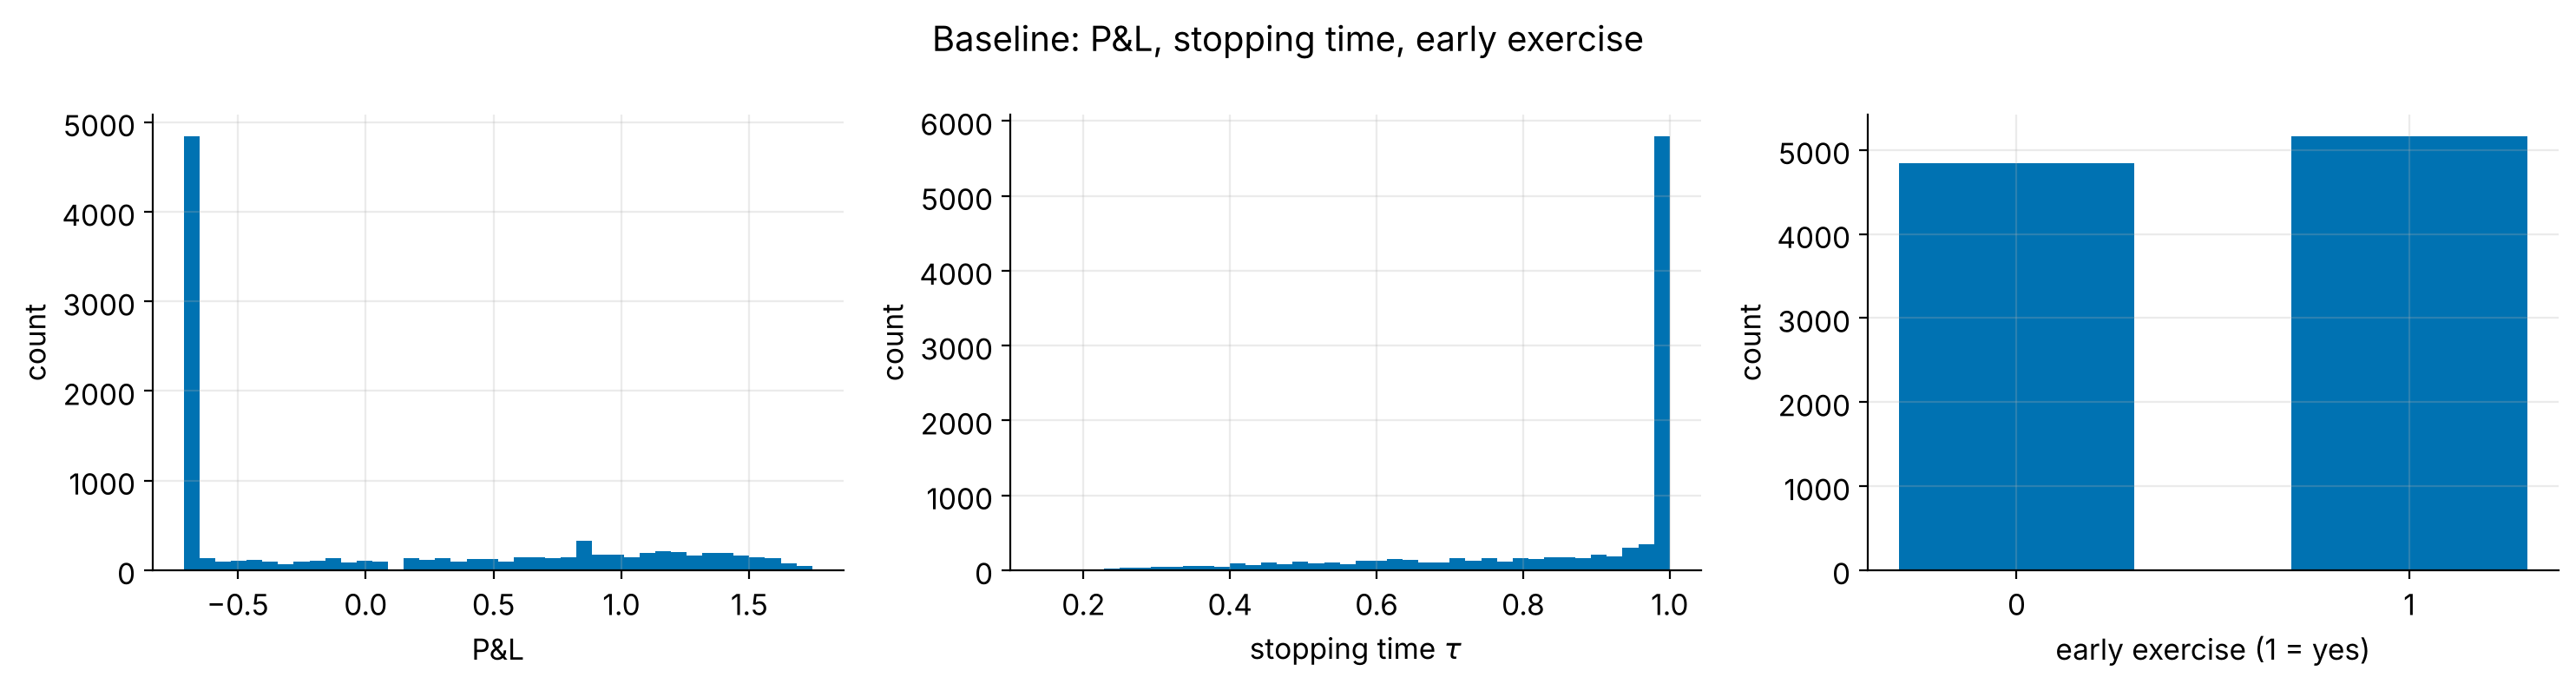
\includegraphics[width=0.9\textwidth]{3a_baseline.png}
\caption{Baseline profit and loss, stopping time and early-exercise indicator, $10{,}000$ paths.\label{fig:3a}}
\end{figure}

\begin{table}[h!]
\centering
\begin{tabular}{ccccc}
\toprule
$\sigma$ & $r$ & mean P\&L (sd) & mean $\tau$ & $p_{ex}$ \\
\midrule
0.1 & 0 & -0.005 (0.546) & 1.000 & 0.000 \\
0.1 & 0.02 & -0.002 (0.391) & 0.854 & 0.473 \\
0.1 & 0.04 & -0.003 (0.324) & 0.808 & 0.444 \\
0.2 & 0 & -0.009 (1.031) & 1.000 & 0.000 \\
0.2 & 0.02 & -0.004 (0.831) & 0.877 & 0.516 \\
0.2 & 0.04 & -0.004 (0.742) & 0.843 & 0.496 \\
0.3 & 0 & -0.012 (1.461) & 1.000 & 0.000 \\
0.3 & 0.02 & -0.001 (1.236) & 0.883 & 0.543 \\
0.3 & 0.04 & -0.007 (1.135) & 0.855 & 0.529 \\
\bottomrule
\end{tabular}

\caption{Profit and loss and exercise statistics, $10{,}000$ paths each.\label{tbl:pnlgrid}}
\end{table}

\begin{figure}[h!]
\begin{minipage}{0.48\textwidth}\centering
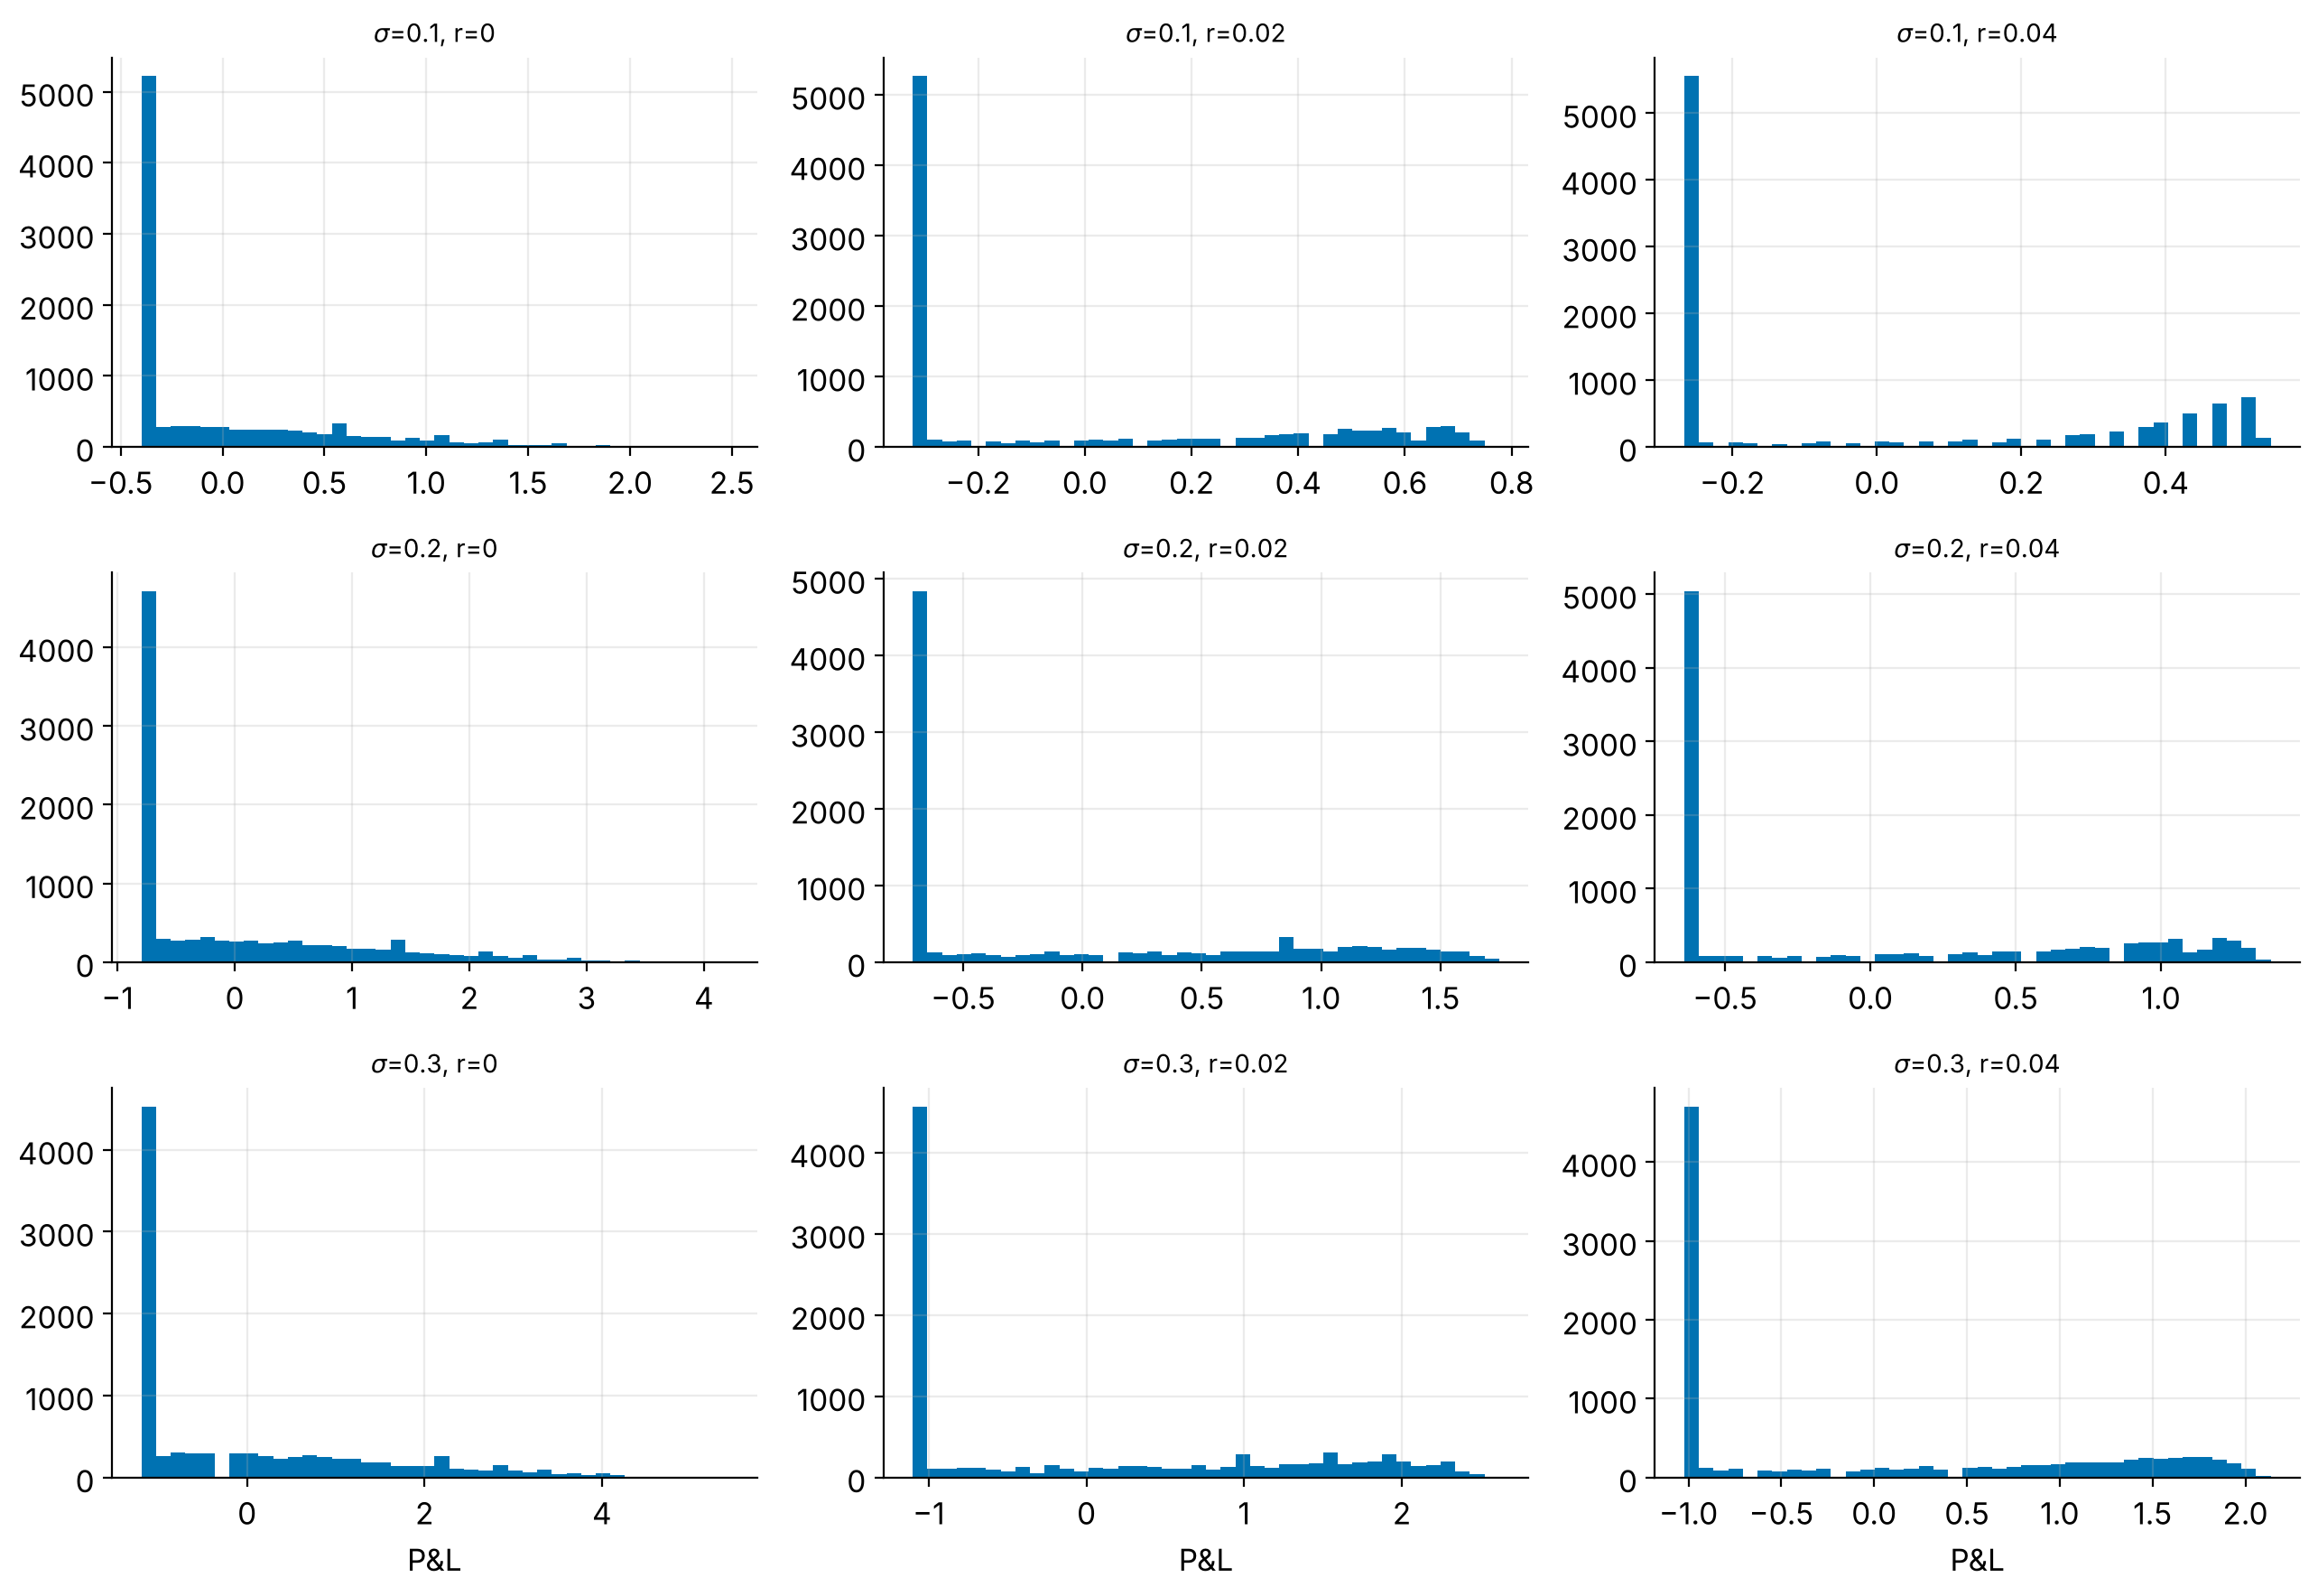
\includegraphics[width=\textwidth]{3b_pnl_grid.png}
\caption{P\&L histograms (rows $\sigma$, columns $r$).\label{fig:3b}}
\end{minipage}\hfill
\begin{minipage}{0.48\textwidth}\centering
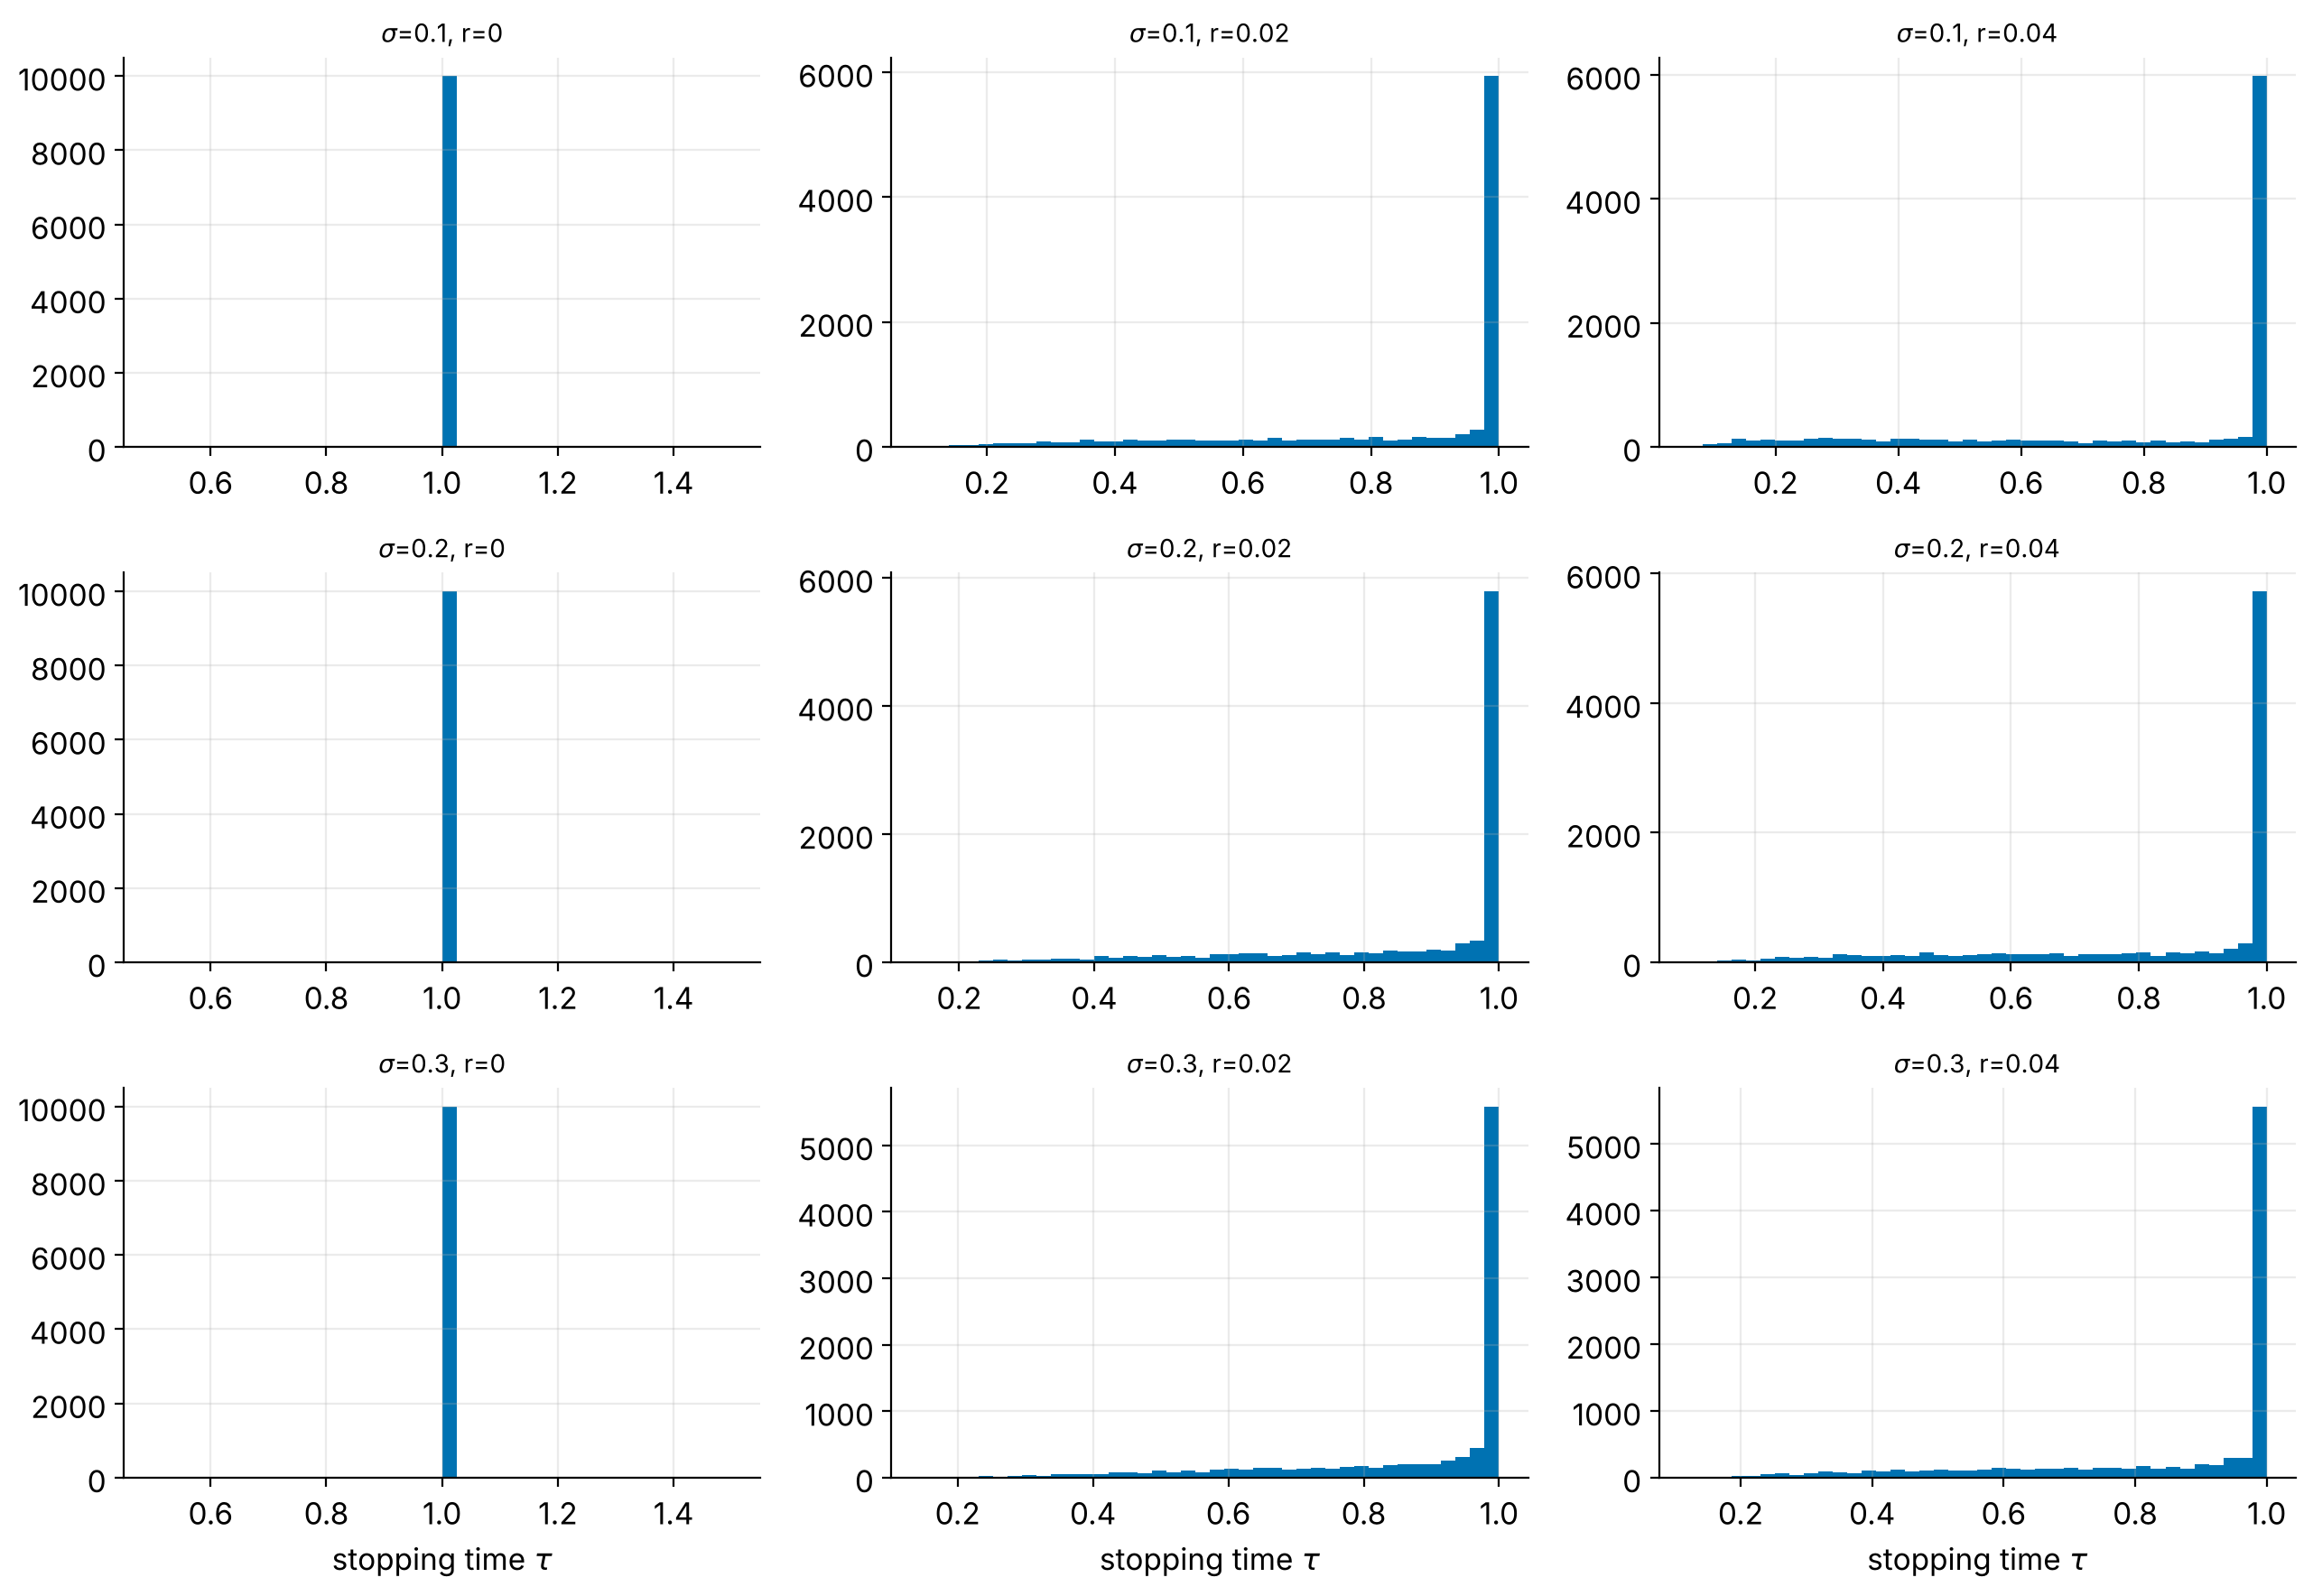
\includegraphics[width=\textwidth]{3b_tau_grid.png}
\caption{Stopping times (rows $\sigma$, columns $r$).\label{fig:3bt}}
\end{minipage}
\end{figure}

% P47 | 5.8 Profit and loss | Result: profit and loss under the real-world measure, and tail risk
% guide: dev_notes/paragraph_guides/P47_result_profit_and_loss_under_the_real_world_meas.txt
Under a real-world drift of $\mu=5\%$ the mean profit of the buyer is \PnLPmean, and at $\mu=10\%$ it is \PnLPmeanTen.
A drift above the risk-free rate makes the stock rise faster than under the pricing measure, so the put pays out less often than the price assumes.
The probability that the buyer loses the entire premium rises from \PnLQtot\% under the pricing measure to \PnLPtot\% at $\mu=5\%$.
The probability of exercising early falls to \PnLPpex, and the mean stopping time rises to \PnLPtau\ years.
The buyer's loss is capped at the premium, so the tail risk is on the seller's side, where the loss equals the buyer's profit.
The $99\%$ quantile of the buyer's profit is \PnLPqNinetyNine\ under the real-world measure and \PnLQqNinetyNine\ under the pricing measure, and the expected shortfall at $95\%$ is \PnLPes\ against \PnLQes, so the right tail hardly moves.
The real-world drift changes how often the put pays out, not how much it pays, which is why the mean moves while the tail does not.
A seller who hedges dynamically is insulated from the drift, as Section~\ref{sec:hedge} showed for the call, whereas an unhedged seller keeps the drift risk.


\begin{table}[h!]
\centering
\resizebox{\textwidth}{!}{\begin{tabular}{lcccccccc}
\toprule
Measure & mean & sd & P(lose premium) & 95\% quantile & 99\% quantile & ES$_{95\%}$ & mean $\tau$ & $p_{ex}$ \\
\midrule
risk-neutral, $\mu=r=2\%$ & -0.003 & 0.834 & 48.8\% & 1.463 & 1.632 & 1.561 & 0.876 & 0.512 \\
real world, $\mu=5\%$ & -0.094 & 0.807 & 54.4\% & 1.407 & 1.632 & 1.542 & 0.894 & 0.456 \\
real world, $\mu=10\%$ & -0.246 & 0.739 & 64.1\% & 1.349 & 1.577 & 1.498 & 0.922 & 0.359 \\
real world, $\mu=-5\%$ & +0.241 & 0.869 & 35.3\% & 1.520 & 1.633 & 1.601 & 0.825 & 0.647 \\
\bottomrule
\end{tabular}
}
\caption{Buyer's profit and loss under the pricing measure and under four real-world drifts ($10^5$ paths each); the buyer pays the $\mathbb Q$-price and exercises on the $\mathbb Q$-boundary. The tail columns are those of the buyer's profit, which is the seller's loss.\label{tbl:pnlreal}}
\end{table}

\begin{figure}[h!]
\centering
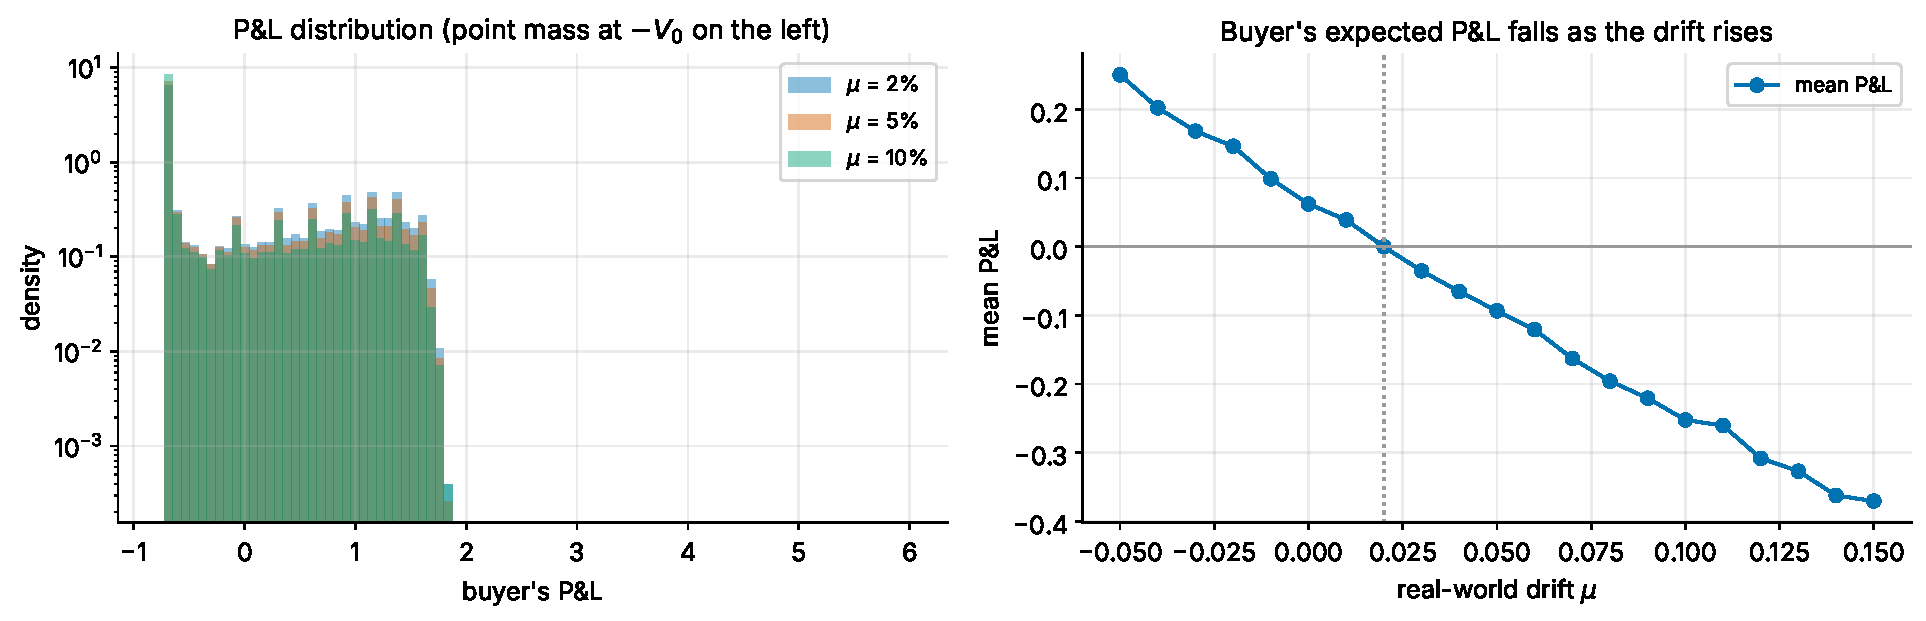
\includegraphics[width=\textwidth]{pnl_real_world.pdf}
\caption{Left: distribution of the buyer's profit under three drifts (log density). Right: mean profit against the real-world drift.\label{fig:pnlreal}}
\end{figure}

\subsection{Mis-specified volatility}\label{sec:misspec}
% P48 | 5.9 Mis-specified volatility | Result: pricing at 20 percent when the realised volatility differs
% guide: dev_notes/paragraph_guides/P48_result_pricing_at_20_percent_when_the_realised_v.txt
Because the boundary $b(t;T)$ decreases in $\sigma$, the $20\%$ boundary lies below the optimal one when the realised volatility is lower than $20\%$, so the buyer exercises too late.
When the realised volatility is higher the $20\%$ boundary lies above the optimal one, and the buyer exercises too early.
At a realised volatility of $10\%$ the mean stopping time is \MisLowTau\ against \MisLowTauOpt\ for the optimal rule, and the buyer loses \MisLowLoss\ relative to optimal exercise.
Waiting too long costs a modest amount because the option is still close to the money.
At $30\%$ the mean stopping time is \MisHighTau\ against \MisHighTauOpt, and the loss relative to optimal exercise is \MisHighLoss.
Exercising too early therefore costs more than exercising too late by a factor of more than two in this example.
The mean profit itself, \MisLowPnL\ at $10\%$ and \MisHighPnL\ at $30\%$, is driven mostly by the price mismatch, since the option is worth less or more than the buyer paid.
The differences relative to the optimal rule are estimated with a standard error of up to \RegretSE\ at $10{,}000$ paths, so the loss at $10\%$ is only about two standard errors, which the next section tightens with ten times more paths.


\begin{table}[h!]
\centering
\resizebox{\textwidth}{!}{\begin{tabular}{ccccccc}
\toprule
$\sigma_{real}$ & mean P\&L & sd & mean $\tau$ & $p_{ex}$ & $\Delta$P\&L vs optimal (s.e.) & $\Delta\tau$ vs optimal \\
\midrule
0.10 & -0.407 & 0.471 & 0.977 & 0.411 & -0.016 (0.003) & +0.123 \\
0.15 & -0.201 & 0.686 & 0.936 & 0.454 & -0.004 (0.003) & +0.067 \\
0.20 & -0.004 & 0.831 & 0.877 & 0.516 & +0.000 (0.000) & +0.000 \\
0.25 & +0.184 & 0.942 & 0.825 & 0.549 & -0.006 (0.004) & -0.056 \\
0.30 & +0.353 & 1.002 & 0.766 & 0.590 & -0.036 (0.007) & -0.118 \\
\bottomrule
\end{tabular}
}
\caption{Following the $\sigma=20\%$ boundary when the realised volatility differs; $\Delta$ is relative to the optimal rule of the realised volatility on the same paths.\label{tbl:misspec}}
\end{table}

\begin{figure}[h!]
\centering
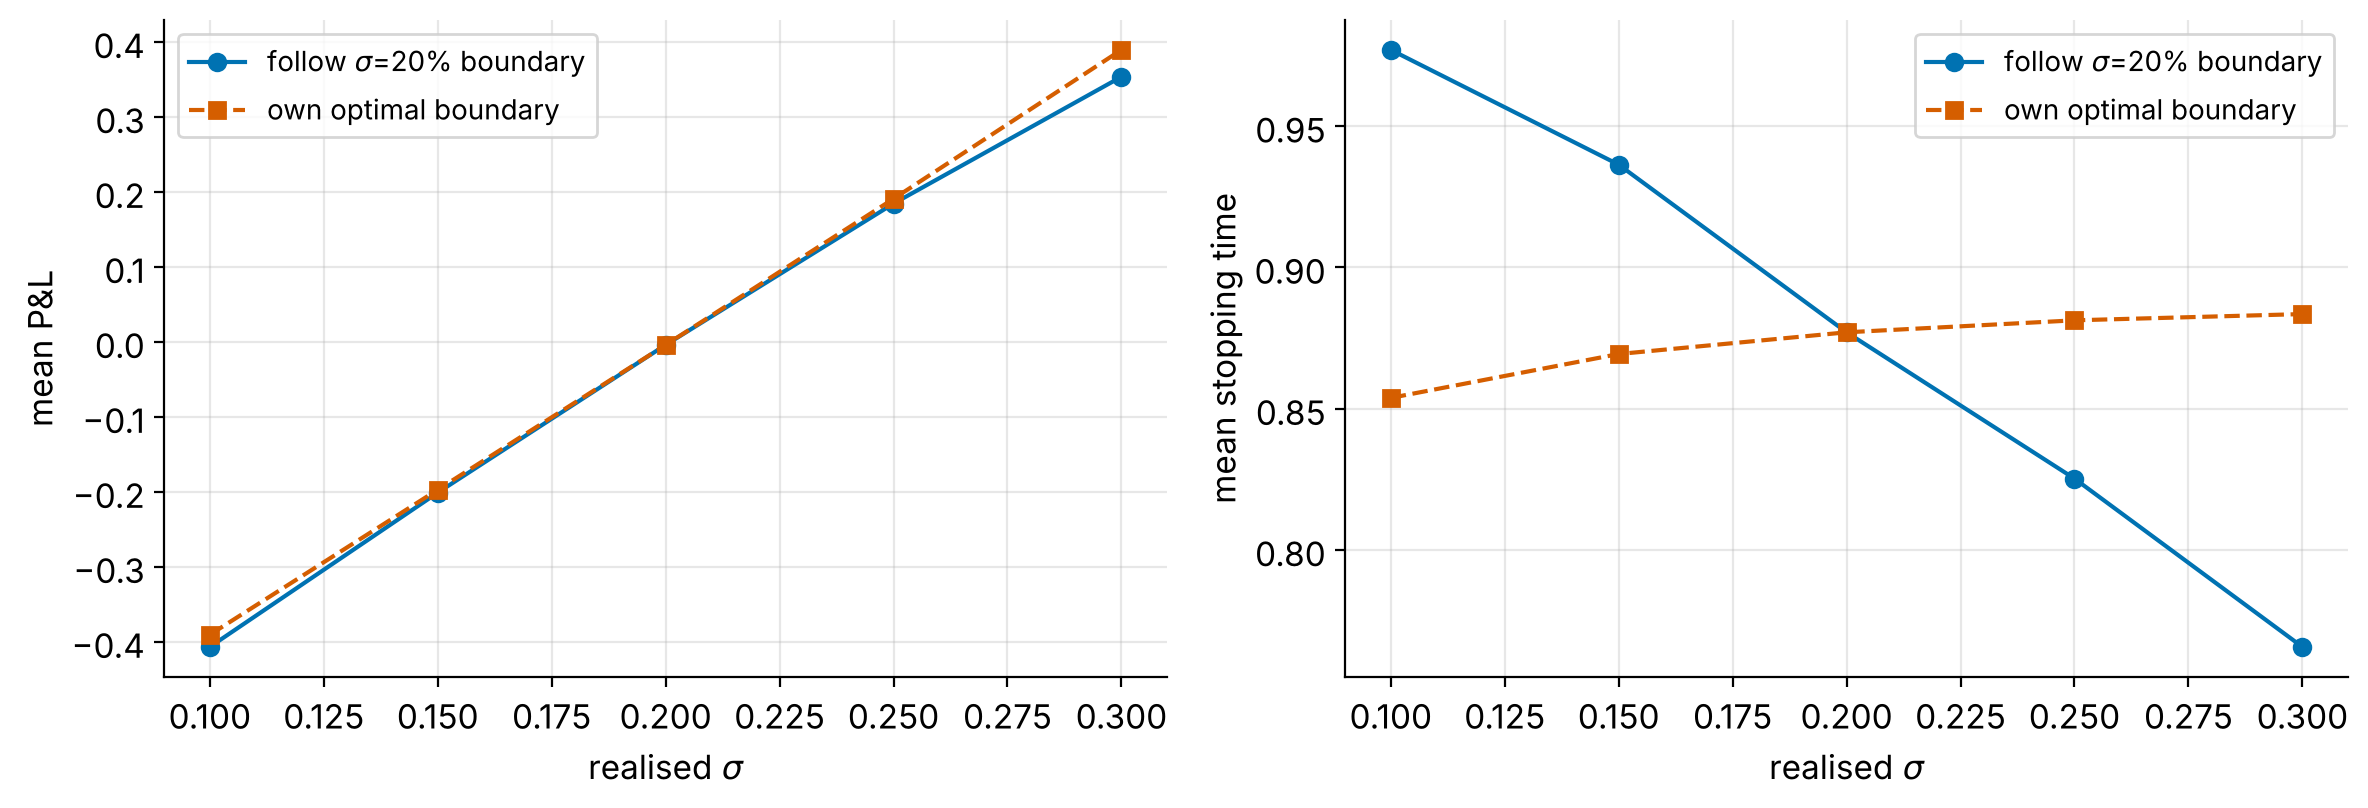
\includegraphics[width=0.75\textwidth]{3c_summary.png}
\caption{Mean profit and mean stopping time against the realised volatility.\label{fig:3c}}
\end{figure}

% P49 | 5.9 Mis-specified volatility | Result: the full map of priced against realised volatility
% guide: dev_notes/paragraph_guides/P49_result_the_full_map_of_priced_against_realised_v.txt
The buyer's mean profit splits into the premium mismatch, the difference between the value under the realised volatility and the price paid, and the policy regret, the loss from using the wrong boundary.
The first term is first-order in the volatility gap, roughly the vega of the put (about \AmVegaTree\ per unit of volatility) times the gap, and the second is second-order.
The regret matrix in Figure~\ref{fig:misspecmap} is strongly asymmetric: the largest regret, \MapRegretLowHigh, occurs when the price is set at $10\%$ and the realised volatility is $30\%$, so that the buyer exercises too early.
In the opposite corner, priced at $30\%$ and realised at $10\%$, the buyer exercises too late and the regret is only \MapRegretHighLow.
The asymmetry has a simple reason: exercising too early gives up an option whose value is large when volatility is high, whereas waiting too long costs only the interest on the strike and some time value.
The ratio between the two corners is about twenty.
Each cell uses \MapPaths\ paths, so the standard error of the regret is at most \MapSE, which is small compared with the large entries and comparable with the small ones.
In the corner priced at $10\%$ and realised at $30\%$ the buyer's mean profit is \MapPnLmismatch, mostly because the option was bought cheaply, which shows that the premium mismatch dominates the regret.


\begin{figure}[h!]
\centering
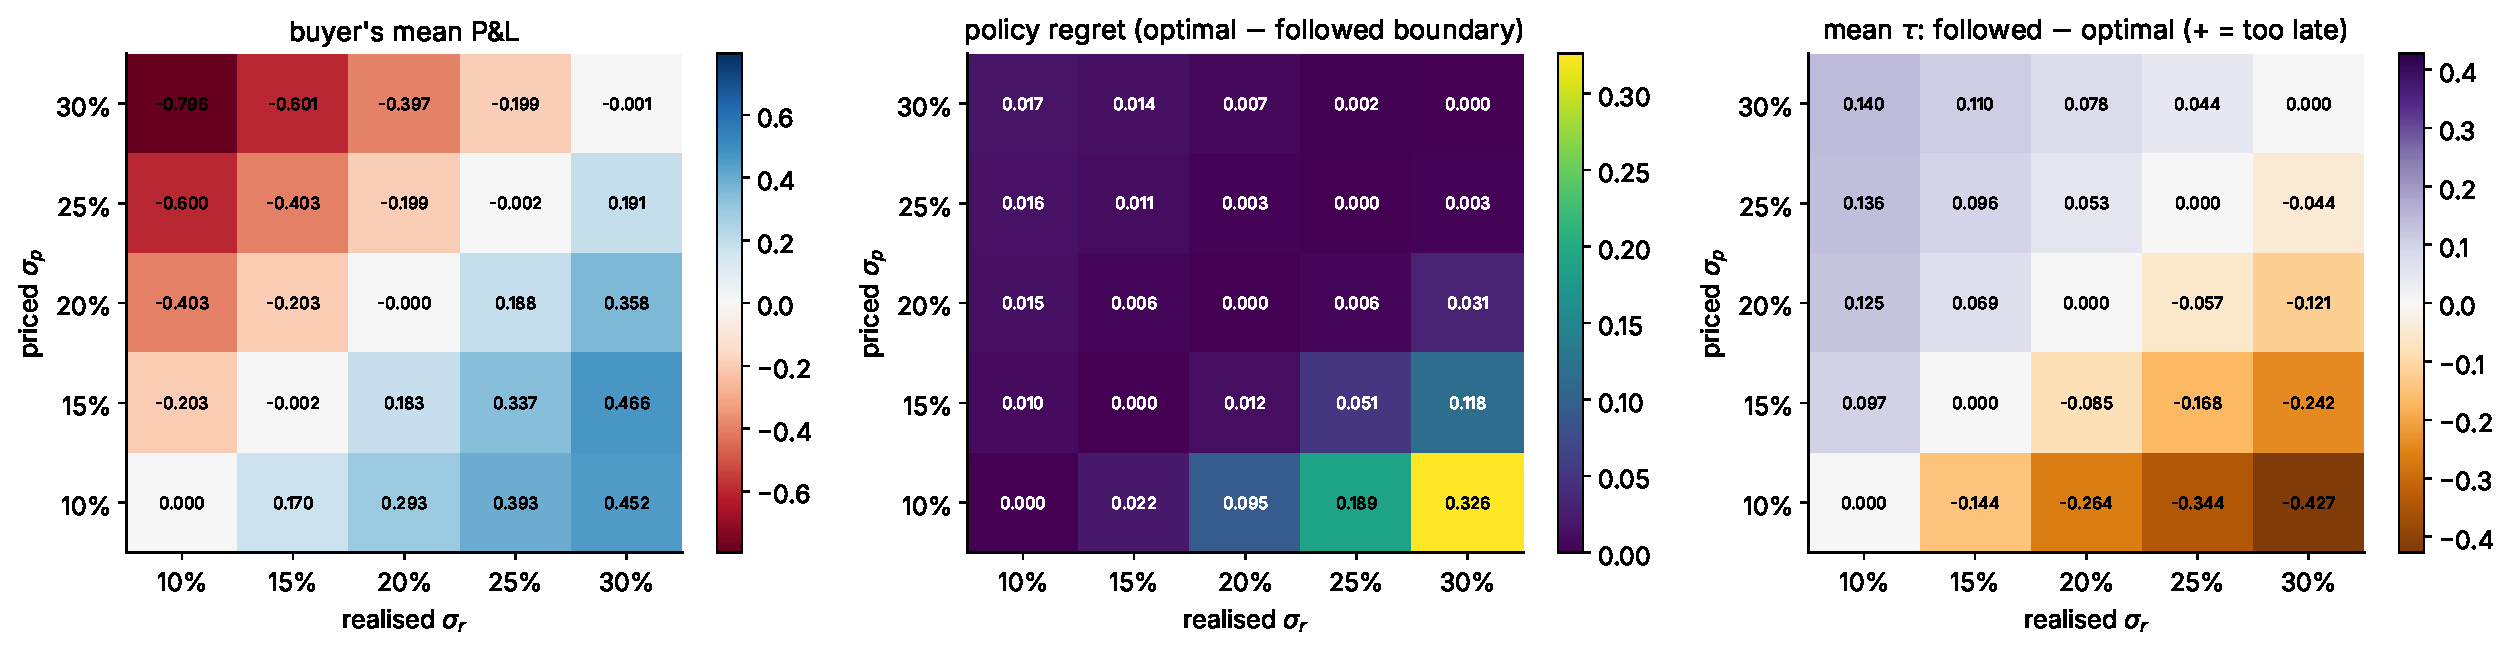
\includegraphics[width=\textwidth]{misspec_map.pdf}
\caption{Rows: priced volatility; columns: realised volatility. Left: buyer's mean profit. Middle: policy regret. Right: mean stopping time of the followed rule minus the optimal one (positive: too late).\label{fig:misspecmap}}
\end{figure}

\begin{table}[h!]
\centering
\resizebox{\textwidth}{!}{\begin{tabular}{lccccc}
\toprule
priced $\sigma_p$ & real. 10\% & real. 15\% & real. 20\% & real. 25\% & real. 30\% \\
\midrule
10\% & +0.000 / 0.000 & +0.170 / 0.022 & +0.293 / 0.095 & +0.393 / 0.189 & +0.452 / 0.326 \\
15\% & -0.203 / 0.010 & -0.002 / 0.000 & +0.183 / 0.012 & +0.337 / 0.051 & +0.466 / 0.118 \\
20\% & -0.403 / 0.015 & -0.203 / 0.006 & -0.000 / 0.000 & +0.188 / 0.006 & +0.358 / 0.031 \\
25\% & -0.600 / 0.016 & -0.403 / 0.011 & -0.199 / 0.003 & -0.002 / 0.000 & +0.191 / 0.003 \\
30\% & -0.796 / 0.017 & -0.601 / 0.014 & -0.397 / 0.007 & -0.199 / 0.002 & -0.001 / 0.000 \\
\bottomrule
\end{tabular}
}
\caption{Mean profit / policy regret for each pair of priced (rows) and realised (columns) volatility, $10^5$ paths per cell.\label{tbl:misspecmap}}
\end{table}

% P50 | 5 Part C summary | What Part C shows about the American put
% guide: dev_notes/paragraph_guides/P50_what_part_c_shows_about_the_american_put.txt
The CRR tree, a finite-difference solver for the variational inequality and least-squares Monte Carlo agree with each other within their numerical errors, and the tree approaches the closed-form perpetual put as the maturity and the number of steps grow.
The one row that disagreed, $T=1000$ with $800$ steps, was a lattice artefact, and the refined computation says so.
Early exercise adds a few percent to an at-the-money put and much more deep in the money, and it is zero for $r=0$ and for calls without dividends.
For the NVIDIA put it adds about \NvdaPutEEPpct\% to the European price.
The buyer's expected profit under the real-world measure depends on the drift, which the price does not.
A wrong volatility corrupts the exercise rule asymmetrically, because exercising too early costs much more than exercising too late.
In practice the tree is the natural tool for prices, boundaries and hedges, a PDE solver is better when accuracy is needed in one or two dimensions, regression Monte Carlo takes over when the dimension is high, and Barone--Adesi--Whaley serves for a quick estimate.

\FloatBarrier

% ======================================================================================== 6
\section{Comparison of methods}\label{sec:compare}
% P51 | 6 Comparison of methods | Result: the European call on one footing
% guide: dev_notes/paragraph_guides/P51_result_the_european_call_on_one_footing.txt
Table~\ref{tbl:deskcall} shows that the vectorised CRR tree with $N=252$ reproduces the price of the list-based class, with an error of \DeskCrrVecErr, in \DeskCrrVecMs\ ms instead of \DeskCrrClassMs\ ms.
The Leisen--Reimer tree with $N=101$ has an error of \$\DeskLrErr\ in \DeskLrMs\ ms, and CRR with smoothing and Richardson extrapolation at $N=252$ has an error of \$\DeskSmoothErr.
Plain Monte Carlo with $10^5$ samples has a standard error of \$\DeskMcPlainSE\ (the realised error is \$\DeskMcPlainErr) and takes \DeskMcPlainMs\ ms.
The control variate brings the standard error to \$\DeskMcCvSE\ at the same cost, and scrambled Sobol points with $2^{16}$ samples reach an error of \$\DeskSobolErr\ in \DeskSobolMs\ ms.
The Euler--Maruyama simulation with $252$ steps takes about \DeskMcEulerMs\ ms for the same $10^5$ samples, roughly two orders of magnitude more than the exact sampler, and has the same standard error.
For a European payoff on geometric Brownian motion the extra cost buys nothing, because the exact terminal law is known; the scheme earns its place when the dynamics are not solvable.
The order of the rows is stable across machines, but the absolute times are not and should be read as orders of magnitude.


\begin{table}[h!]
\centering
\resizebox{\textwidth}{!}{\begin{tabular}{lcccr}
\toprule
Method & price & error vs BS & s.e. & CPU (ms) \\
\midrule
Black-Scholes closed form & 38.7493 & +0.0000 & -- & 0.2 \\
CRR tree, $N=252$ (class, lists) & 38.7142 & -0.0350 & -- & 11.8 \\
CRR tree, $N=252$ (vectorised) & 38.7142 & -0.0350 & -- & 0.6 \\
CRR tree, $N=1000$ (vectorised) & 38.7404 & -0.0088 & -- & 3.4 \\
CRR + smoothing + Richardson, $N=252$ & 38.7493 & +0.0000 & -- & 2.5 \\
Leisen-Reimer tree, $N=101$ & 38.7491 & -0.0002 & -- & 0.2 \\
Monte Carlo plain, $M=10^5$ (exact sampler) & 38.5401 & -0.2092 & 0.2155 & 3.5 \\
Monte Carlo control variate, $M=10^5$ & 38.6810 & -0.0682 & 0.0821 & 3.4 \\
Monte Carlo Euler $N=252$, $M=10^5$ & 38.6841 & -0.0652 & 0.2156 & 398.1 \\
Scrambled Sobol QMC, $2^{16}$ points & 38.7479 & -0.0013 & -- & 2.6 \\
\bottomrule
\end{tabular}
}
\caption{European call: every method on one footing (single core; the CPU time is the fastest of several runs for the quick methods).\label{tbl:deskcall}}
\end{table}

% P52 | 6 Comparison of methods | Result: work-precision for the European call
% guide: dev_notes/paragraph_guides/P52_result_work_precision_for_the_european_call.txt
Figure~\ref{fig:workprecision} plots the error of each method against the CPU time it uses, on logarithmic axes.
The tree errors fall with slope about $-1$ (CRR) or $-2$ (Leisen--Reimer) in the number of steps, the Monte Carlo standard errors fall with slope $-\tfrac12$ in the time, and the Sobol points have a much steeper slope because the integral is one-dimensional.
To bring the error below \$\WPtol, plain CRR needs $N=\WPcrrN$ steps and \WPcrrMs\ ms, CRR with smoothing and Richardson needs $N=\WPsmN$ and \WPsmMs\ ms, and the Leisen--Reimer tree needs $N=\WPlrN$ and \WPlrMs\ ms.
The gap between the first and the last is therefore a factor of several hundred in time.
Plain Monte Carlo needs about $\WPmcM$ samples for a standard error of \$\WPtol, which is about \WPmcSec\ seconds by extrapolation, and the control variate needs about \WPcvSec\ seconds.
Scrambled Sobol points reach the same accuracy with \WPsobolM\ points in a few milliseconds.
This ranking is specific to a one-dimensional European payoff, and it reverses for many underlyings or for path-dependent payoffs, where lattices become infeasible and Monte Carlo keeps its rate.


\begin{figure}[h!]
\centering
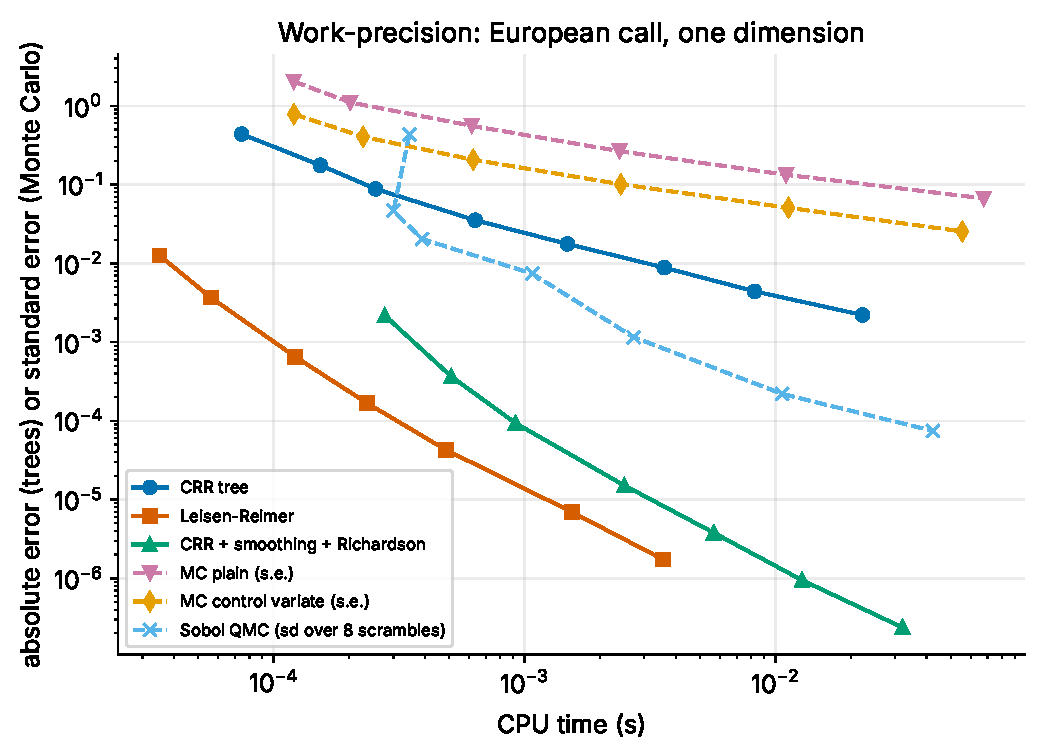
\includegraphics[width=0.75\textwidth]{work_precision.pdf}
\caption{Work--precision diagram for the European call: absolute error of the trees and standard error of the Monte Carlo estimators against CPU time.\label{fig:workprecision}}
\end{figure}

% P53 | 6 Comparison of methods | Result: the American put on one footing
% guide: dev_notes/paragraph_guides/P53_result_the_american_put_on_one_footing.txt
Table~\ref{tbl:deskput} shows that the tree with $M=1600$ steps is within \DeskPutTreeErr\ of the extrapolated reference and takes \DeskPutTreeMs\ ms.
The list-based class needs \DeskPutClassMs\ ms for $800$ steps against \DeskPutVecMs\ ms for the vectorised pricer, and the reference itself costs \DeskPutRefMs\ ms.
The finite-difference solver on a $801\times200$ grid has an error of \DeskPdeCoarseErr\ in \DeskPdeCoarseMs\ ms, and on a $3201\times800$ grid an error of \DeskPdeFineErr\ in \DeskPdeFineMs\ ms.
In one dimension the PDE solver is therefore at least as accurate as the tree for comparable time, and it gives the boundary and the Greeks from the same grid.
Least-squares Monte Carlo has an error of \DeskLsmErr\ against a standard error of \DeskLsmSE\ and takes \DeskLsmMs\ ms, so it is the slowest method here, and its error is of the size of its own statistical noise.
The Barone--Adesi--Whaley approximation is off by \DeskBawErr\ but takes \DeskBawMs\ ms, which is why it remains useful for screening.
Least-squares Monte Carlo is worth having nonetheless, because its cost does not grow exponentially with the number of underlyings, which is the case where the tree and the grid fail.


\begin{table}[h!]
\centering
\resizebox{\textwidth}{!}{\begin{tabular}{lccrr}
\toprule
Method & price & error vs reference & s.e. & CPU (ms) \\
\midrule
European put (Black-Scholes), for reference & 0.69359 & -0.01749 & -- & 0 \\
CRR tree, $M=800$ (class, lists) & 0.71094 & -0.00014 & -- & 24 \\
CRR tree, $M=800$ (vectorised) & 0.71094 & -0.00014 & -- & 15 \\
CRR tree, $M=1600$ (vectorised) & 0.71101 & -0.00007 & -- & 51 \\
CRR tree + Richardson ($M=3200,6400$): reference & 0.71108 & +0.00000 & -- & 533 \\
PDE, Crank-Nicolson + penalty, $801\times200$ & 0.71100 & -0.00008 & -- & 132 \\
PDE, Crank-Nicolson + penalty, $3201\times800$ & 0.71107 & -0.00001 & -- & 1361 \\
Longstaff-Schwartz, 50 dates, $2\cdot10^5$ paths & 0.71267 & +0.00159 & 0.0019 & 1402 \\
Barone-Adesi-Whaley approximation & 0.70999 & -0.00109 & -- & 1 \\
\bottomrule
\end{tabular}
}
\caption{American put (baseline): every method against the Richardson-extrapolated tree.\label{tbl:deskput}}
\end{table}

% P54 | 6 Comparison of methods | Which method for which job
% guide: dev_notes/paragraph_guides/P54_which_method_for_which_job.txt
For a vanilla European option the closed form is the answer when it exists, and otherwise a Leisen--Reimer tree or a smoothed and extrapolated CRR tree is faster and more accurate than any simulation.
Monte Carlo serves there only as an independent cross-check.
For an American option on one underlying a CRR tree with Richardson extrapolation delivers the price, the exercise boundary and the hedge in tens of milliseconds, and a PDE solver is the better choice when high accuracy is needed.
The Barone--Adesi--Whaley formula is good enough for screening and for initialising a root-finder.
For path-dependent payoffs or several underlyings, Monte Carlo with variance reduction is the default, with a regression step such as Longstaff--Schwartz if early exercise is allowed.
The cost of a tree or a grid grows exponentially with the dimension and rules them out beyond two or three underlyings.
Sensitivities come from the same lattice or grid as the price where possible, and from pathwise or likelihood-ratio estimators in Monte Carlo.
A stress of the volatility input is more informative than any refinement of the numerics, because in both parts of this report the effect of a wrong volatility dwarfs the numerical error of a reasonable method.

\FloatBarrier

% ======================================================================================== 7
\section{Conclusions}\label{sec:concl}
% P55 | 7 Conclusions | Conclusions: the European call and the two languages
% guide: dev_notes/paragraph_guides/P55_conclusions_the_european_call_and_the_two_langua.txt
The discrete and the continuous language agree in the limit: the scaled random walk converges to Brownian motion at rate $N^{-1/2}$ in the Kolmogorov distance, and the CRR price converges to the Black--Scholes price at rate $1/N$ with a sign that depends on the parity of $N$.
The sign pattern is a property of the kink at the strike and can be removed.
For a vanilla payoff a well-chosen lattice beats Monte Carlo by orders of magnitude in accuracy per unit of time, and variance reduction recovers only a part of the gap.
The strength of Monte Carlo is its generality, not its accuracy.
The Greeks can be obtained from the closed form, from the tree and from Monte Carlo, and the three agree.
The error of a discrete delta hedge falls only like $n^{-1/2}$ in the number of rebalances, and a wrong hedging volatility costs far more than a coarser schedule.
The point to remember is that, for a reasonable method, the volatility that goes into the model matters more than the numerical scheme that processes it.


% P56 | 7 Conclusions | Conclusions: the American put
% guide: dev_notes/paragraph_guides/P56_conclusions_the_american_put.txt
The CRR tree is an explicit finite-difference scheme for the variational inequality, and the tree, a finite-difference solver and least-squares Monte Carlo agree on the price of the American put.
The perpetual put is the limit of the long-dated put, and the one case that seemed to contradict this, a thousand-year maturity on a coarse lattice, was an artefact of the lattice.
Early exercise adds a few percent at the money and more deep in the money, and it needs a positive interest rate for a put and a dividend for a call.
The boundary falls when volatility rises and rises when the interest rate rises, which is what the cost and the value of waiting predict.
The price does not depend on the real-world drift but the buyer's expected profit does, and a seller who does not hedge carries that dependence.
A wrong volatility corrupts the exercise rule, and the loss is asymmetric: exercising too early costs much more than exercising too late.
In practice the volatility input and the exercise rule should be monitored together, because an error in the first propagates into the second.


% P57 | 7 Conclusions | Limitations and next steps
% guide: dev_notes/paragraph_guides/P57_limitations_and_next_steps.txt
The model assumes a constant volatility, whereas real markets show an implied-volatility smile and term structure, so a local- or stochastic-volatility model would be the natural next step.
The tree would then no longer recombine so simply, and the PDE would gain a second dimension.
The inputs are simplified: a historical volatility instead of an implied one, a Canadian rate for a US-dollar stock, and no dividends for NVIDIA.
In practice each of these would be replaced by market data, and the sensitivities of Section~\ref{sec:B-greeks} say how much the price would move.
There are no transaction costs and no jumps in the model, and discrete hedging is studied only for the call.
Jump or gap risk would leave a residual that no rebalancing frequency removes.
Natural next steps are to calibrate to an option chain, to add a discrete dividend schedule, and to extend the regression Monte Carlo to a basket of underlyings.


% ======================================================================================== appendices
\clearpage
\appendix
\section{Derivations}\label{app:derivations}

\subsection{It\^o's formula and the solution of GBM}
% P58 | Appendix A: derivations | Ito's formula and the solution of GBM
% guide: dev_notes/paragraph_guides/P58_ito_s_formula_and_the_solution_of_gbm.txt
The rules of It\^o calculus follow from the quadratic variation of Brownian motion: $(dt)^2=0$, $dt\,dW=0$ and $(dW)^2=dt$.
For a twice differentiable $f$ and $dS=\mu S\,dt+\sigma S\,dW$ it gives, using $(dS)^2=\sigma^2S^2\,dt$,
\begin{equation}
 df(S_t)=f'(S_t)\,dS_t+\tfrac12f''(S_t)\,\sigma^2S_t^2\,dt .
\end{equation}
With $f=\ln$ one has $f'=1/S$ and $f''=-1/S^2$, so $d\ln S_t=(\mu-\tfrac12\sigma^2)\,dt+\sigma\,dW_t$.
Integrating from $0$ to $t$ and exponentiating gives $S_t=S_0\exp\big((\mu-\tfrac12\sigma^2)t+\sigma W_t\big)$.
To check this, apply It\^o's formula to $g(t,W)=S_0e^{(\mu-\frac12\sigma^2)t+\sigma W}$: $dg=(\mu-\tfrac12\sigma^2)g\,dt+\sigma g\,dW+\tfrac12\sigma^2g\,dt=\mu g\,dt+\sigma g\,dW$.
Hence $\ln S_t$ is normal with mean $\ln S_0+(\mu-\tfrac12\sigma^2)t$ and variance $\sigma^2t$, and since $\mathbb E[e^{\sigma W_t}]=e^{\sigma^2t/2}$ one gets $\mathbb E[S_t]=S_0e^{\mu t}$ and $\operatorname{Var}[S_t]=S_0^2e^{2\mu t}\big(e^{\sigma^2t}-1\big)$.
The variance is what sets the size of the Monte Carlo standard errors of Section~\ref{sec:B}.


\subsection{The Black--Scholes formula by direct integration}
% P59 | Appendix A: derivations | The Black-Scholes formula by direct integration
% guide: dev_notes/paragraph_guides/P59_the_black_scholes_formula_by_direct_integration.txt
Under $\mathbb Q$ write $S_T=S_0e^{(r-\frac12\sigma^2)T+\sigma\sqrt TZ}$ with $Z\sim N(0,1)$, so that $C=e^{-rT}\mathbb E[(S_T-K)^+]$.
The payoff is positive exactly when $Z>-d_2$, where $d_2=\frac{\ln(S_0/K)+(r-\frac12\sigma^2)T}{\sigma\sqrt T}$.
Splitting the expectation gives $C=e^{-rT}\big(\mathbb E[S_T\mathbf 1_{\{Z>-d_2\}}]-K\,\mathbb P(Z>-d_2)\big)$.
By symmetry $\mathbb P(Z>-d_2)=\Phi(d_2)$, so the second term is $Ke^{-rT}\Phi(d_2)$.
For the first term, completing the square gives $e^{\sigma\sqrt Tz}\varphi(z)=e^{\sigma^2T/2}\varphi(z-\sigma\sqrt T)$, so
\begin{equation}
 \mathbb E[S_T\mathbf 1_{\{Z>-d_2\}}]=S_0e^{rT}\int_{-d_2}^{\infty}\varphi(z-\sigma\sqrt T)\,dz=S_0e^{rT}\,\Phi(d_2+\sigma\sqrt T)=S_0e^{rT}\,\Phi(d_1).
\end{equation}
Combining the two terms gives Equation~\eqref{eq:bs}: $\Phi(d_2)$ is the risk-neutral probability that the call ends in the money, and $\Phi(d_1)$ is the same probability under the measure that takes the stock as numeraire.


\subsection{The Black--Scholes PDE and the hedging argument}
% P60 | Appendix A: derivations | The Black-Scholes PDE and the hedging argument
% guide: dev_notes/paragraph_guides/P60_the_black_scholes_pde_and_the_hedging_argument.txt
Let $V(t,S_t)$ be the value of the option and consider a portfolio that is short one option and long $\Delta$ shares, so that $\Pi=\Delta S-V$.
We choose $\Delta$ so that the portfolio has no exposure to the Brownian motion.
It\^o's formula gives $dV=V_t\,dt+V_S\,dS+\tfrac12\sigma^2S^2V_{SS}\,dt$ under the real-world dynamics~\eqref{eq:gbm}.
With $\Delta=V_S$ the terms in $dS$ cancel in $d\Pi=\Delta\,dS-dV$, which leaves the deterministic increment $d\Pi=-\big(V_t+\tfrac12\sigma^2S^2V_{SS}\big)\,dt$.
A portfolio without risk must earn the riskless rate, so $d\Pi=r\Pi\,dt=r(SV_S-V)\,dt$.
Equating the two expressions gives the Black--Scholes PDE
\begin{equation}\label{eq:bspde}
 V_t+rSV_S+\tfrac12\sigma^2S^2V_{SS}-rV=0 .
\end{equation}
The real-world drift $\mu$ has disappeared from the equation, which is the continuous-time form of the statement that the price does not depend on $\mu$.
With the terminal condition $V(T,S)=(S-K)^+$ the solution is, by the Feynman--Kac formula, the discounted risk-neutral expectation $e^{-r(T-t)}\mathbb E^{\mathbb Q}[(S_T-K)^+\mid S_t=S]$ of Section~\ref{sec:setting}.


\subsection{Convergence of the CRR tree to geometric Brownian motion}
% P61 | Appendix A: derivations | Convergence of the CRR tree to geometric Brownian motion
% guide: dev_notes/paragraph_guides/P61_convergence_of_the_crr_tree_to_geometric_brownia.txt
In the CRR tree the terminal log-price is $\ln S_N=\ln S_0+\sigma\sqrt{\Delta t}\,(2B-N)$ with $B\sim\mathrm{Bin}(N,p)$.
Its mean is therefore $N\sigma\sqrt{\Delta t}\,(2p-1)$ and its variance is $4N\sigma^2\Delta t\,p(1-p)$, where $N\Delta t=T$.
With $y=\sigma\sqrt{\Delta t}$, expanding $e^{r\Delta t}=1+r\Delta t+\dots$ and $e^{\pm y}=1\pm y+\tfrac12y^2+\dots$ in $p=\frac{e^{r\Delta t}-e^{-y}}{e^{y}-e^{-y}}$ gives
\begin{equation}
p=\frac12+\frac{(r-\frac12\sigma^2)\sqrt{\Delta t}}{2\sigma}+O(\Delta t).
\end{equation}
Hence the mean tends to $N\sigma\sqrt{\Delta t}\cdot\frac{(r-\frac12\sigma^2)\sqrt{\Delta t}}{\sigma}=(r-\tfrac12\sigma^2)T$.
Since $p\to\tfrac12$ the variance tends to $\sigma^2T$.
The increments are bounded by $\sigma\sqrt{\Delta t}$, so the Lindeberg condition holds and the central limit theorem for triangular arrays gives a normal limit with these parameters, which is the law of $\ln S_T$ under geometric Brownian motion.
The payoff is continuous and has linear growth and the tree has uniformly bounded moments, so the tree price converges to the Black--Scholes price, while the rate $1/N$ and the parity effect require a finer analysis of the distribution of the lattice around the strike.


\subsection{Pathwise and likelihood-ratio Greeks}
% P62 | Appendix A: derivations | Pathwise and likelihood-ratio Greeks
% guide: dev_notes/paragraph_guides/P62_pathwise_and_likelihood_ratio_greeks.txt
We want $\partial_\theta C(\theta)$ for $C(\theta)=e^{-rT}\mathbb E[f(S_T(\theta))]$, where $\theta$ is the spot, the volatility or the rate.
There are two ways to move the derivative inside: differentiate the sample path, or differentiate the density of $S_T$.
The pathwise method requires $f$ to be Lipschitz and $S_T$ to be differentiable in $\theta$, and then $\partial_\theta\mathbb E f(S_T)=\mathbb E[f'(S_T)\,\partial_\theta S_T]$.
For the call $f'(s)=\mathbf 1_{\{s>K\}}$, which exists except at a single point that has probability zero.
Since $\partial S_T/\partial S_0=S_T/S_0$ and $\partial S_T/\partial\sigma=S_T(\sqrt TZ-\sigma T)$, the pathwise estimators are
\begin{equation}
 \hat\Delta=e^{-rT}\mathbf 1_{\{S_T>K\}}\frac{S_T}{S_0},\qquad \hat{\mathcal V}=e^{-rT}\mathbf 1_{\{S_T>K\}}\,S_T\big(\sqrt TZ-\sigma T\big).
\end{equation}
The likelihood-ratio method writes $\mathbb Ef(S_T)=\int f(s)\,g(s;\theta)\,ds$ and differentiates the density, $\partial_\theta\mathbb Ef(S_T)=\mathbb E[f(S_T)\,\partial_\theta\ln g(S_T;\theta)]$, which needs no smoothness of $f$.
For the lognormal density the score with respect to the spot is $Z/(S_0\sigma\sqrt T)$, so $\Delta=e^{-rT}\mathbb E\big[(S_T-K)^+Z/(S_0\sigma\sqrt T)\big]$.
For the second derivative we apply the likelihood-ratio idea to the pathwise delta, which gives $\Gamma=e^{-rT}\mathbb E\big[\mathbf 1_{\{S_T>K\}}\tfrac{S_T}{S_0^2}\big(\tfrac{Z}{\sigma\sqrt T}-1\big)\big]$, and in general the likelihood-ratio estimators have larger variance for smooth payoffs but remain valid for discontinuous ones.


\subsection{The hedging-error identity}
% P63 | Appendix A: derivations | The hedging-error identity
% guide: dev_notes/paragraph_guides/P63_the_hedging_error_identity.txt
Let $V(t,S)$ solve the Black--Scholes PDE~\eqref{eq:bspde} with hedging volatility $\sigma_h$, and let the stock follow $dS=\mu S\,dt+\sigma_rS\,dW$ with realised volatility $\sigma_r$.
The seller receives $V(0,S_0)$ and holds $\Delta_t=V_S(t,S_t)$ shares.
It\^o's formula for the discounted value under the true dynamics gives
\begin{equation}
d\big(e^{-rt}V\big)=e^{-rt}\Big[\big(V_t+\mu SV_S+\tfrac12\sigma_r^2S^2V_{SS}-rV\big)dt+\sigma_rSV_S\,dW\Big].
\end{equation}
Substituting $V_t=rV-rSV_S-\tfrac12\sigma_h^2S^2V_{SS}$ from the PDE turns the coefficient of $dt$ into $(\mu-r)SV_S+\tfrac12(\sigma_r^2-\sigma_h^2)S^2V_{SS}$.
The first term is exactly the drift of the hedge: the gain from holding $\Delta=V_S$ shares is $\Delta\,d(e^{-rt}S)=e^{-rt}V_S\big((\mu-r)S\,dt+\sigma_rS\,dW\big)$.
Subtracting the gains from the change in value leaves $d(e^{-rt}V)-\Delta\,d(e^{-rt}S)=e^{-rt}\tfrac12(\sigma_r^2-\sigma_h^2)S^2\Gamma\,dt$, with $\Gamma=V_{SS}$.
Integrating from $0$ to $T$ and using $V(T,S_T)=(S_T-K)^+$, the seller's discounted profit is $\varepsilon=\int_0^Te^{-rt}\tfrac12(\sigma_h^2-\sigma_r^2)S_t^2\Gamma_t\,dt$, which is Equation~\eqref{eq:gammapnl}.


\subsection{Least-squares Monte Carlo}
% P64 | Appendix A: derivations | Least-squares Monte Carlo (Longstaff-Schwartz)
% guide: dev_notes/paragraph_guides/P64_least_squares_monte_carlo_longstaff_schwartz.txt
With exercise dates $t_1<\dots<t_n=T$ the value satisfies $V_n(x)=(K-x)^+$ and $V_j(x)=\max\{(K-x)^+,C_j(x)\}$ with the continuation value $C_j(x)=e^{-r\Delta t}\,\mathbb E[V_{j+1}(S_{j+1})\mid S_j=x]$.
This is the tree recursion with the one-step expectation replaced by a conditional expectation under the simulated law.
The conditional expectation is approximated by a regression of the discounted realised cash flow on a polynomial basis of the spot, $C_j(x)\approx\sum_{k=0}^{d}\beta_kx^k$, fitted on the paths that are in the money at $t_j$.
Only in-the-money paths are used because exercise is never optimal otherwise, and this concentrates the fit where the decision is made.
Working backward from the last date, a path exercises at $t_j$ if its payoff exceeds the fitted continuation value, and its cash flow is then replaced by the payoff.
The estimate is the average of the discounted cash flows, compared with the immediate payoff at the start.
Because the fitted rule is a feasible exercise policy, its expected payoff is a lower bound for the Bermudan value, which is why the estimator is biased low.
Using the same paths for the fit and for the valuation adds a small upward bias of order $1/M$, so in practice the estimate is low-biased up to noise, and the accuracy is controlled by the basis and by the number of exercise dates.


\subsection{The Barone-Adesi--Whaley approximation}
% P65 | Appendix A: derivations | The Barone-Adesi-Whaley approximation
% guide: dev_notes/paragraph_guides/P65_the_barone_adesi_whaley_approximation.txt
Write the American put as $P_A=P_E+\varepsilon$, the European put plus the early-exercise premium.
Both $P_A$ and $P_E$ satisfy the Black--Scholes PDE in the continuation region, hence so does $\varepsilon$.
Barone-Adesi and Whaley set $\varepsilon=\kappa(T)f(S)$ with $\kappa=1-e^{-rT}$ and neglect a term that is small, which turns the PDE into an Euler equation $S^2f''+NSf'-\frac{M}{\kappa}f=0$ with $M=2r/\sigma^2$ and $N=2(r-q)/\sigma^2$.
Its decaying solution is a power of the spot, $f=A_1S^{q_1}$, where $q_1=\tfrac12\big[-(N-1)-\sqrt{(N-1)^2+4M/\kappa}\big]<0$.
Value matching and smooth fit at the critical price $S^{**}$ then fix both $S^{**}$ and $A_1$.
The result is
\begin{equation}
P_A(S)=P_E(S)+A_1\Big(\frac S{S^{**}}\Big)^{q_1}\ (S>S^{**}),\qquad A_1=-\frac{S^{**}}{q_1}\Big[1-e^{(b-r)T}\Phi\big(-d_1(S^{**})\big)\Big],
\end{equation}
where $S^{**}$ solves $K-S^{**}=P_E(S^{**})-\big[1-e^{(b-r)T}\Phi(-d_1(S^{**}))\big]S^{**}/q_1$ and $b=r-q$.
The neglected term vanishes only if $\kappa$ were constant in time, so the approximation degrades as the maturity grows, as Table~\ref{tbl:baw} shows.
The formula also has a single critical price, whereas the true boundary depends on time, which is why it is best at short and medium maturities.


\subsection{The hitting-time identity for the perpetual put}
% P66 | Appendix A: derivations | The hitting-time identity for the perpetual put
% guide: dev_notes/paragraph_guides/P66_the_hitting_time_identity_for_the_perpetual_put.txt
Let $S$ follow geometric Brownian motion with drift $r$ under $\mathbb Q$, start at $x>b$ and let $\tau_b$ be the first time it hits $b$.
We claim that $\mathbb E[e^{-r\tau_b}]=(b/x)^{\beta}$ with $\beta=2r/\sigma^2$.
The process $M_t=e^{-rt}S_t^{-\beta}$ is a martingale, because $f(x)=x^{-\beta}$ solves $\tfrac12\sigma^2x^2f''+rxf'-rf=0$, which is exactly the statement that the $dt$-coefficient in It\^o's formula for $e^{-rt}f(S_t)$ vanishes.
The coefficient is $f\cdot\big[\tfrac12\sigma^2\beta(\beta+1)-r\beta-r\big]=f\cdot(\beta+1)\big(\tfrac12\sigma^2\beta-r\big)=0$.
Before $\tau_b$ the price is at least $b$, so $0<M_{t\wedge\tau_b}\le b^{-\beta}$ is bounded and the optional stopping theorem applies.
It gives
\begin{equation}
x^{-\beta}=\mathbb E\big[M_{\tau_b}\big]=b^{-\beta}\,\mathbb E\big[e^{-r\tau_b}\big]\ \Longrightarrow\ \mathbb E\big[e^{-r\tau_b}\big]=(b/x)^{\beta}.
\end{equation}
On the event $\{\tau_b=\infty\}$ the discount factor $e^{-r\tau_b}$ is zero, so the identity holds without further conditions.
It follows that exercising at the first time the price falls to $b$ is worth $(K-b)(b/x)^\beta$, and maximising over $b$ gives the boundary $S^*=\beta K/(\beta+1)$ of Section~\ref{sec:perp}.


\clearpage
\section{Additional figures: the CRR trees}\label{app:fig}
\begin{figure}[h!]
\centering
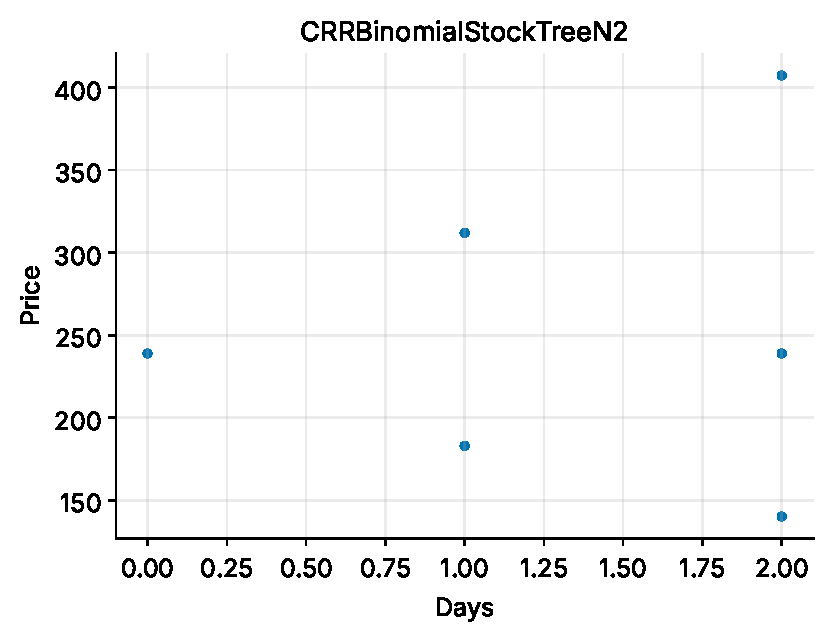
\includegraphics[width=0.48\textwidth]{crr_stock_tree_N2.pdf}\hfill
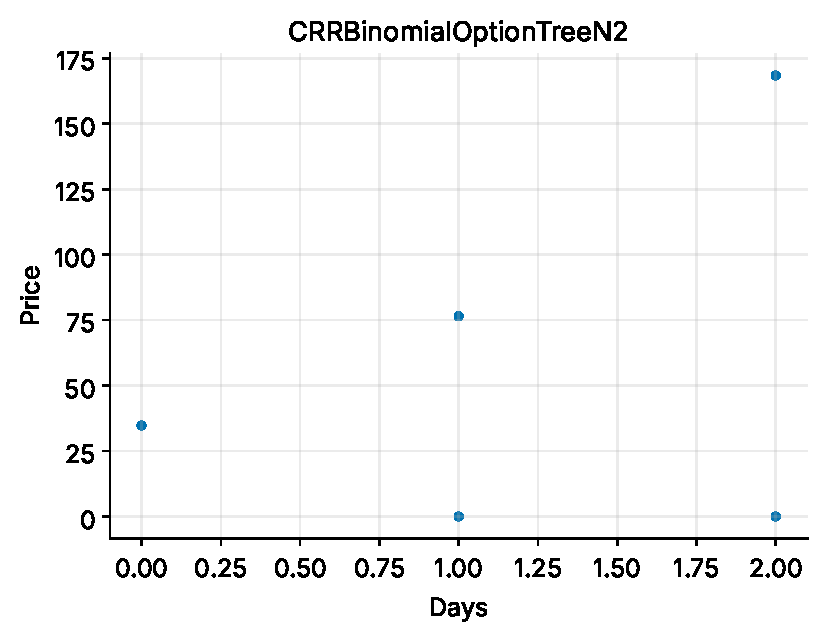
\includegraphics[width=0.48\textwidth]{crr_option_tree_N2.pdf}
\caption{CRR stock tree (left) and option tree (right), $N=2$.}
\end{figure}
\begin{figure}[h!]
\centering
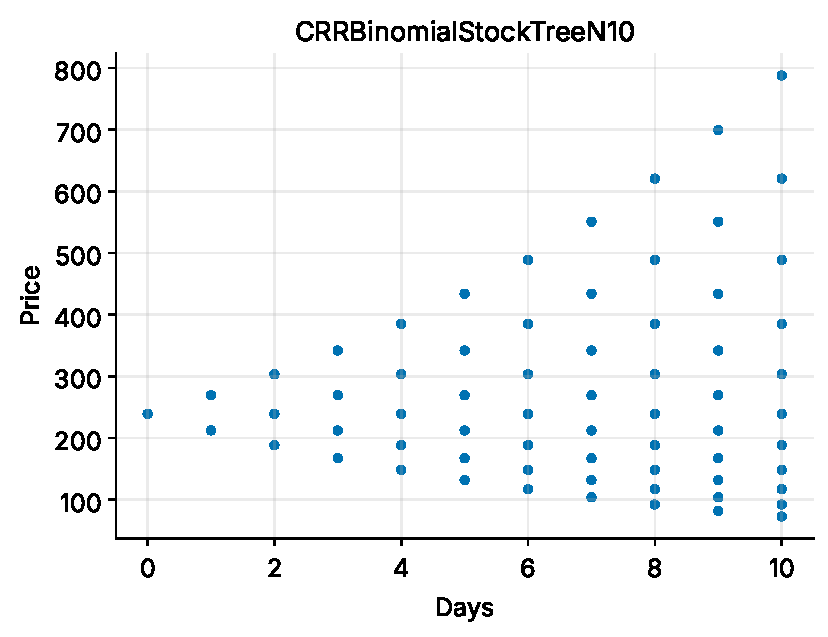
\includegraphics[width=0.48\textwidth]{crr_stock_tree_N10.pdf}\hfill
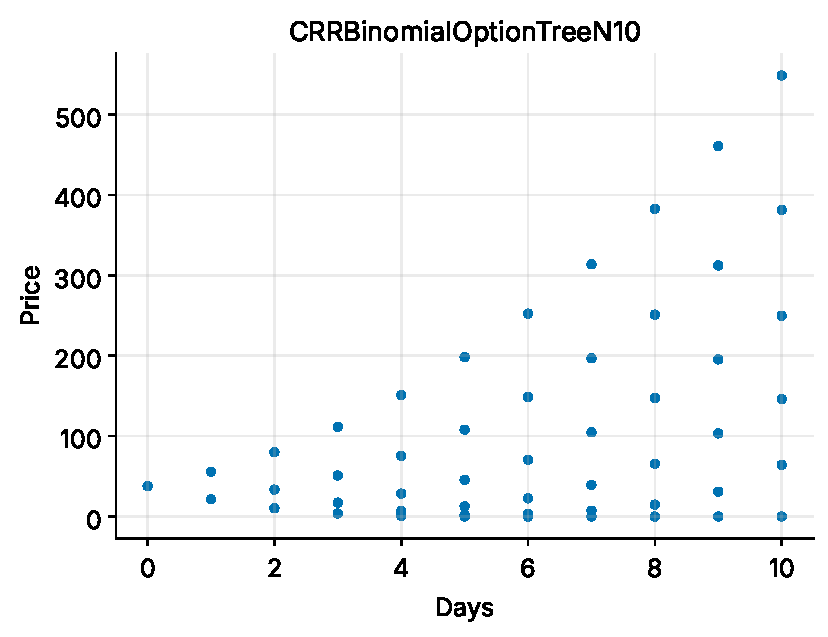
\includegraphics[width=0.48\textwidth]{crr_option_tree_N10.pdf}
\caption{CRR stock tree (left) and option tree (right), $N=10$.}
\end{figure}
\begin{figure}[h!]
\centering
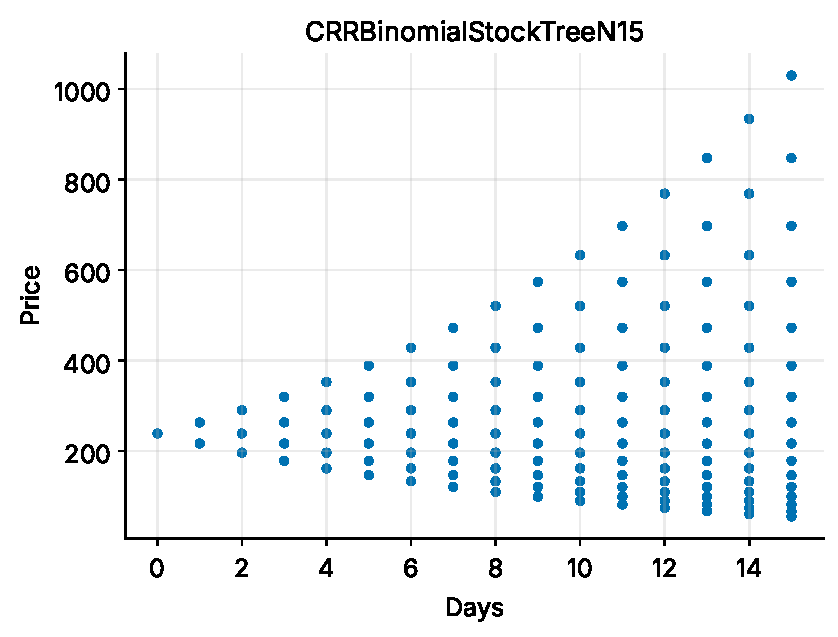
\includegraphics[width=0.48\textwidth]{crr_stock_tree_N15.pdf}\hfill
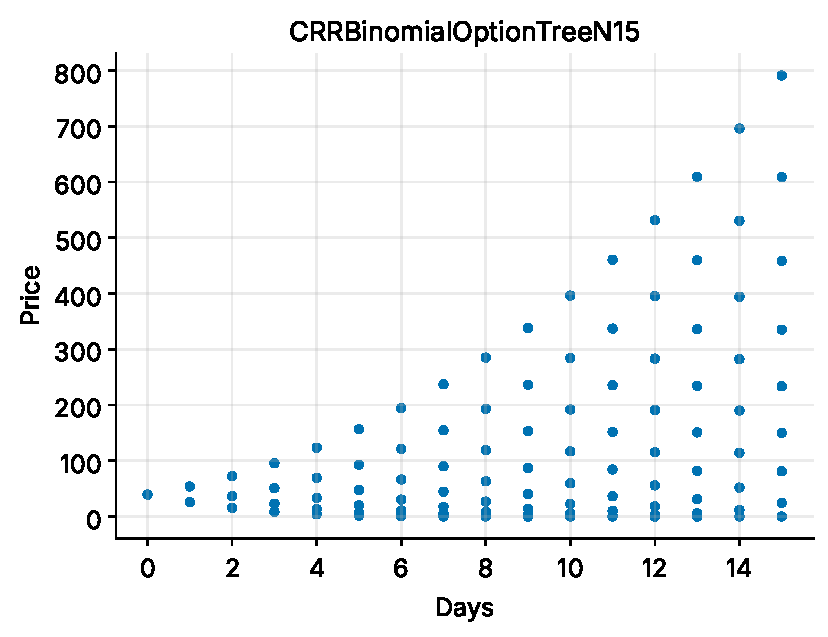
\includegraphics[width=0.48\textwidth]{crr_option_tree_N15.pdf}
\caption{CRR stock tree (left) and option tree (right), $N=15$.}
\end{figure}
\begin{figure}[h!]
\centering
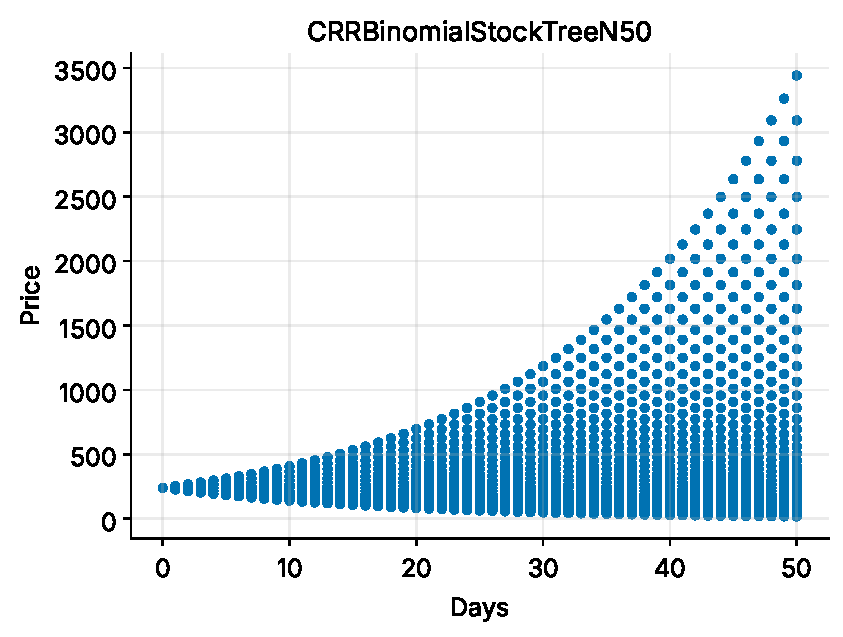
\includegraphics[width=0.48\textwidth]{crr_stock_tree_N50.pdf}\hfill
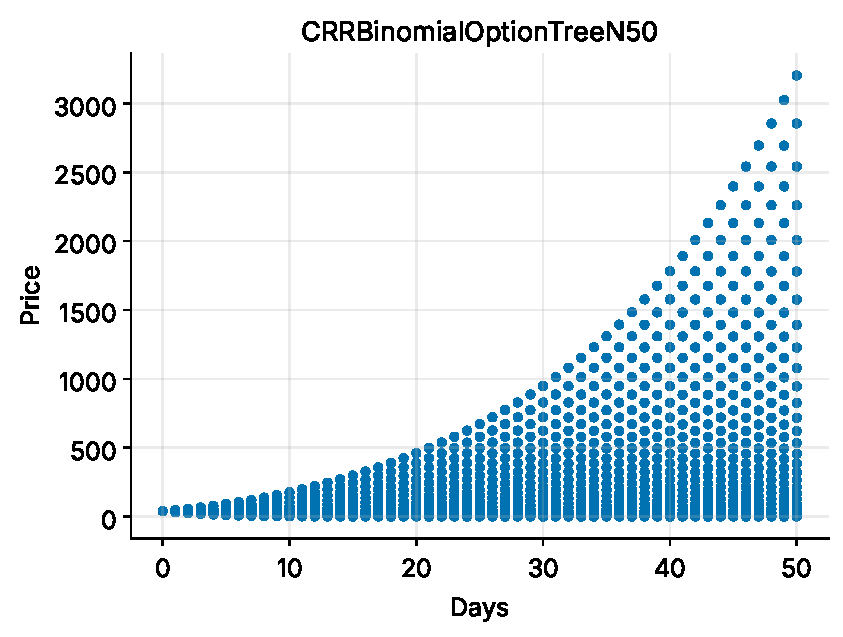
\includegraphics[width=0.48\textwidth]{crr_option_tree_N50.pdf}
\caption{CRR stock tree (left) and option tree (right), $N=50$.}
\end{figure}
\begin{figure}[h!]
\centering
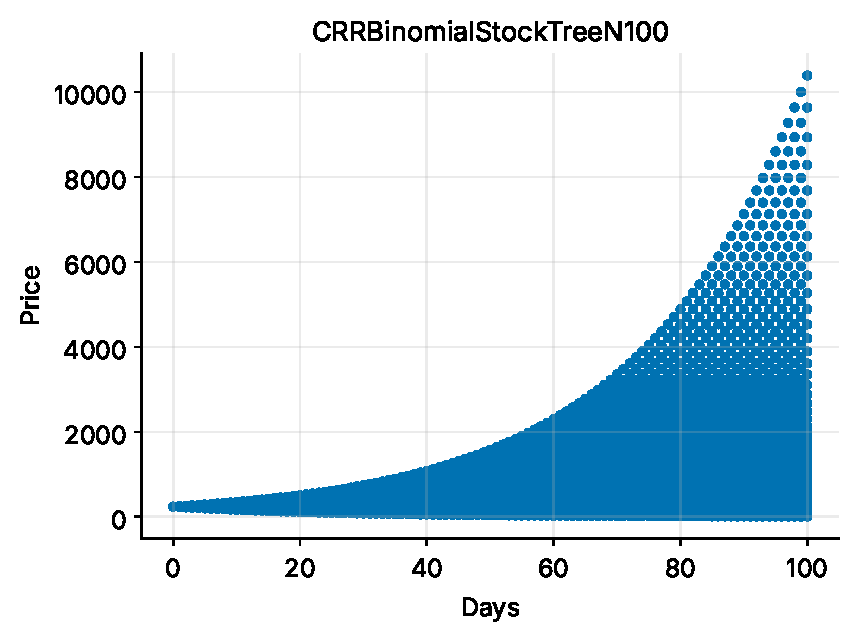
\includegraphics[width=0.48\textwidth]{crr_stock_tree_N100.pdf}\hfill
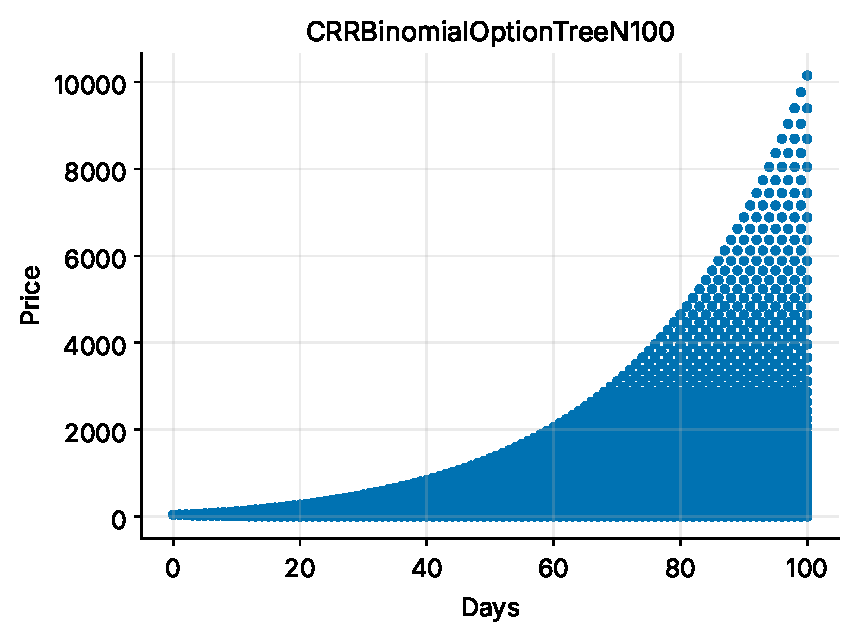
\includegraphics[width=0.48\textwidth]{crr_option_tree_N100.pdf}
\caption{CRR stock tree (left) and option tree (right), $N=100$.}
\end{figure}
\FloatBarrier

\clearpage
\section{Code}\label{app:code}
The listing shows the hand-written classes and functions exactly as used in the notebook, followed by the extensions that are built on top of them. The full notebook (with the experiments) is \texttt{notebooks/option\_pricing.ipynb}.
\subsection*{Hand-written classes and functions}
\begin{multicols}{2}
\lstinputlisting{code/handwritten.py}
\end{multicols}
\subsection*{Extensions}
\begin{multicols}{2}
\lstinputlisting{code/extensions.py}
\end{multicols}

\nocite{*}
\bibliographystyle{plainnat}
\bibliography{references}

\end{document}
